\mychapter{기초개념 확인하기}{그래프를 본격적으로 배우기 전에 좌표평면, 함수의 그래프, 부등식의 영역에 대한 기초개념을 간단하고 빠르게 배워봅시다.}

\section{$\xy xy$는 좌표평면 전체를 나타낸다}

\begin{figure}[h]\centering \subfloat[][]{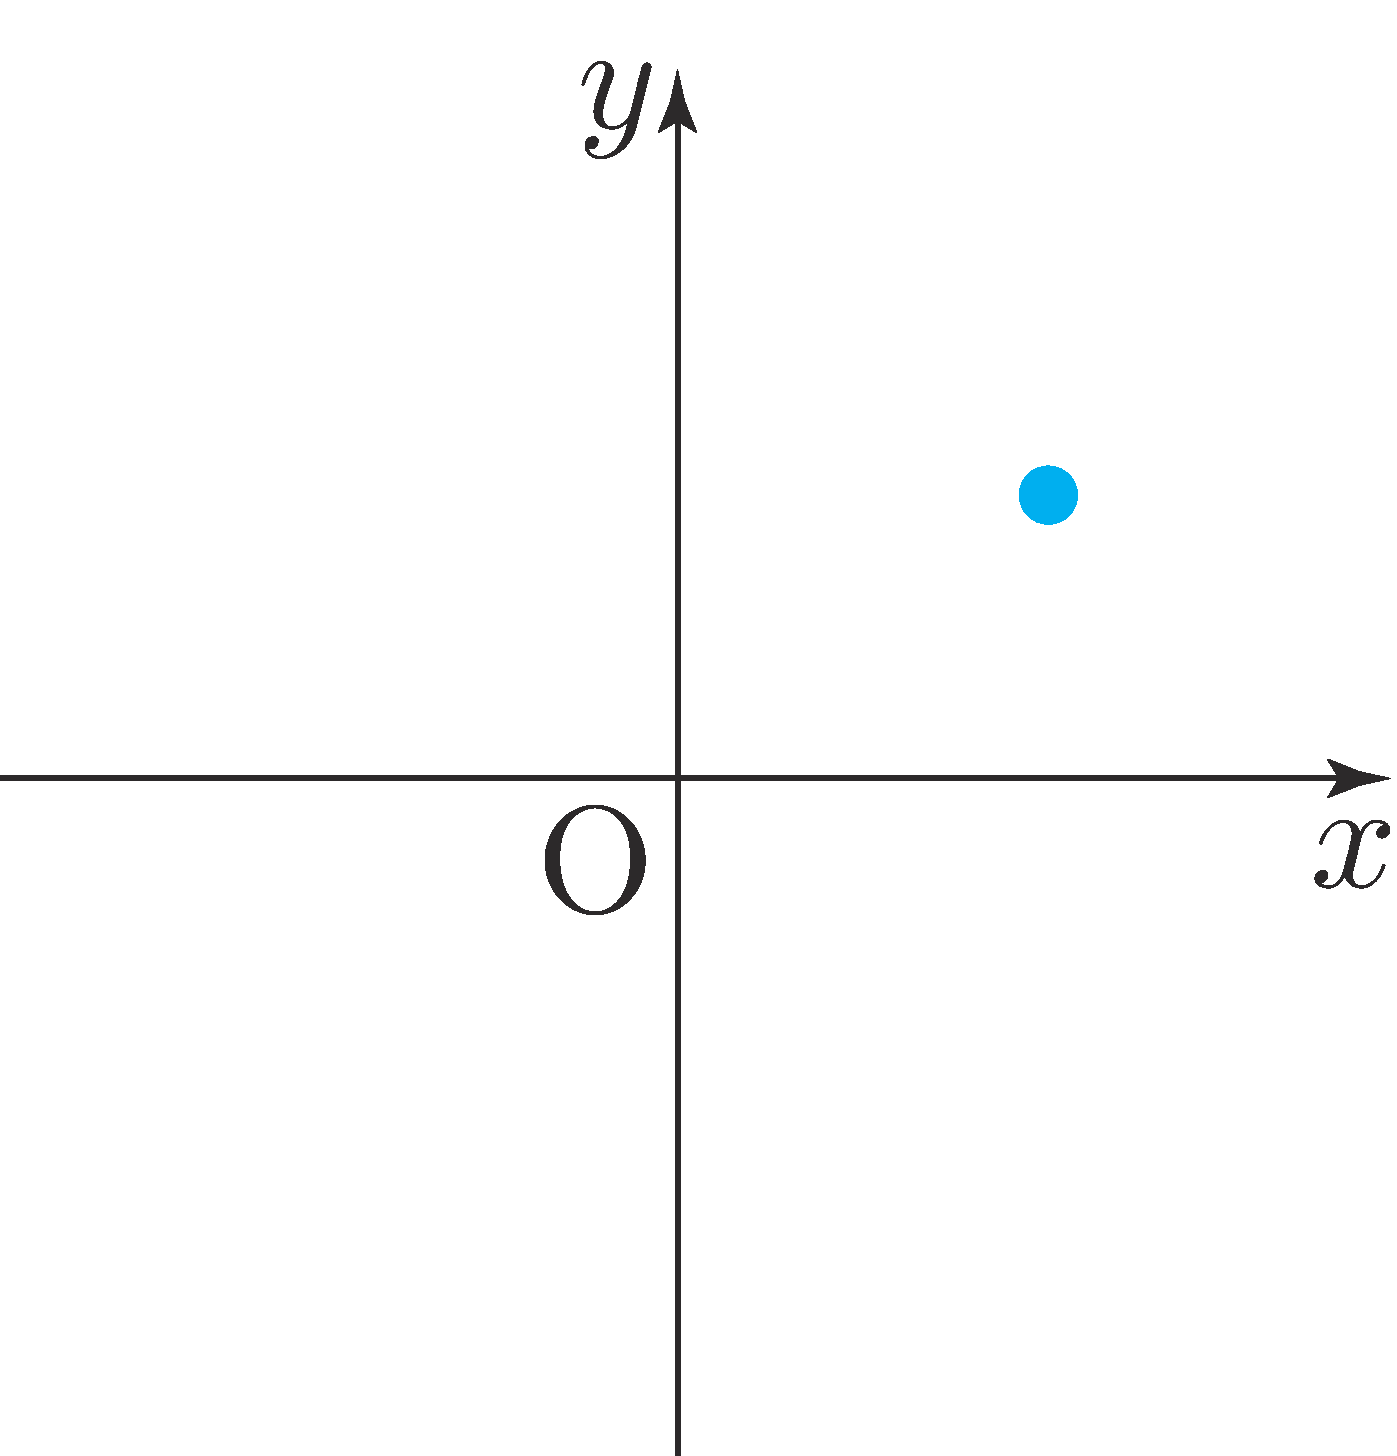
\includegraphics[scale=\pgfkeysvalueof{picsize}]{DBs/pic/zery_01_1.pdf}}\
\qquad\qquad
\centering \subfloat[][]{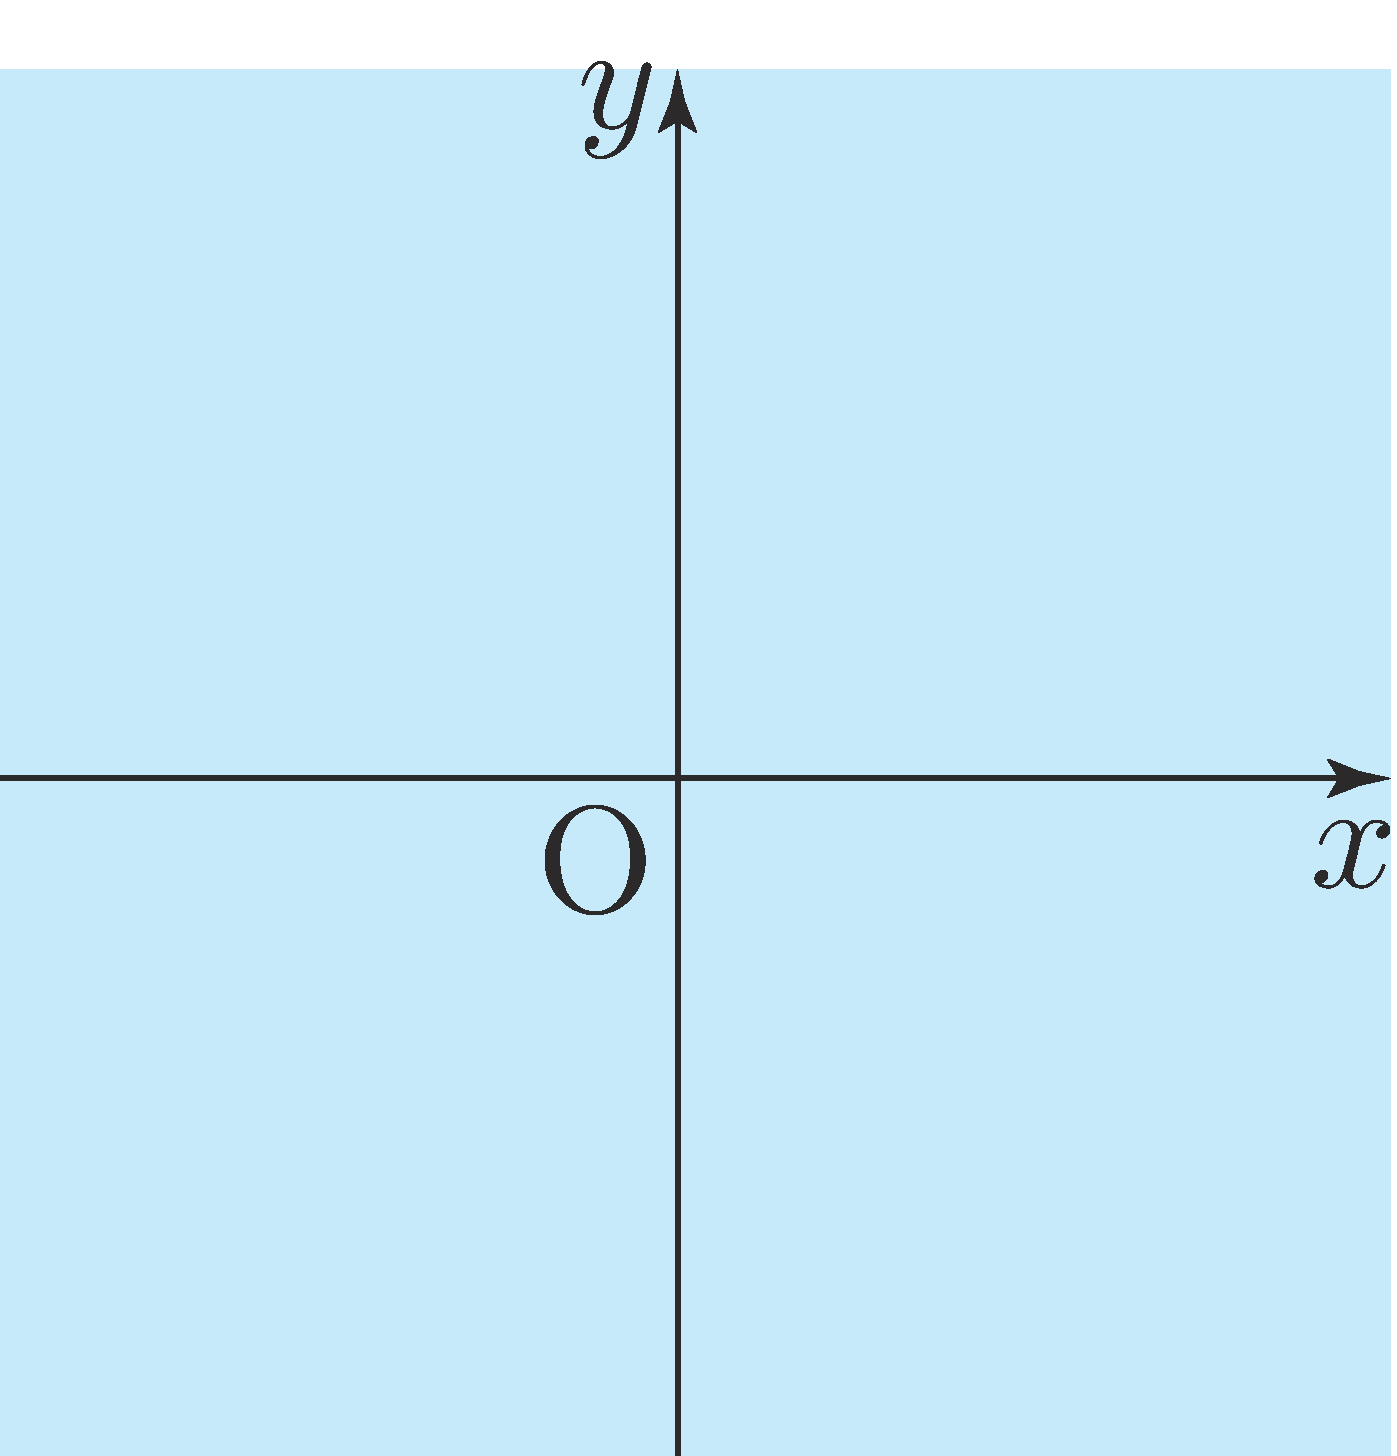
\includegraphics[scale=\pgfkeysvalueof{picsize}]{DBs/pic/zery_01_2.pdf}}\
\end{figure}


일반적으로 좌표평면 위의 점 $\xy xy$라 하면, $x$와 $y$에 아무런 제약이 없으므로 $x$는 임의의 실수, $y$는 임의의 실수입니다. 따라서 $\xy xy$가 나타내는 영역을 색칠하면 (b)와 같이 좌표평면 전체를 칠하게 됩니다.

\section{$x=k$와 $y=k$가 나타내는 도형}

\begin{figure}[h]
	\centering \subfloat[][]{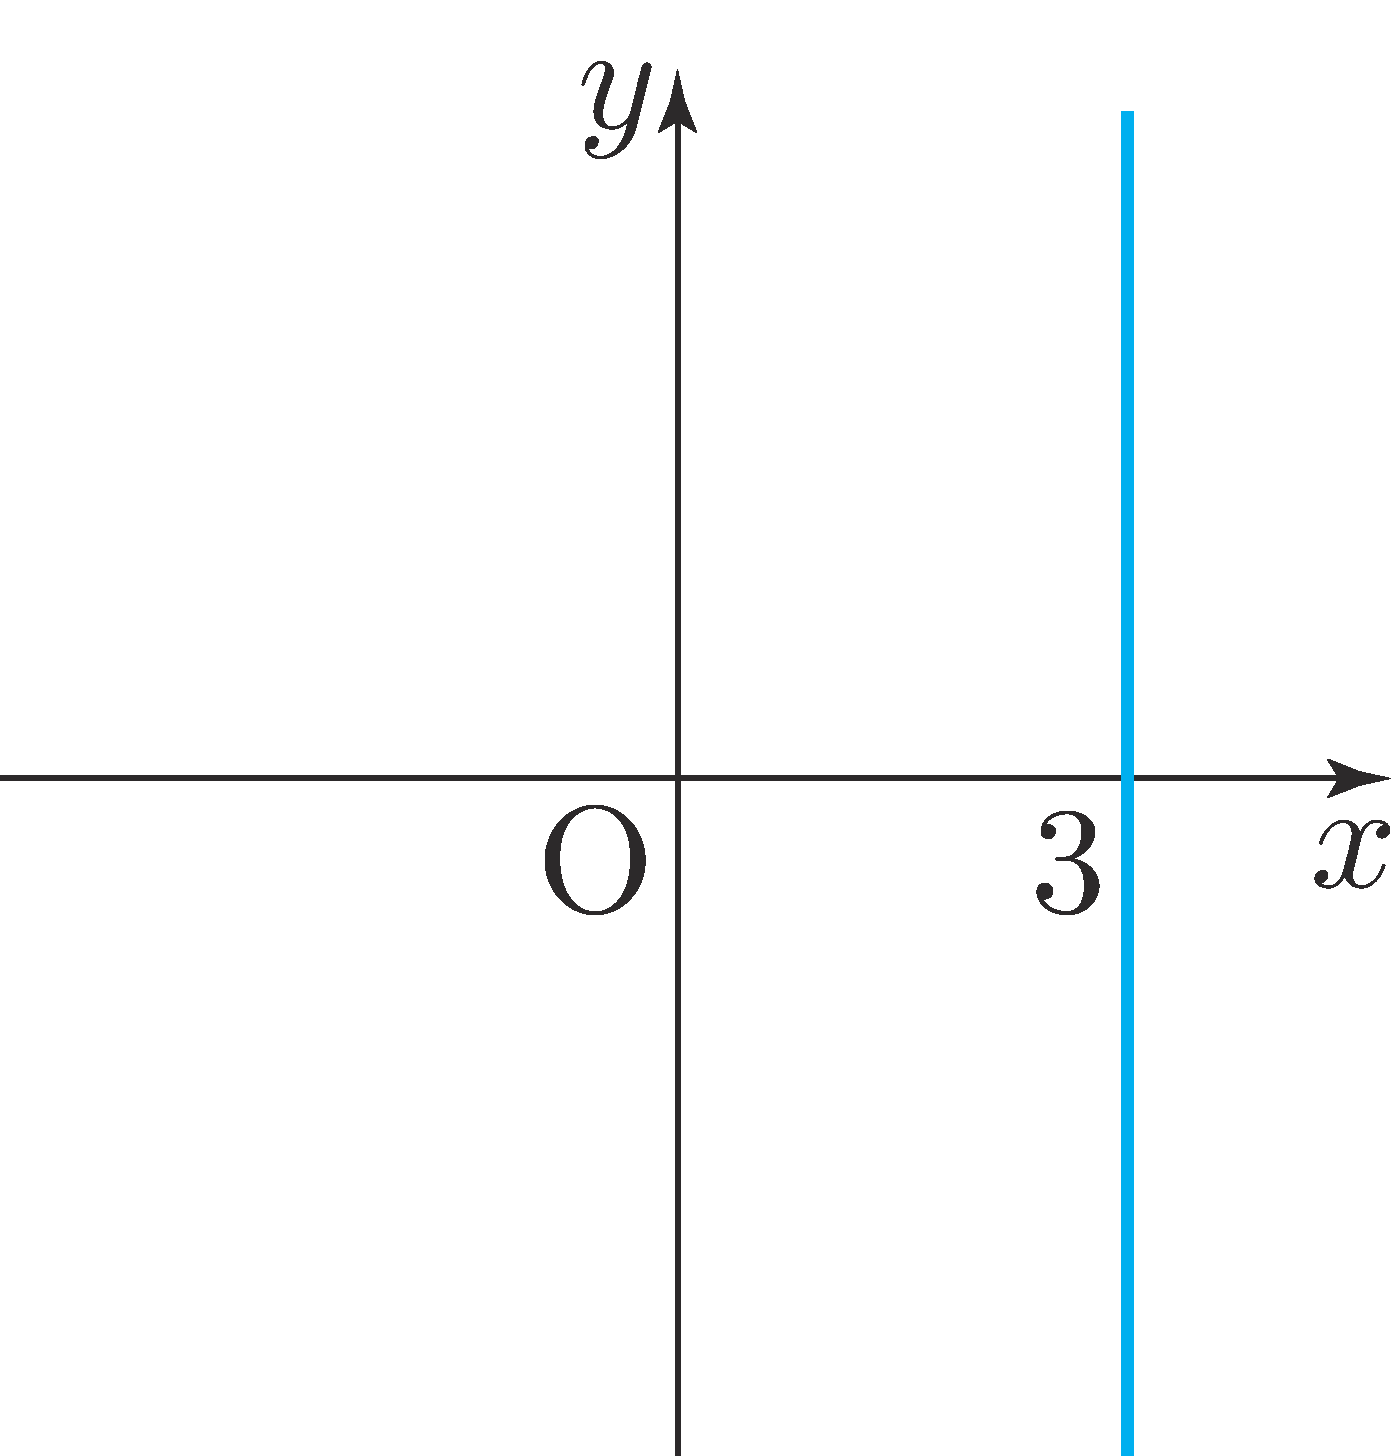
\includegraphics[scale=\pgfkeysvalueof{picsize}]{DBs/pic/zery_02_1.pdf}}\
	\qquad\qquad
	\centering \subfloat[][]{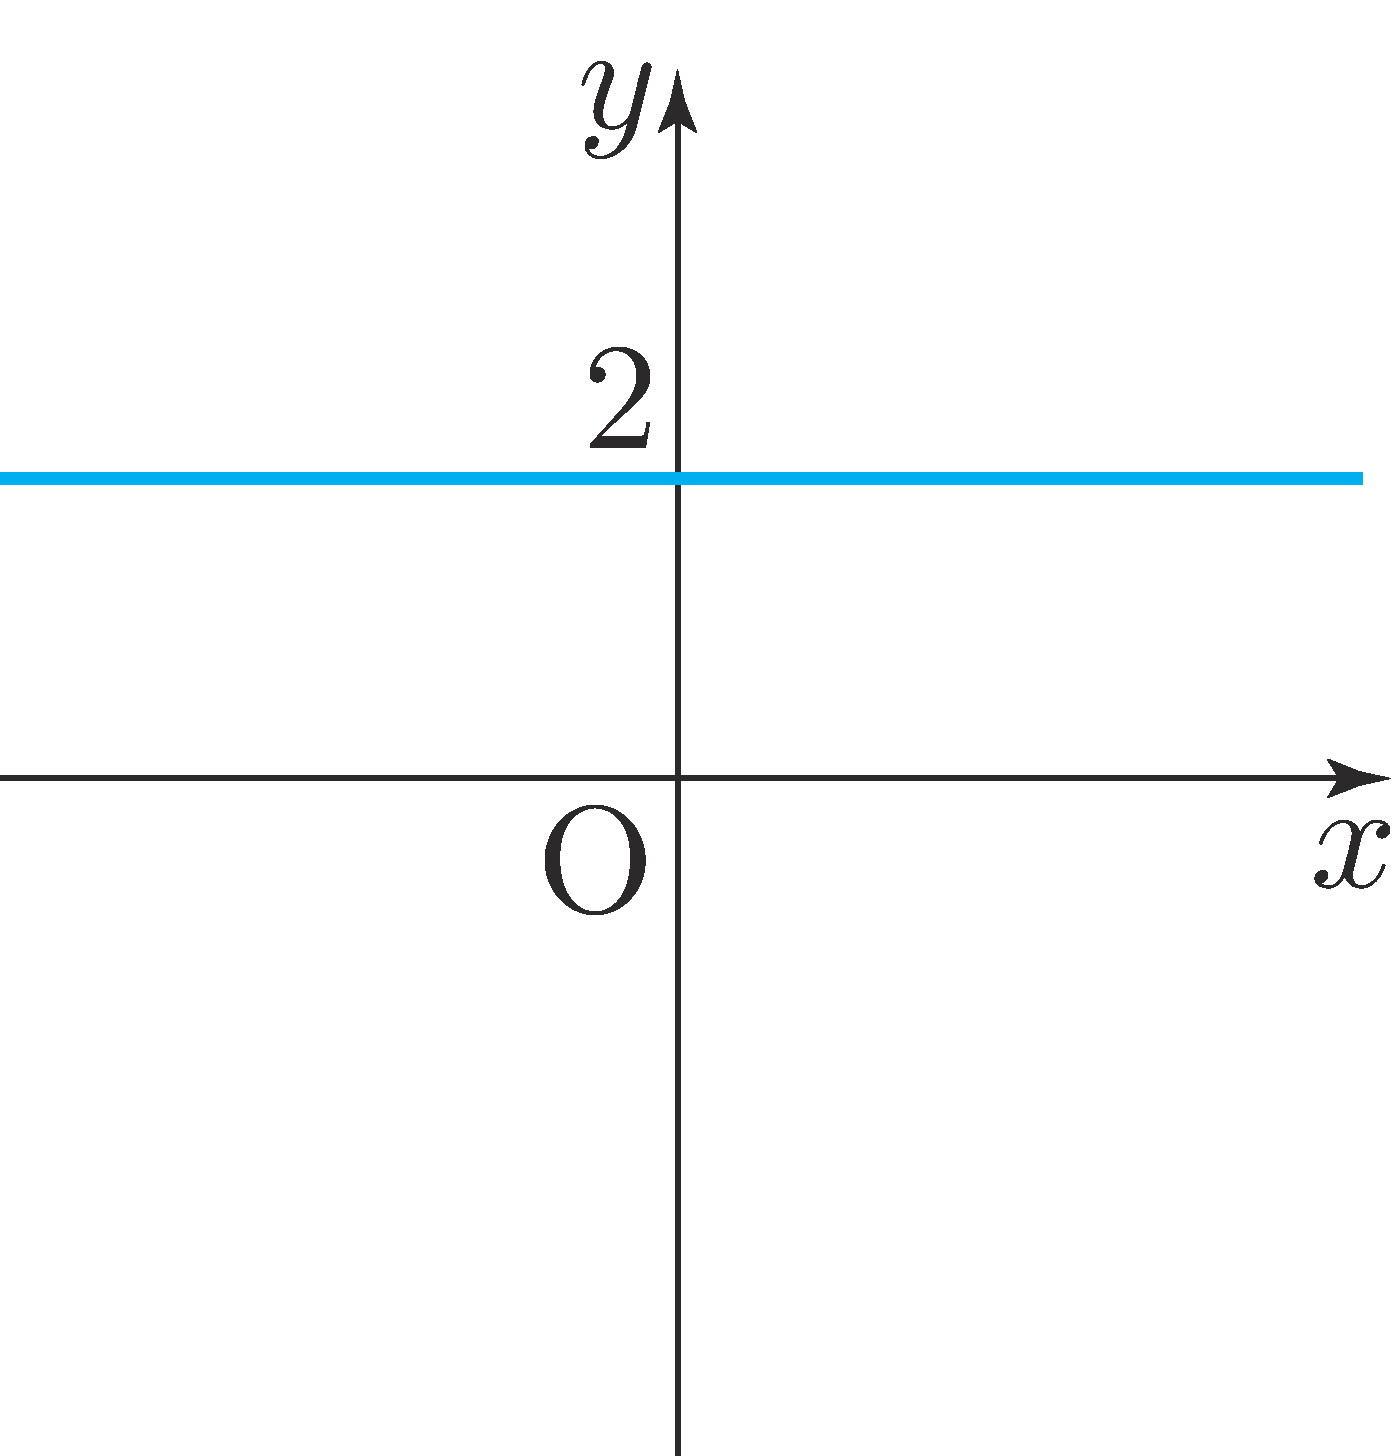
\includegraphics[scale=\pgfkeysvalueof{picsize}]{DBs/pic/zery_02_2.pdf}}\
	\end{figure}

	
	$x=3$이라는 방정식은 $\xy{3}{y}$라 할 수 있고, $x$는 상수 $3$으로 고정, $y$는 임의의 실수입니다. 이러한 점들은 (a)와 같이 좌표평면에서 $x$축에 수직이고 $\xy 30$을 지나는 직선을 나타냅니다. $y=2$라는 직선도 마찬가지 방법으로 (b)와 같이 $y$축에 수직이고 $\xy 02$를 지나는 직선을 나타내게 됩니다.
\clearpage
\section{$y=f\left( x \right) $가 나타내는 도형}

\begin{figure}[h]
	\centering \subfloat[][]{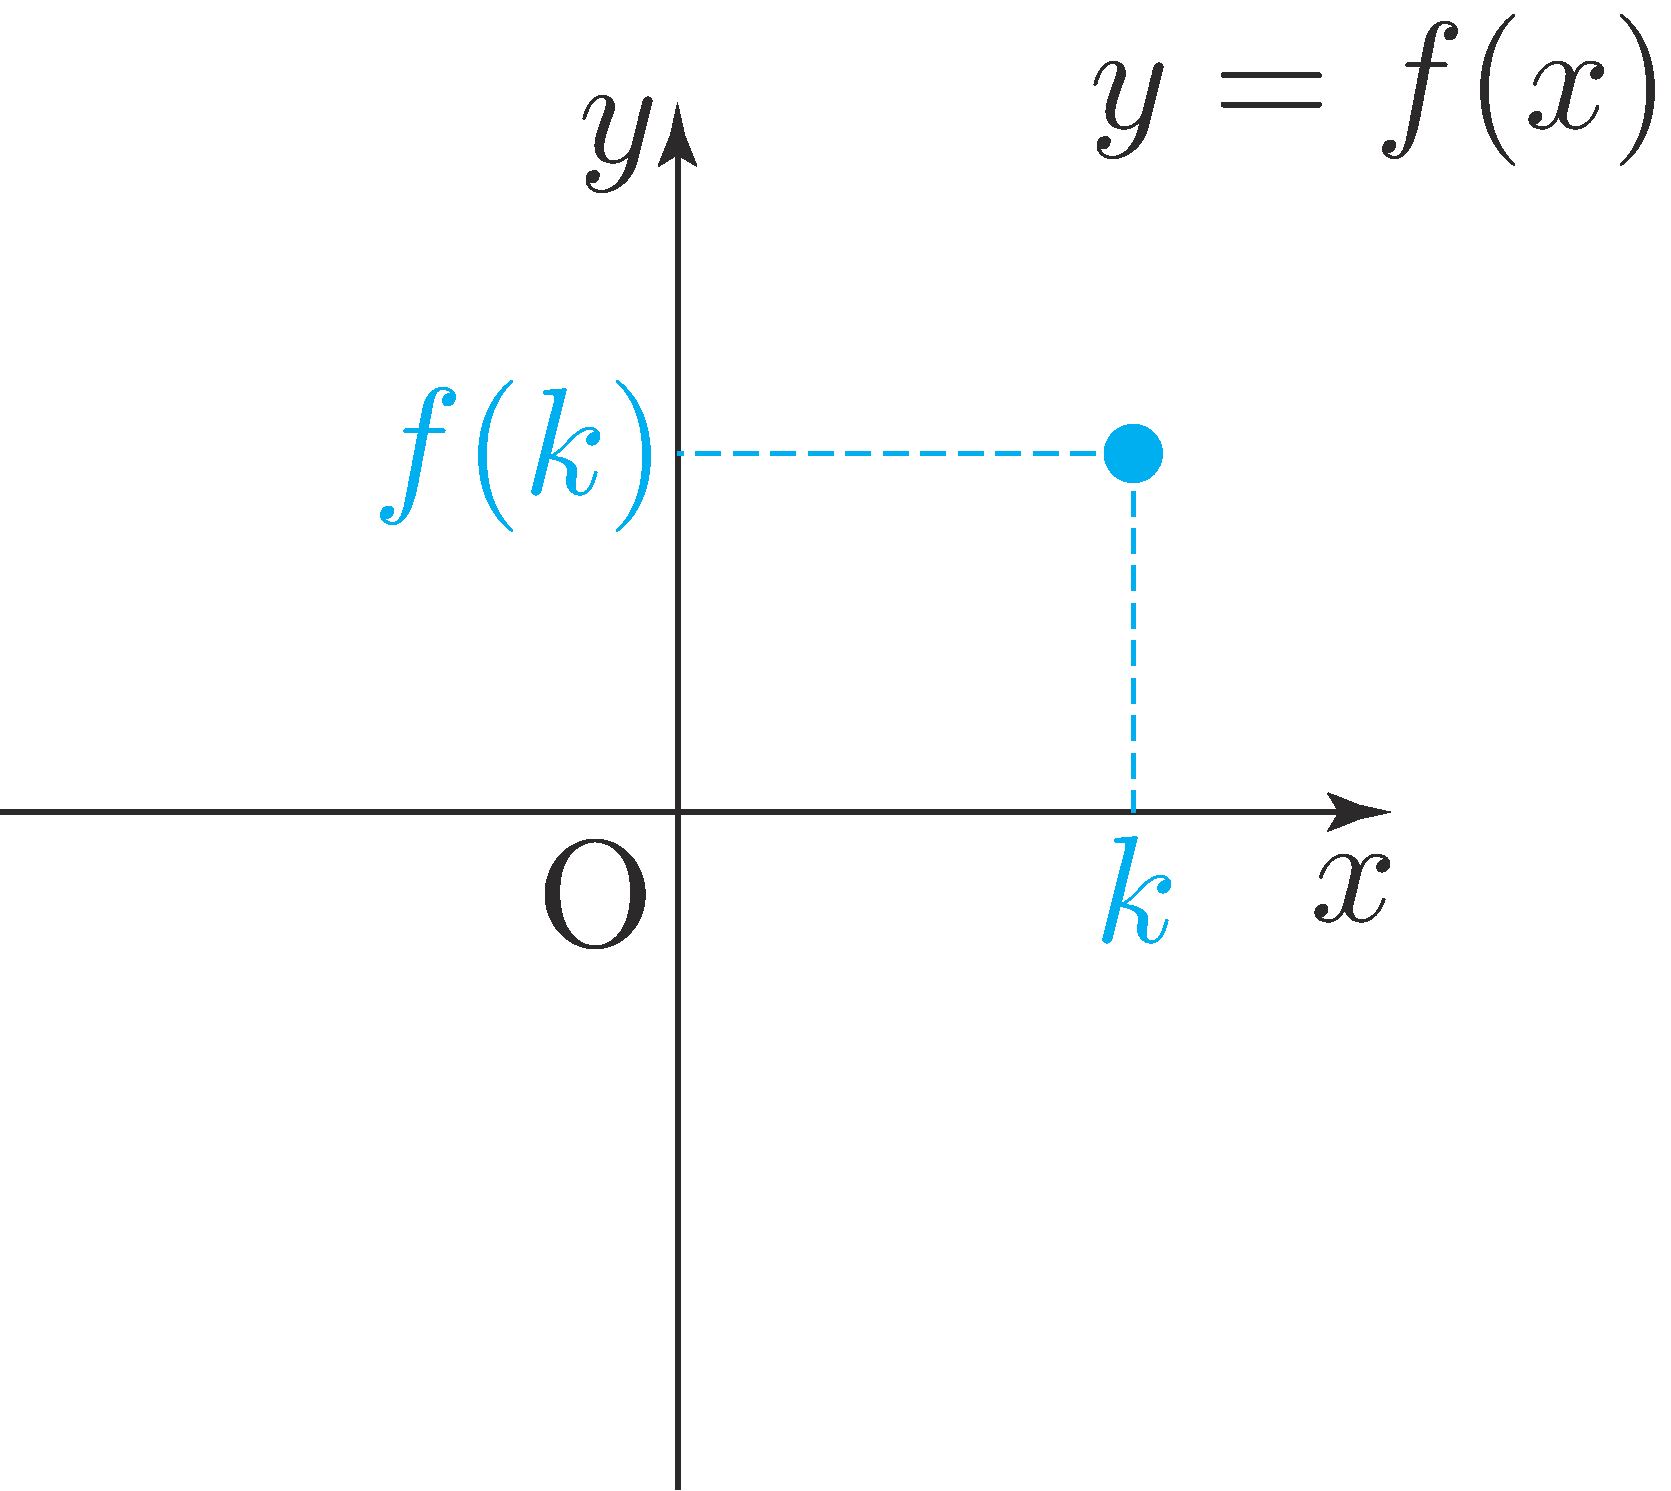
\includegraphics[scale=\pgfkeysvalueof{picsize}]{DBs/pic/zery_03.pdf}}\
	\qquad\qquad
	\centering \subfloat[][]{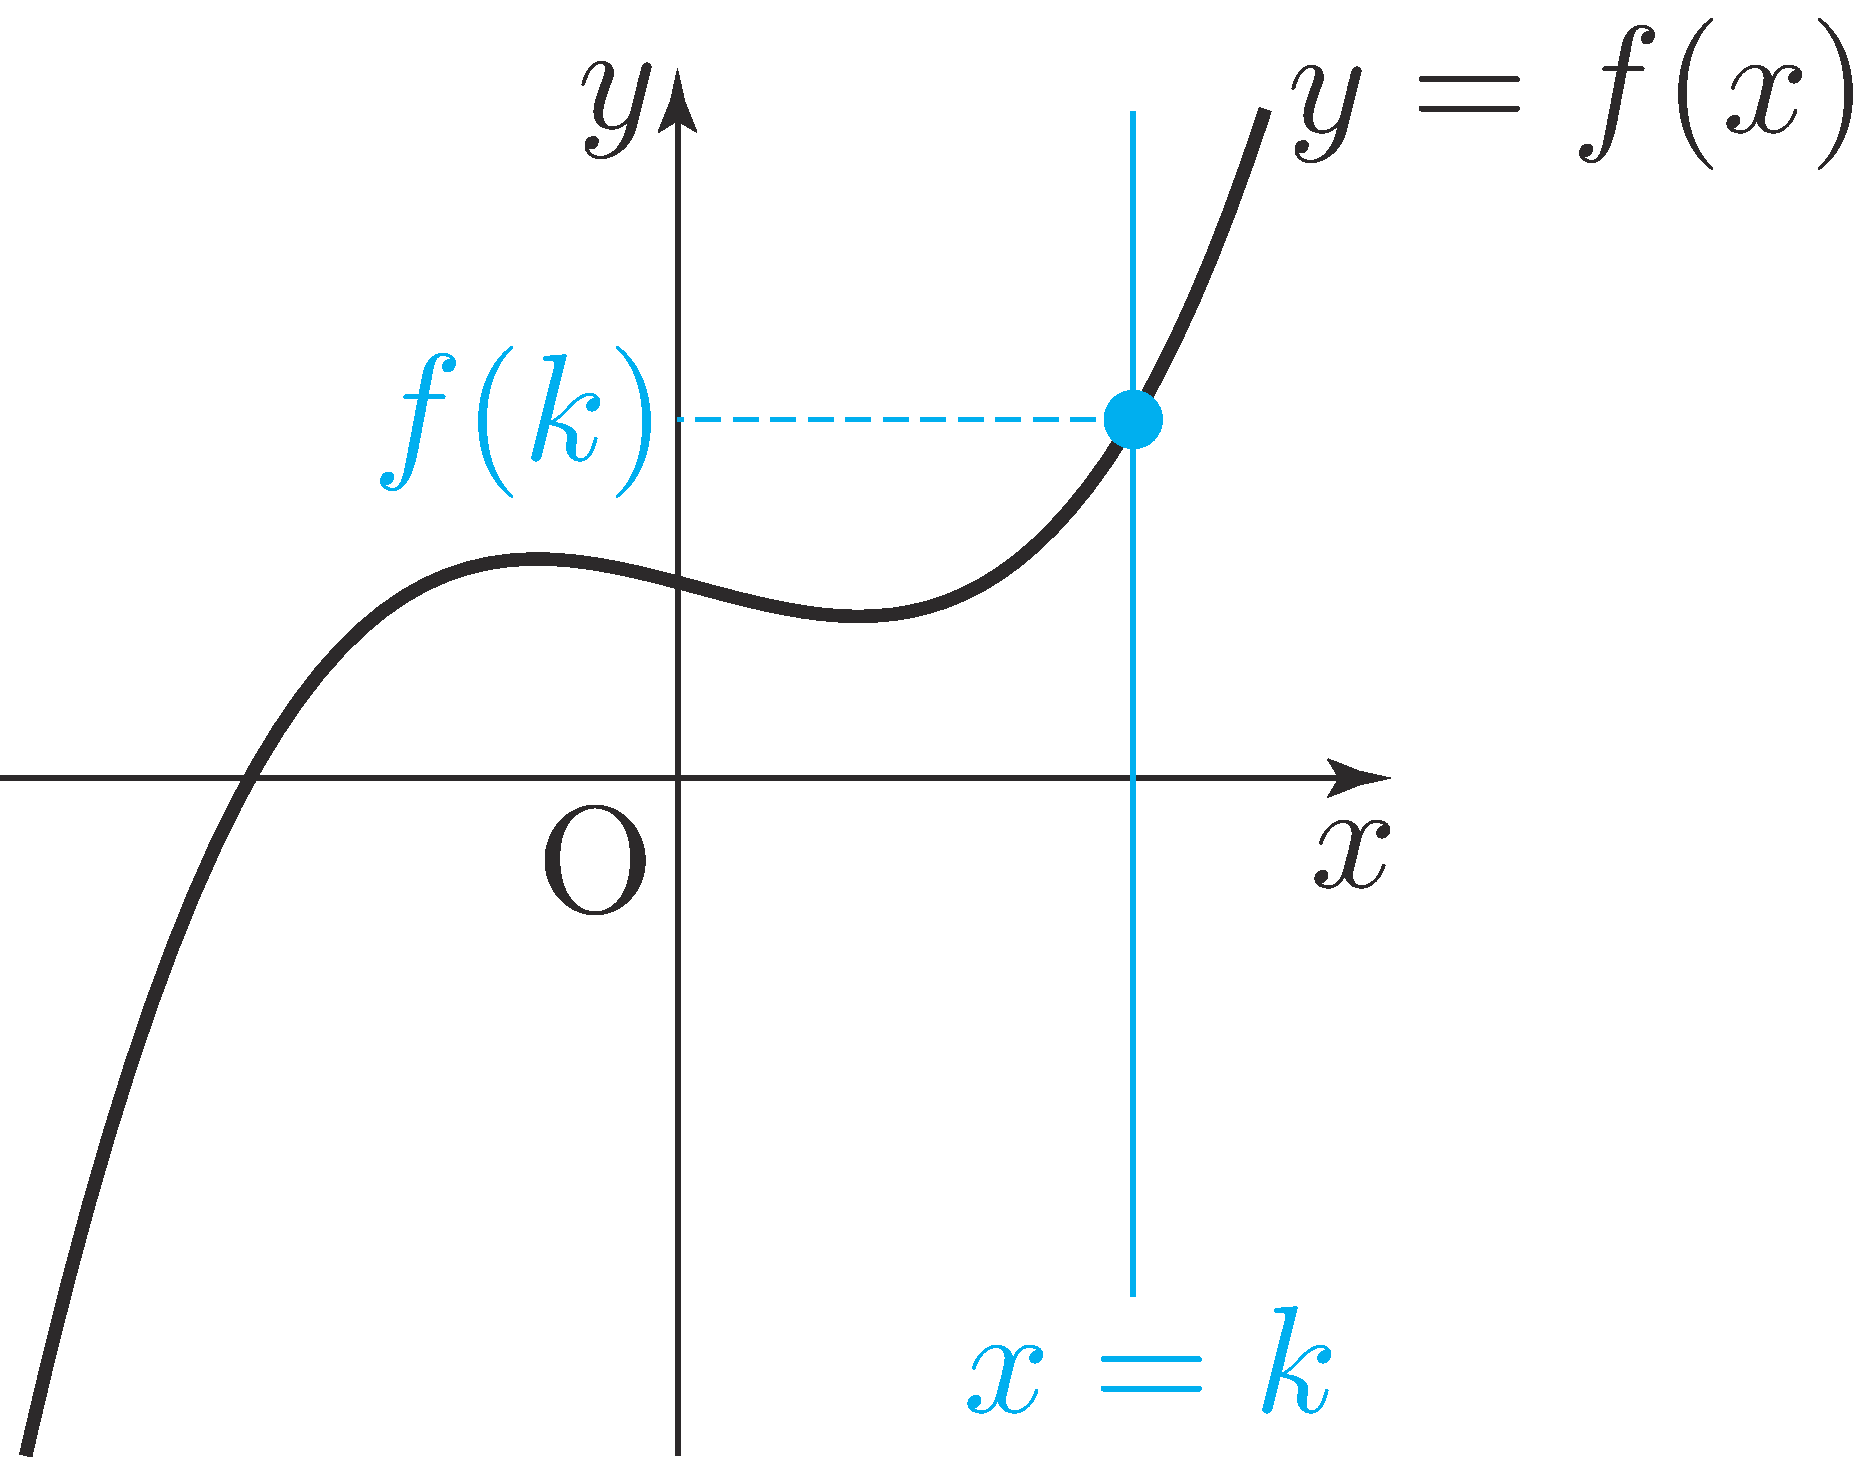
\includegraphics[scale=\pgfkeysvalueof{picsize}]{DBs/pic/zery_04.pdf}}\
	\end{figure}

	
	앞에서와 같은 방법으로 $y=f\left( x \right) $라는 식을 해석하면, $x$에는 제약이 없고\mn{여기까지만 보았을 때는 제약이 없어 보입니다.}{}, $y$에는 $f\left( x \right) $라는 제약이 생깁니다. 그러면 $x$좌표가 $k$일 때 $y$좌표가 $f\left( k \right) $인 점을 찍으면 됩니다.  즉 $x$좌표는 $x$를 취하고, $y$좌표는 (해당하는 $x$에 대하여 오직 하나의 값인) $f\left( x \right) $를 취하여 점을 찍기 때문에, 방정식의 이름이 $y = f\left( x \right) $인 것입니다.

그런데 함수의 제약조건 (2)에 의해 $k$ 하나에 대응되는 $f\left( k \right) $는 유일하므로 $x=k$와 $y=f\left( x \right) $가 만나는 점은 오직 $\xy{k}{f\left( k \right) }$로 유일합니다. 주어진 그래프가 함수의 그래프인지 따질 때 $x$축에 수직인 직선을 그어 교점의 개수가 $2$ 이상인 경우를 거르는 것은 이 때문입니다.
\begin{center} 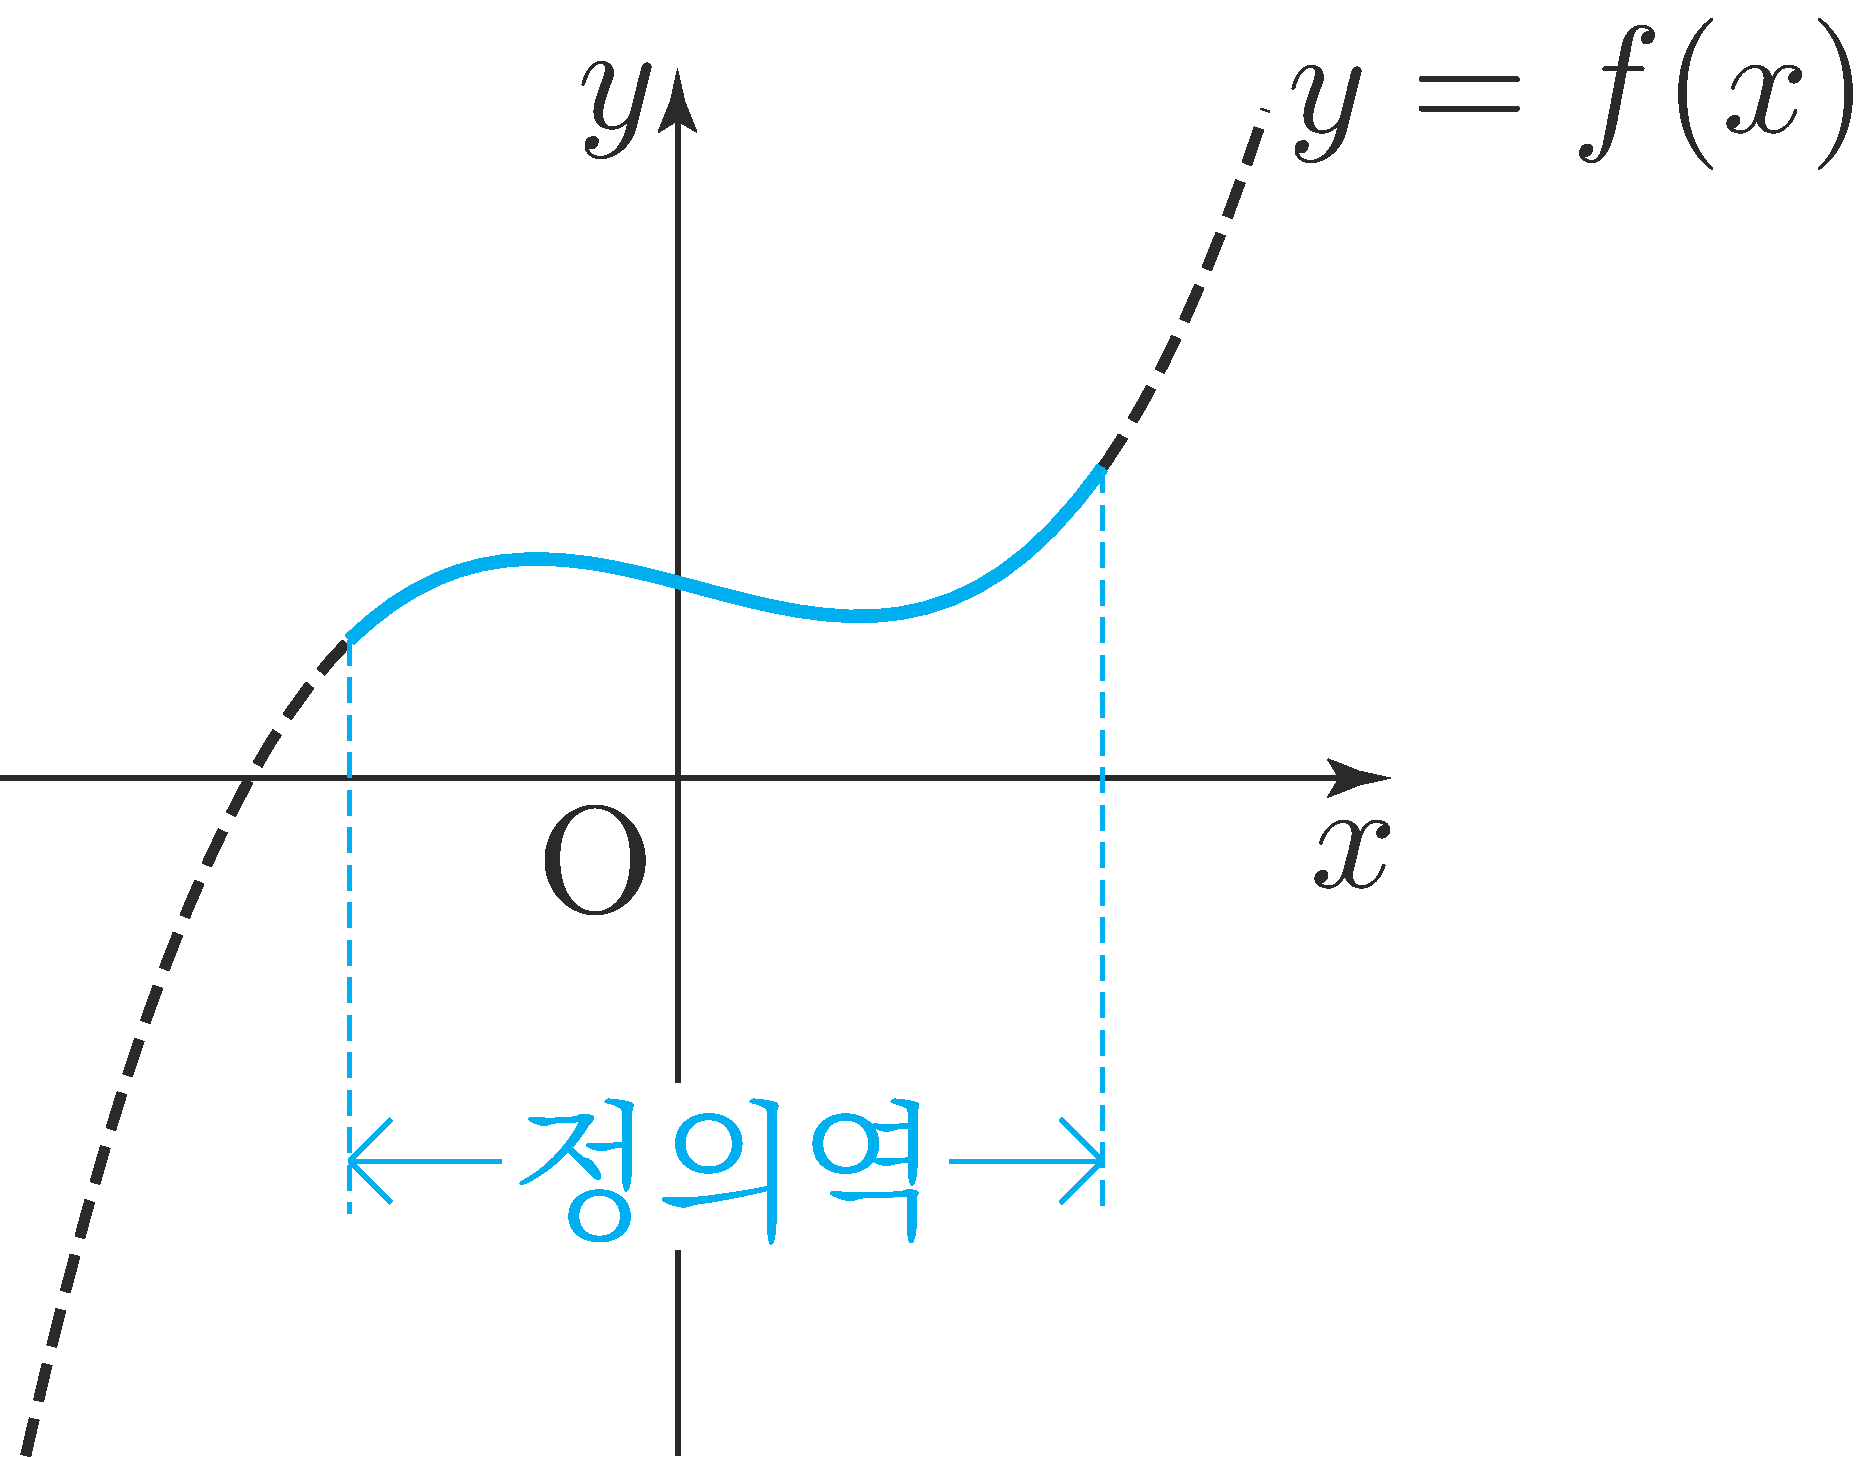
\includegraphics[scale=\pgfkeysvalueof{picsize}]{DBs/pic/zery_05.pdf}\
	\end{center}한편, 앞서 $x$좌표에는 제약이 없어 보였지만, 잘 생각해보면 $f\left( k \right) $는 $k$가 $f\left( x \right) $의 정의역의 원소일 때에만 정의되는 값입니다. 따라서 `$k$가 $f$의 정의역의 원소'라는 제약이 간접적으로 주어진 셈이 됩니다. 따라서 정의역은 좌표평면에서 $y=f\left( x \right) $가 그려지는 가로 범위를 결정합니다.
\clearpage
\section{기본적인 부등식이 나타내는 도형}
이 내용(부등식의 영역)은 교육과정에서 빠졌지만, 부등식과 좌표평면을 이해하고 미적분과 접목하는 데에 큰 도움이 되므로 소개합니다.\mn{평가원이 부등식의 영역을 직접 출제할 수는 없지만, 우리가 부등식의 영역을 이용하여 미적분을 해석하는 것을 막을 수는 없으니까요. 게다가 그다지 어려운 내용도 아닙니다.}{}
\begin{figure}[h]
	\centering \subfloat[][]{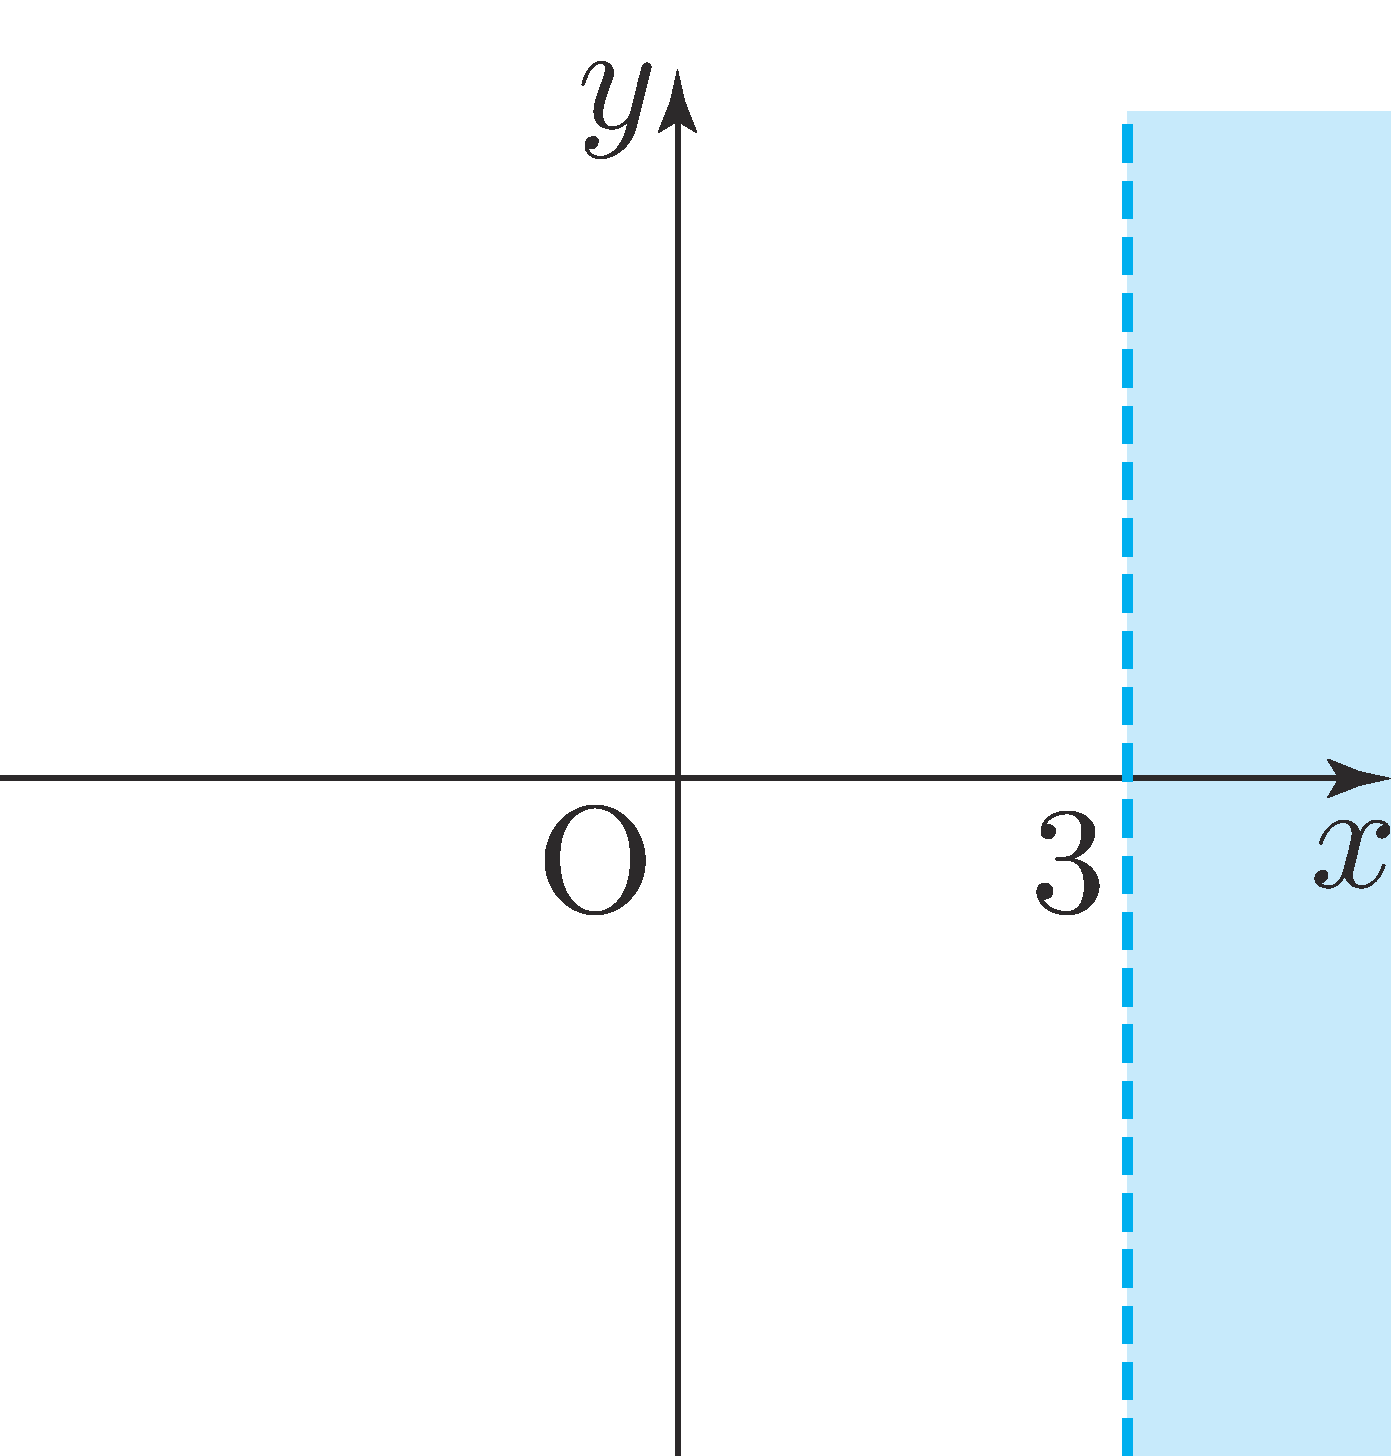
\includegraphics[scale=\pgfkeysvalueof{picsize}]{DBs/pic/zery_06_1.pdf}}\
	\qquad\qquad
	\centering \subfloat[][]{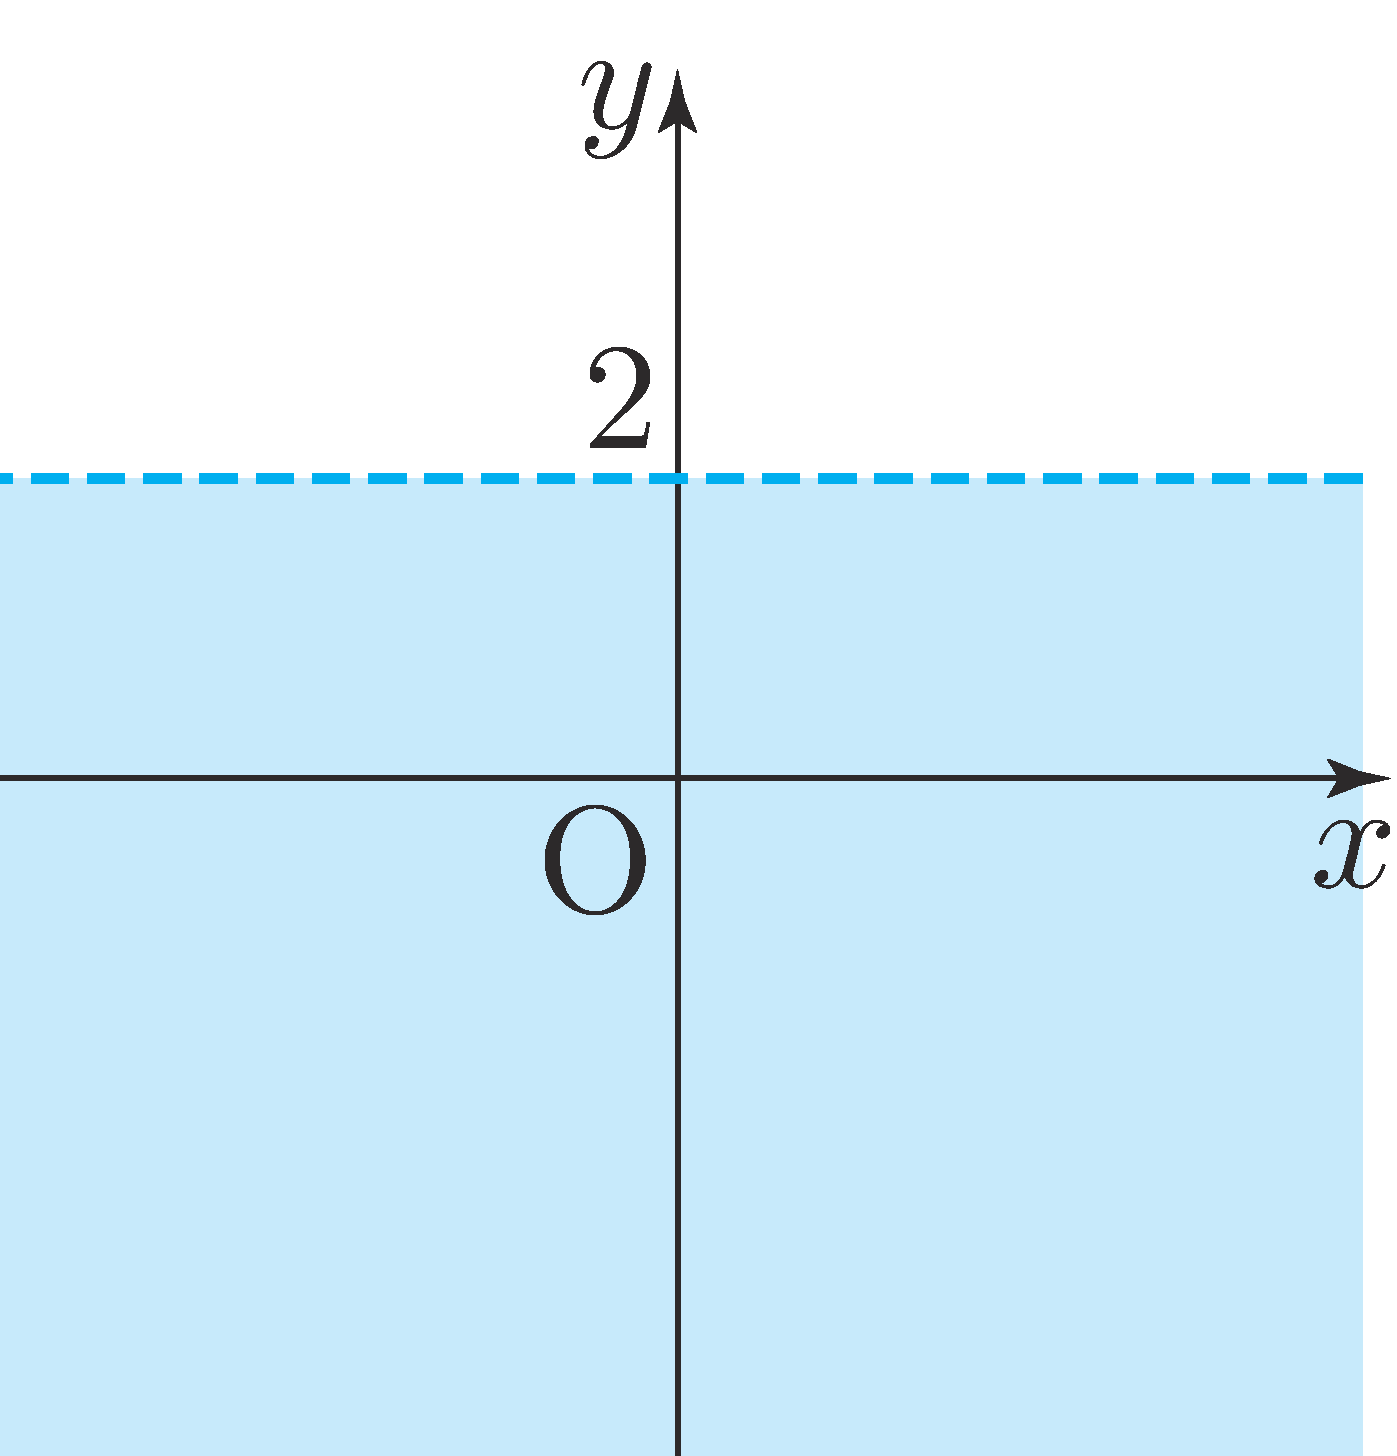
\includegraphics[scale=\pgfkeysvalueof{picsize}]{DBs/pic/zery_06_2.pdf}}\
	\end{figure}
좌표평면에서 $x>3$이라는 부등식은 $x$좌표가 $3$보다 큰 실수이고 $y$좌표는 임의의 실수인 점 $\xy{x}{y}$를 나타냅니다. 이러한 점들은 (a)와 같이 좌표평면에서 색칠된 영역을 나타냅니다. 직선 $x=3$은 이 영역의 경계가 됩니다. $y<2$라는 부등식도 마찬가지 방법으로 (b)와 같이 좌표평면에서 색칠된 영역을 나타내며, 직선 $y=2$는 이 영역의 경계가 됩니다.

\section{$y>f\left( x \right) $와 $y<f\left( x \right) $가 나타내는 도형}
\begin{center} 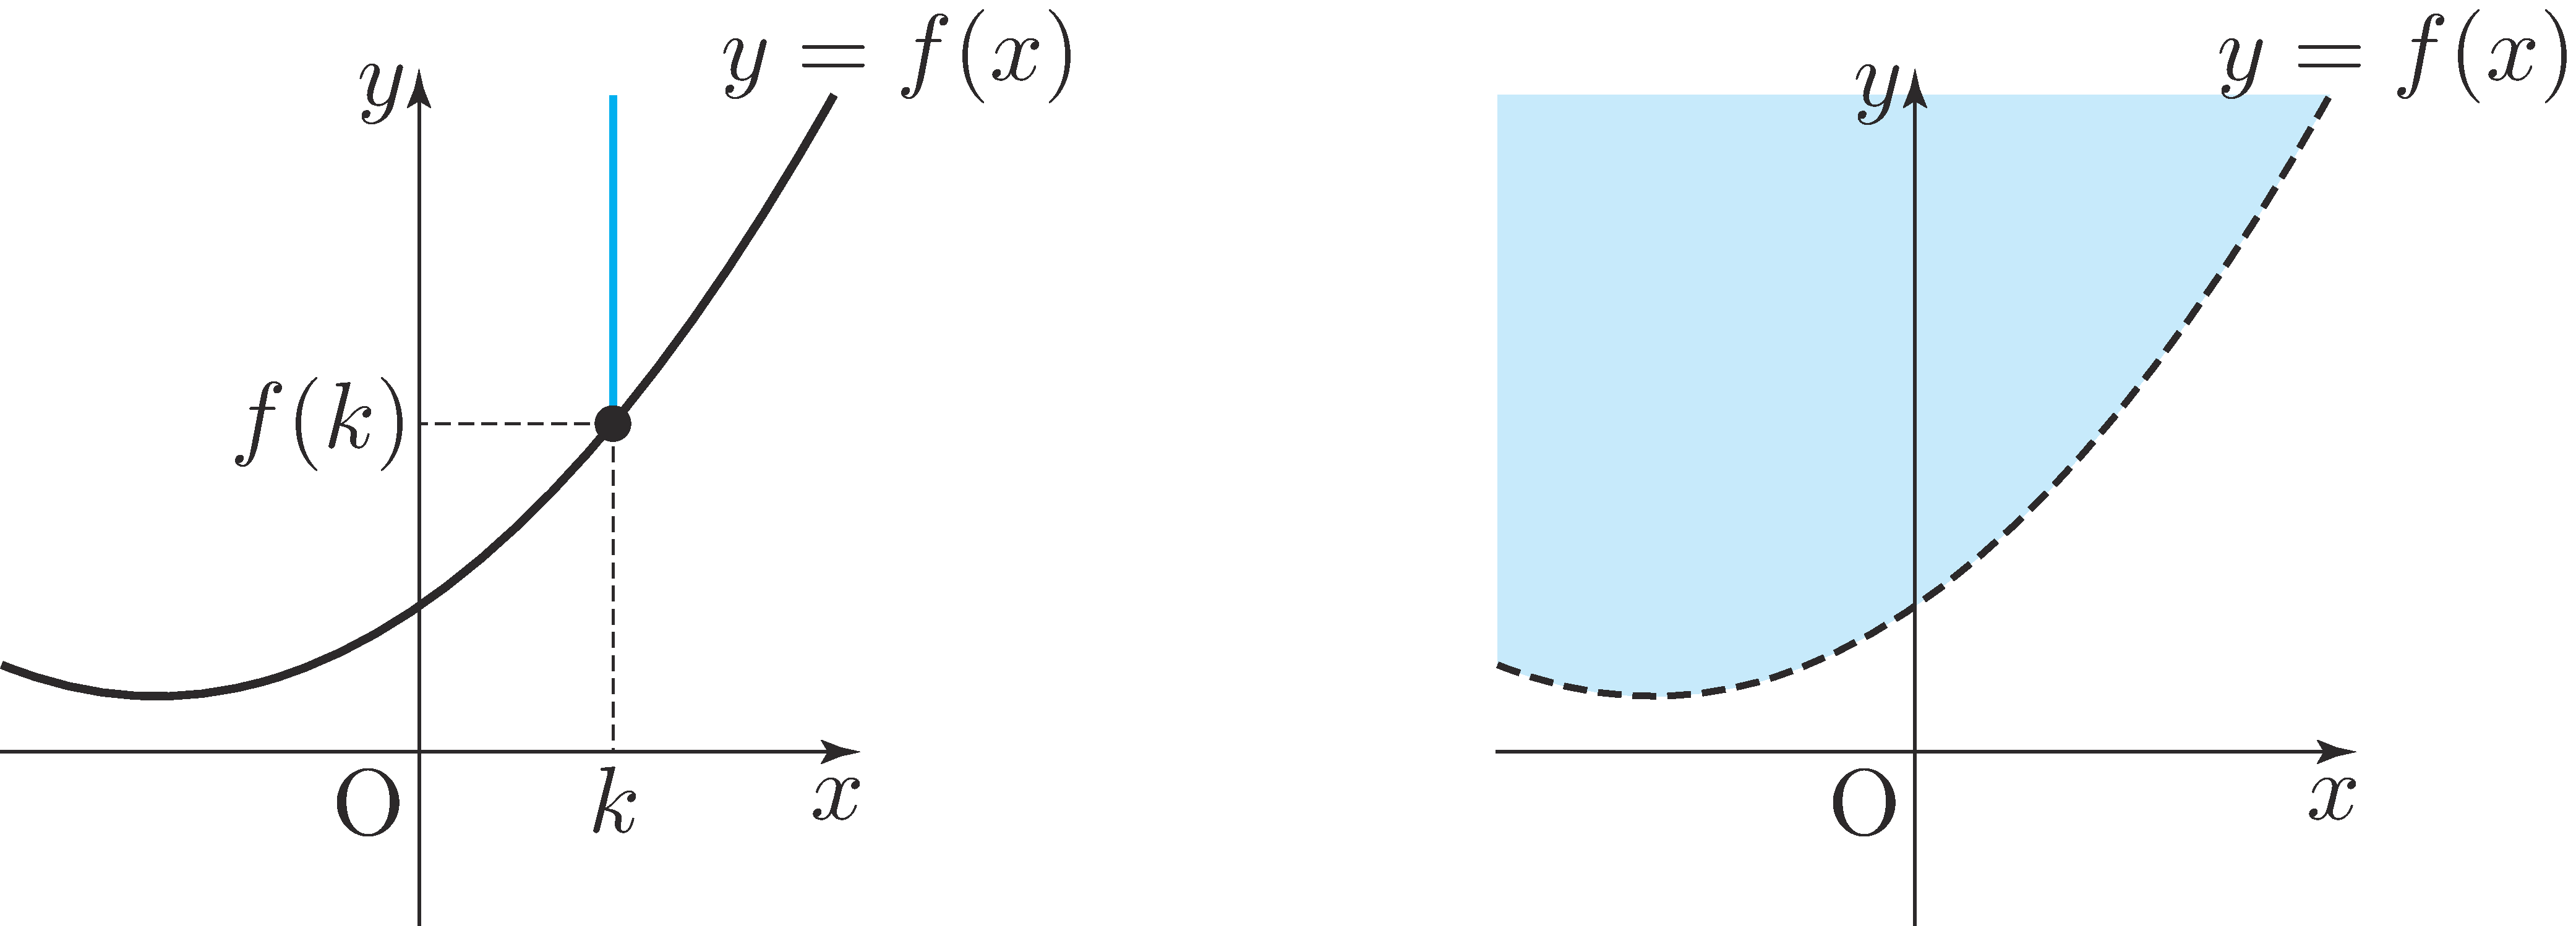
\includegraphics[scale=\pgfkeysvalueof{picsize}]{DBs/pic/zery_07.pdf}\
	\end{center}앞서 $y=f\left( x \right) $ 위의 점 $\xy{k}{f\left( k \right) }$가 $x$ 좌표는 $k$, $y$ 좌표는 $f\left( k \right) $인 점을 포함하는 것을 배웠습니다. $y>f\left( x \right) $라면, $x$좌표가 $k$일 때, $y$좌표가 $f\left( k \right) $보다 큰 점들을 의미하게 됩니다. 이러한 점이 나타내는 도형은 왼쪽 그림에서의 색칠된 직선과 같습니다. 정의역에 속하는 모든 실수 $x$에 대하여 같은 방법으로 해석하면, 오른쪽 그림과 같이 곡선 위쪽 영역을 모두 색칠하게 됩니다. 이때 $y=f\left( x \right) $는 부등식의 영역에 포함되지 않으므로 점선으로 그려줍니다. 
\begin{center} 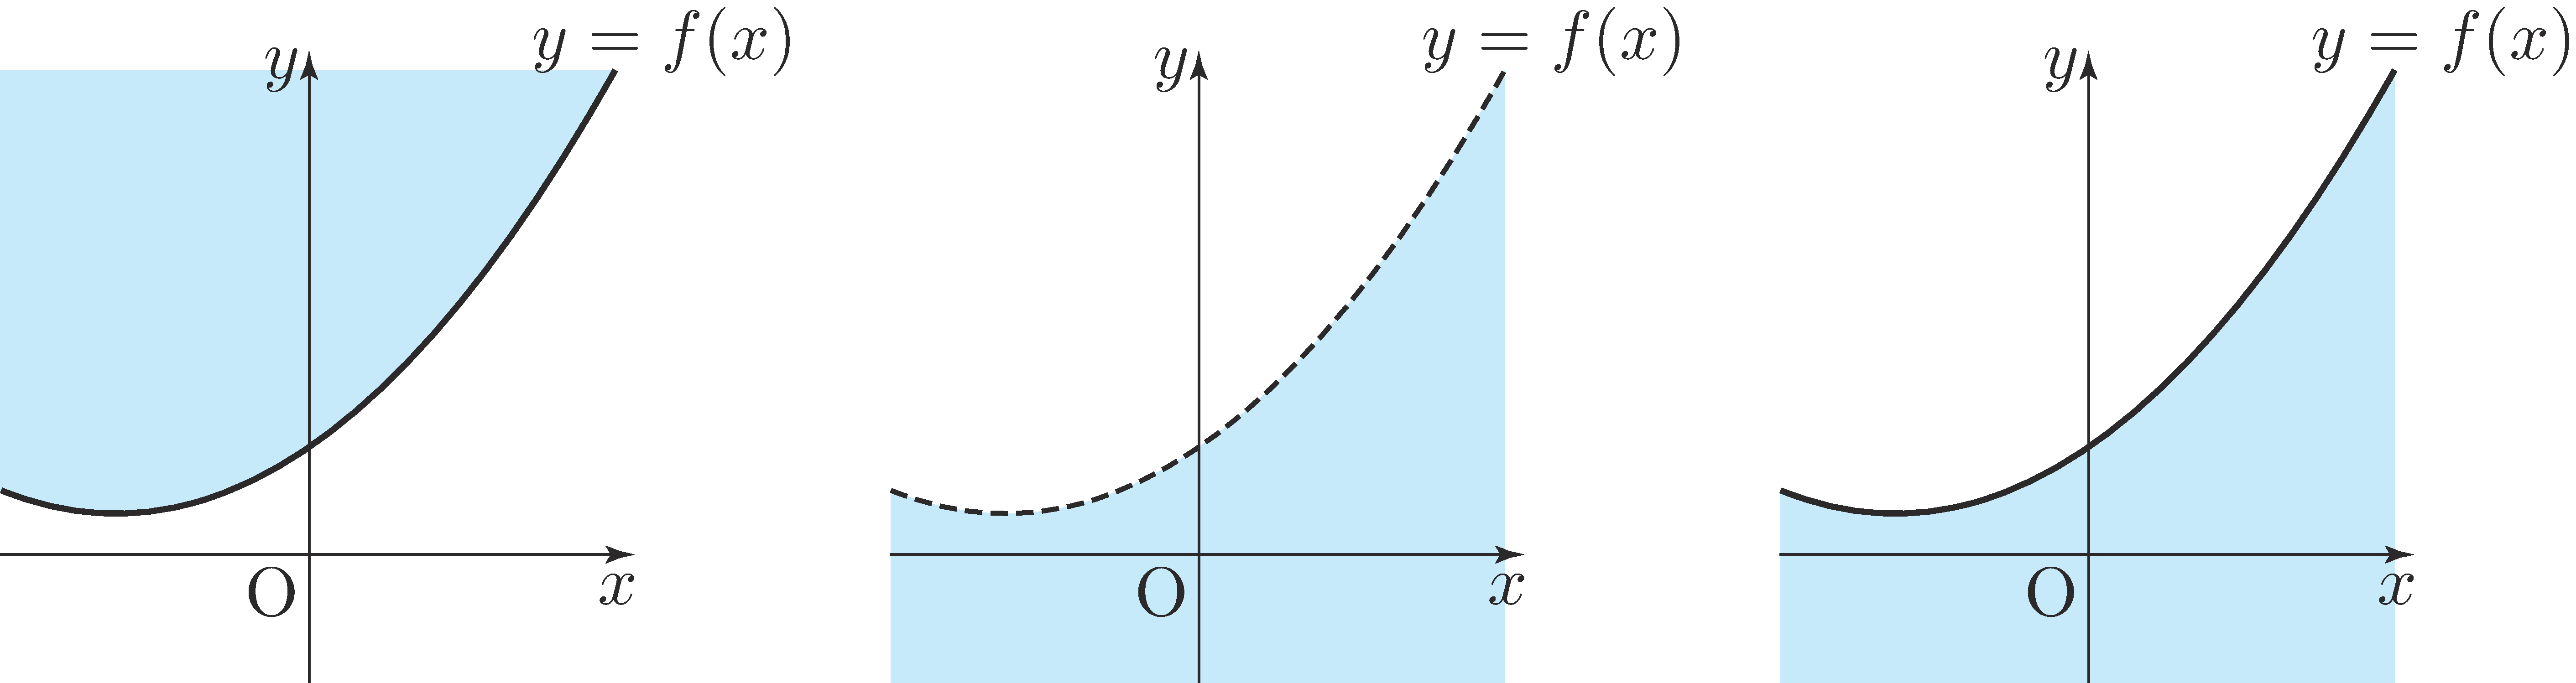
\includegraphics[scale=\pgfkeysvalueof{picsize}]{DBs/pic/zery_07_1.pdf}\
	\end{center}같은 방법으로 $y \ge f\left( x \right) $, $y<f\left( x \right) $, $y \le f\left( x \right) $가 나타내는 영역을 차례대로 표시하면 각각 위 그림과 같습니다.

\section{부등식의 영역}\term{부등식의 영역}{0}\begin{center}
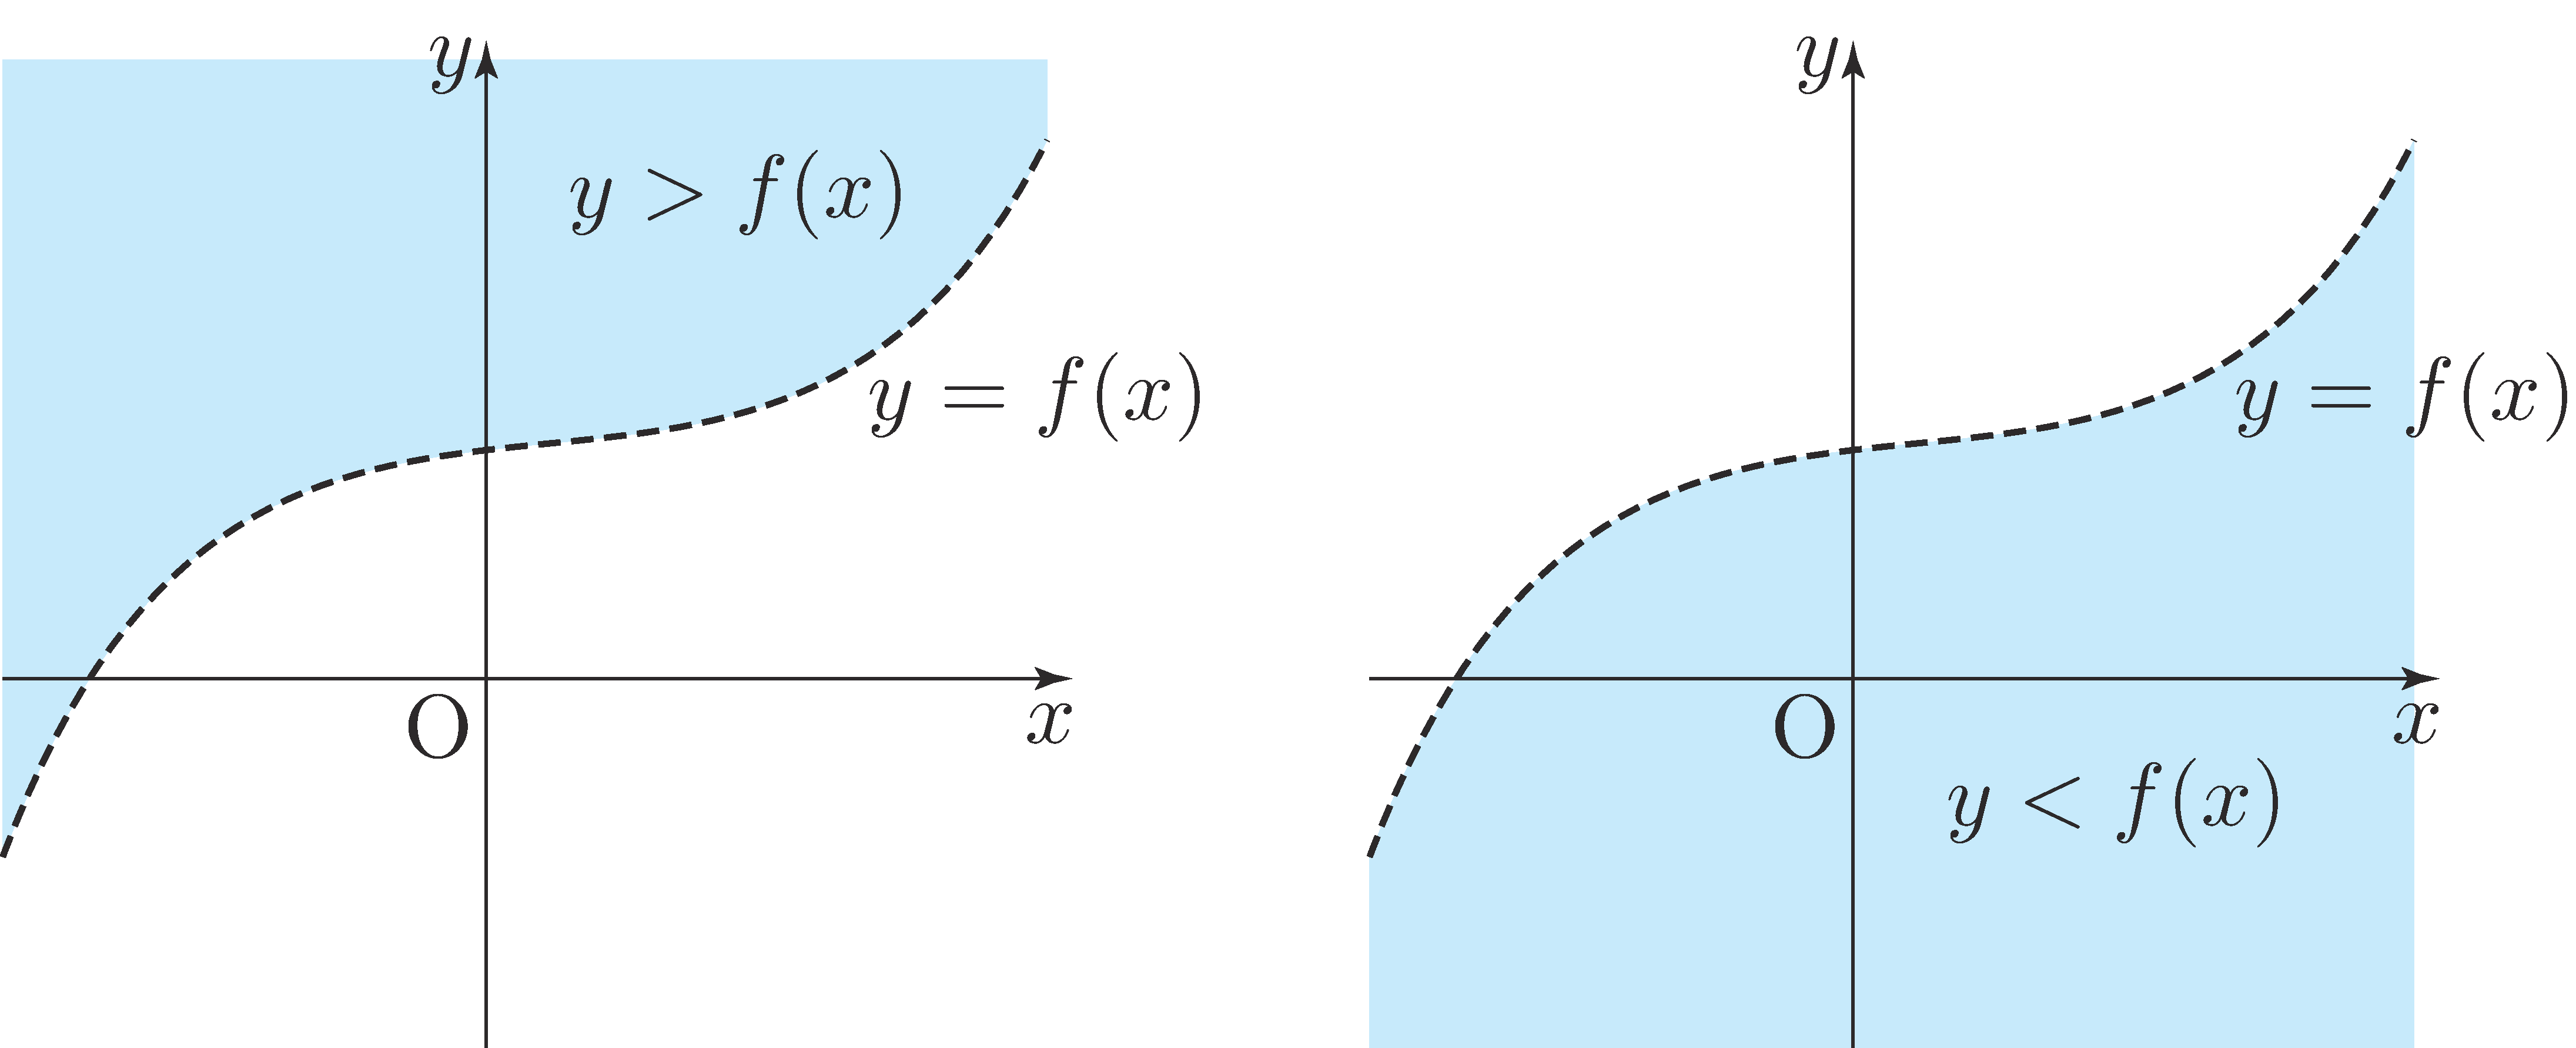
\includegraphics[scale=0.115]{pic0/pic151.pdf}\
\end{center}좌표평면에서 부등식 $y>f(x)$의 영역은 곡선 $y=f(x)$의 윗부분(위쪽)이고, 부등식 $y<f(x)$의 영역은 아랫부분(아래쪽)입니다. 부등식에 등호가 포함되어 있으면 곡선 $y=f(x)$도 포함하며, 영역의 경계선인 곡선을 실선으로 나타냅니다. 부등식 등호가 포함되어 있지 않으면 곡선 $y=f(x)$를 포함하지 않으며, 영역의 경계선인 곡선을 점선으로 나타냅니다.
\begin{center}
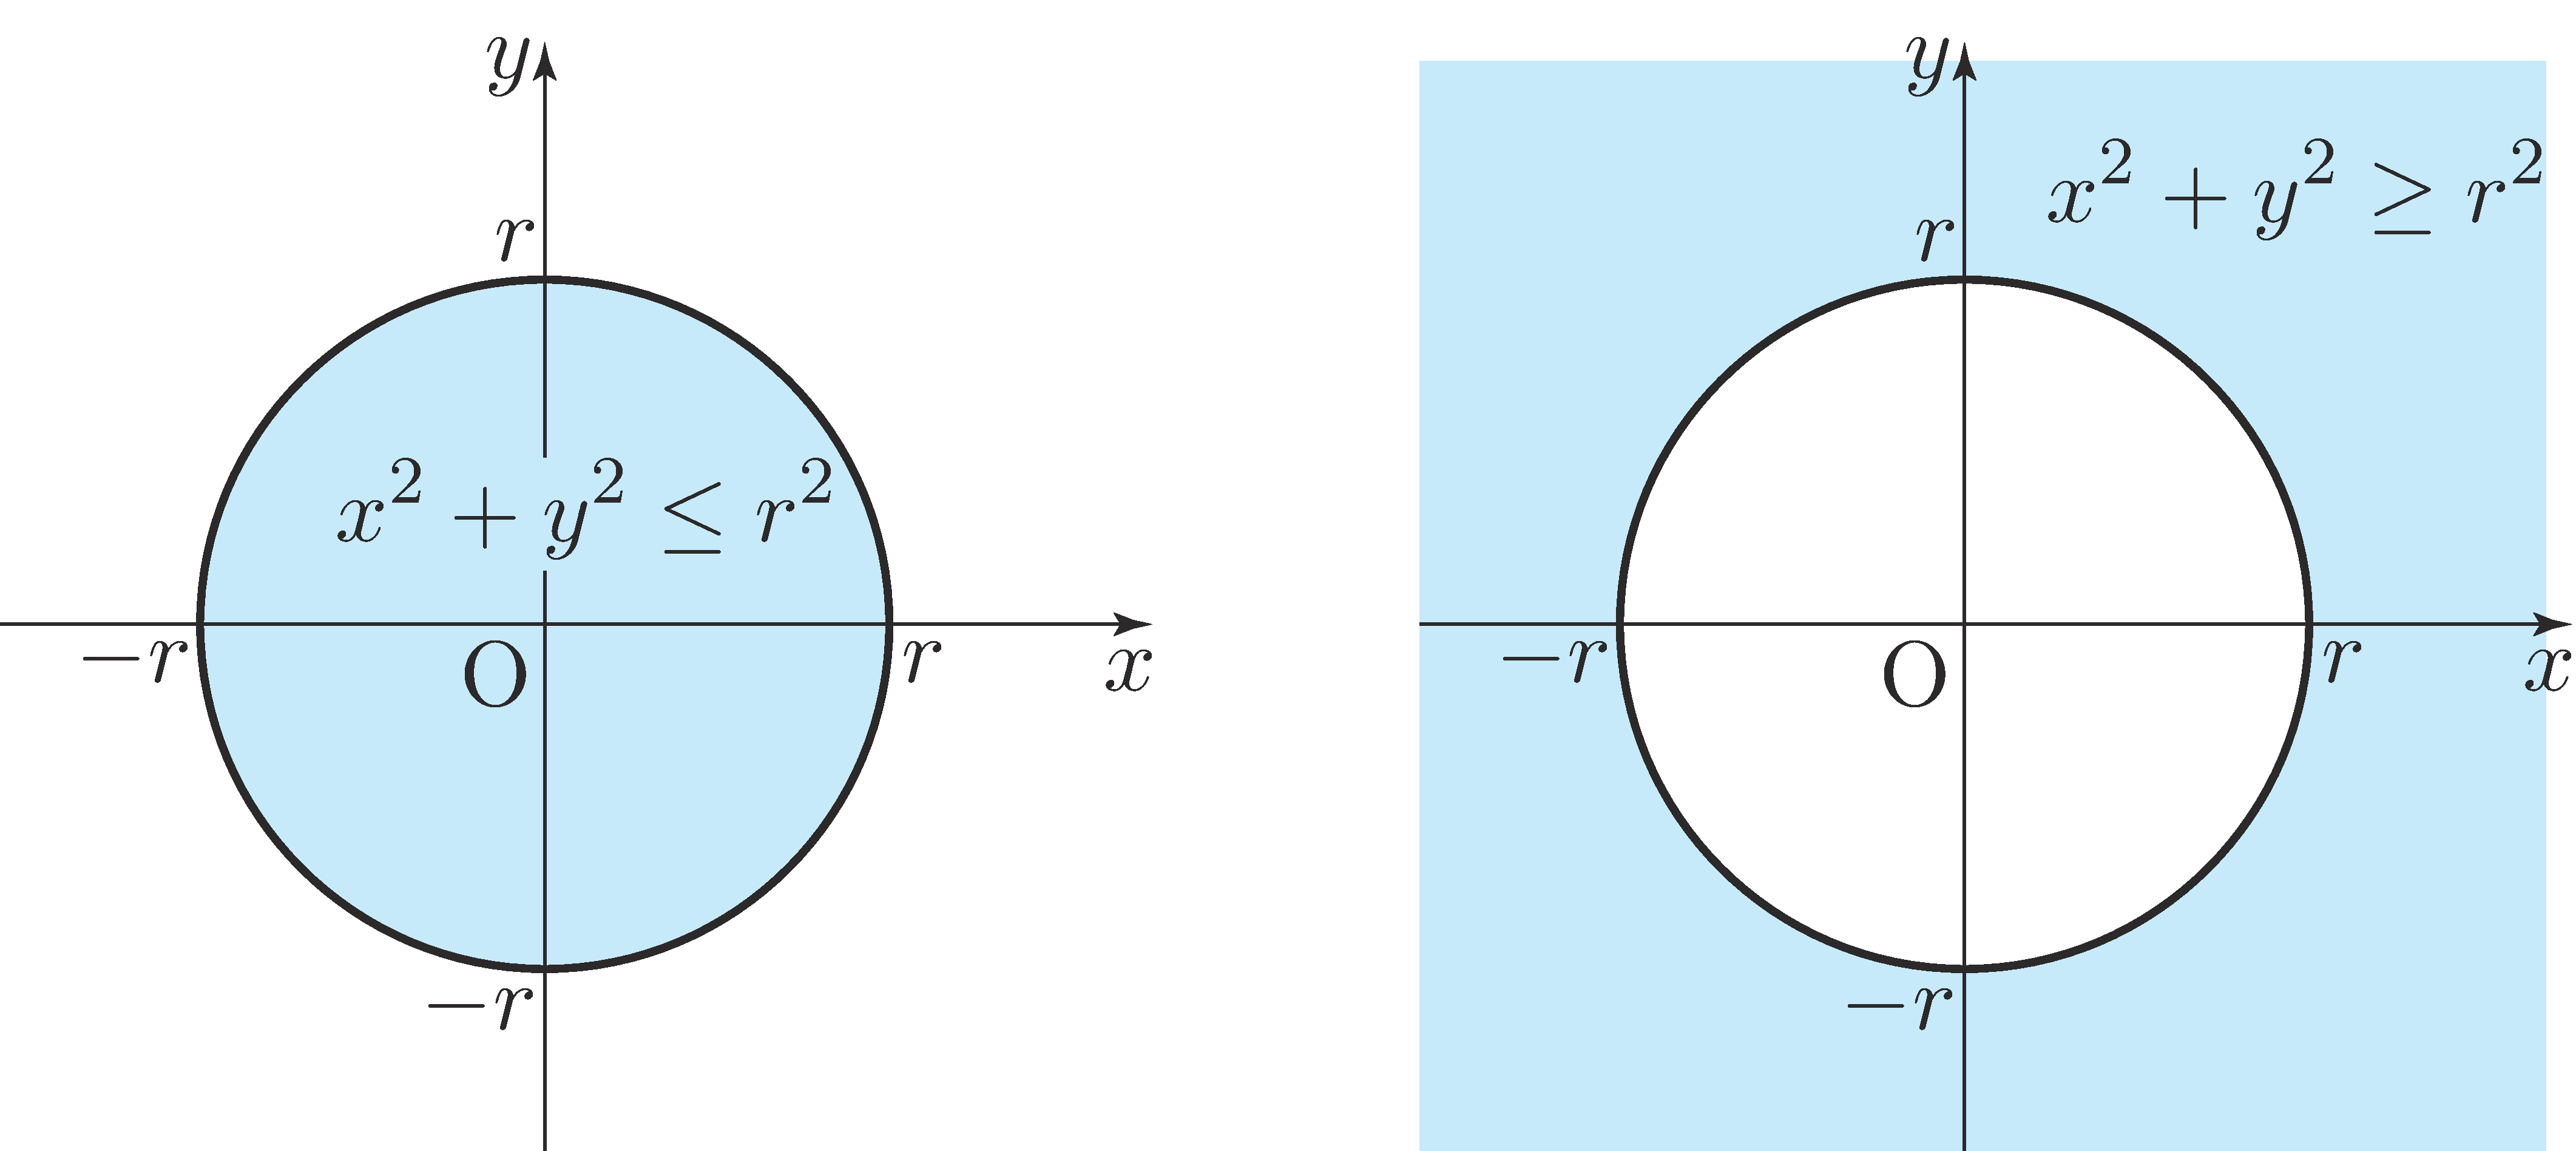
\includegraphics[scale=0.115]{pic0/pic152.pdf}\
\end{center}좌표평면에서 부등식 $x^2 + y^2 < r^2$의 영역은 원 $x^2 + y^2 = r^2$의 내부이고, 부등식 $x^2 + y^2 > r^2$의 영역은 원 $x^2 + y^2 = r^2$의 외부입니다.  부등식에 등호가 포함되어 있으면 원 $x^2 + y^2 = r^2$도 포함하며, 영역의 경계선인 원을 실선으로 나타냅니다. 부등식에 등호가 포함되어 있지 않으면 원 $x^2 + y^2 = r^2$을 포함하지 않으며 영역의 경계선인 원을 점선으로 나타냅니다.
\begin{figure}[h]
  \centering
  \subfloat[][]{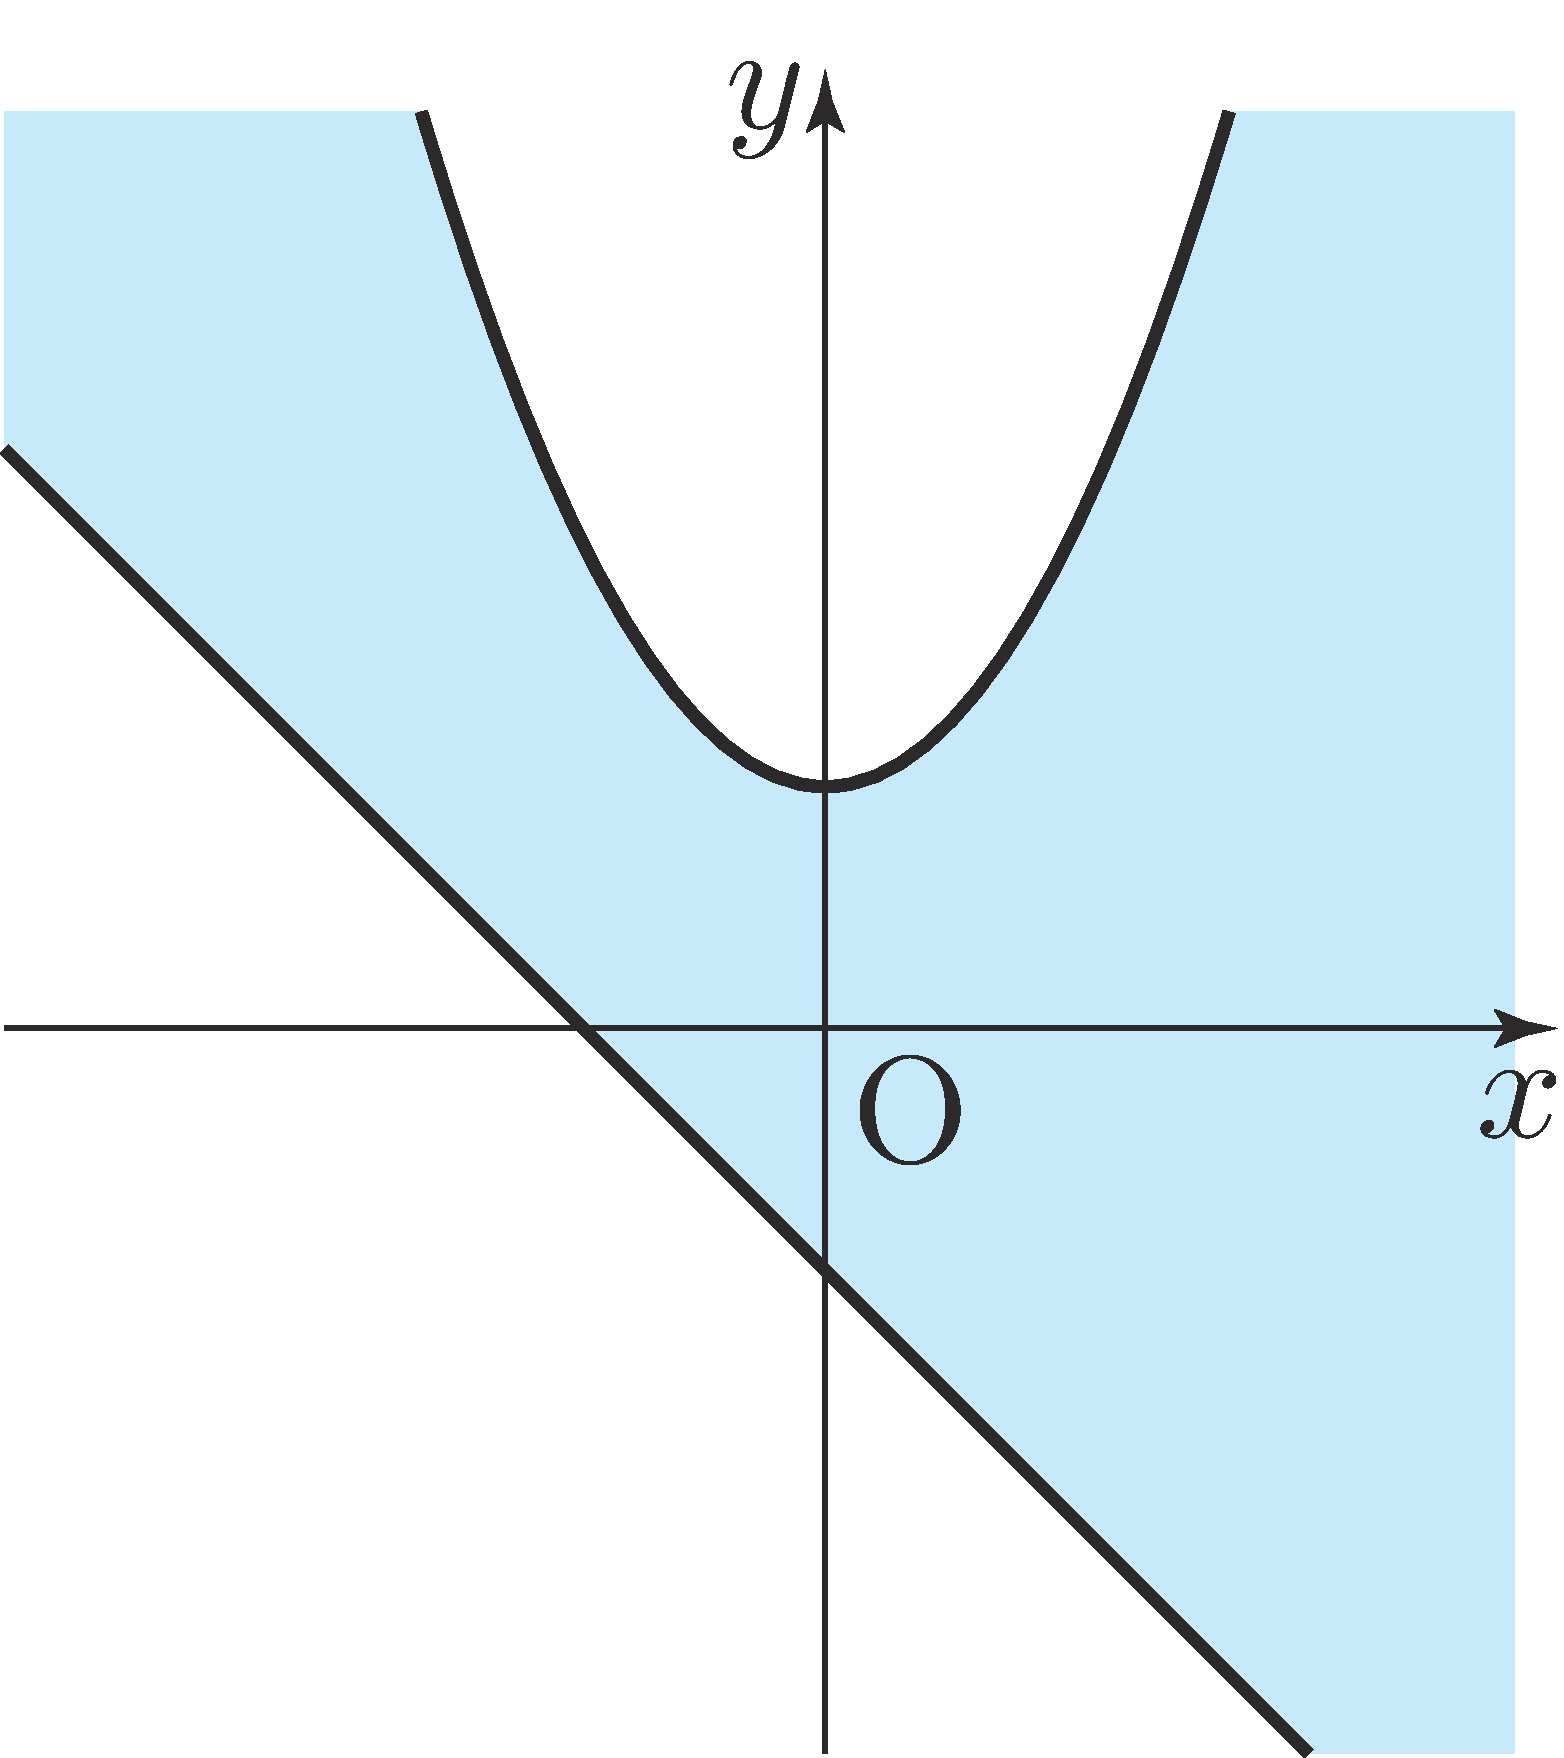
\includegraphics[scale=.115]{pic0/pic153_1.pdf}}
  \qquad
  \subfloat[][]{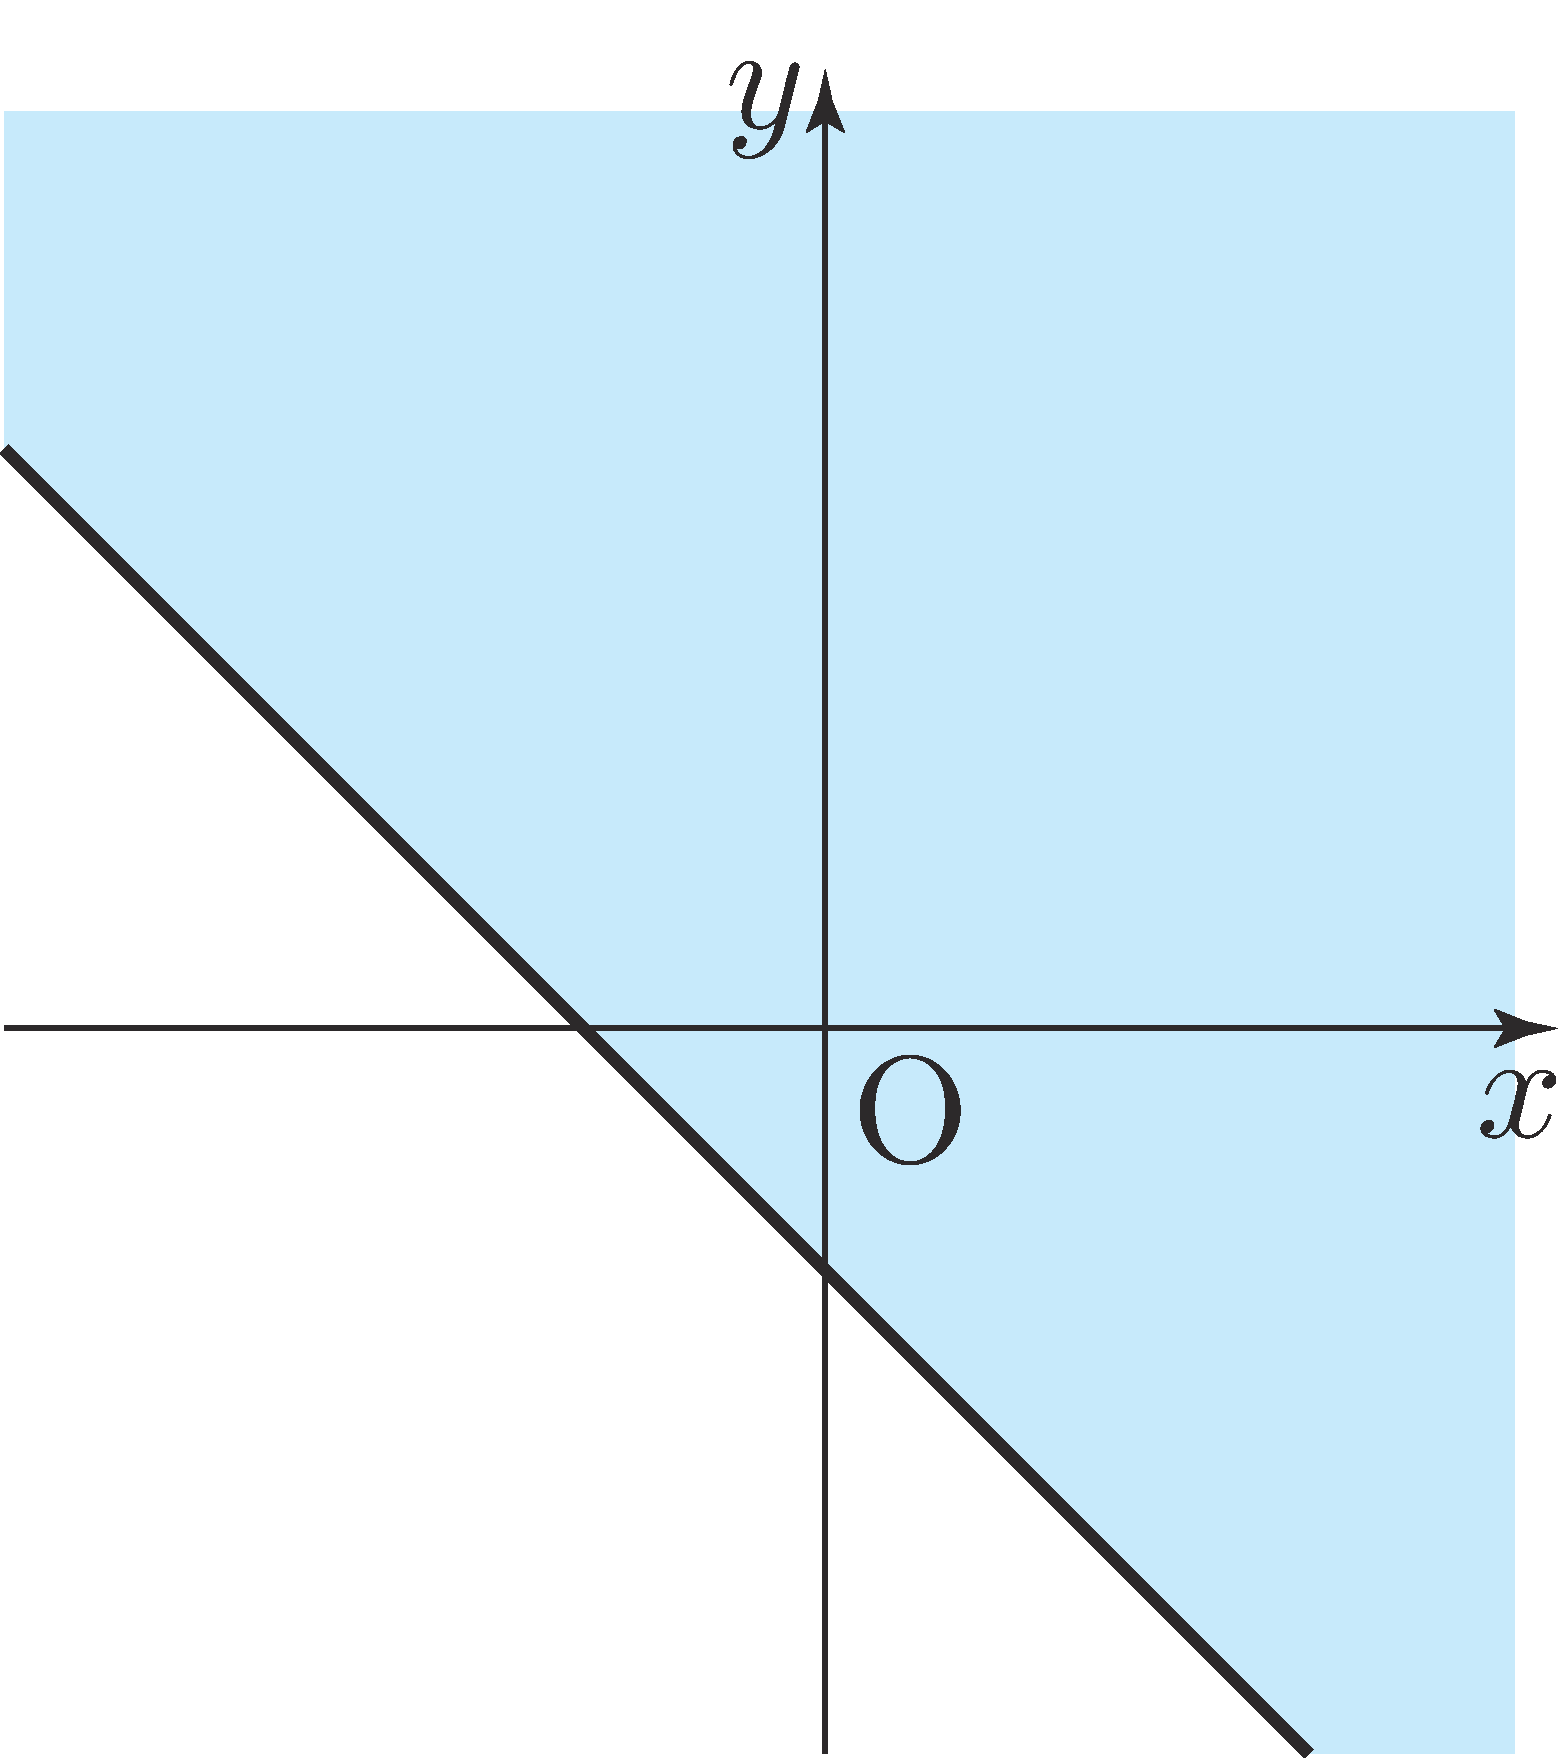
\includegraphics[scale=.115]{pic0/pic153_2.pdf}}
  \qquad
  \subfloat[][]{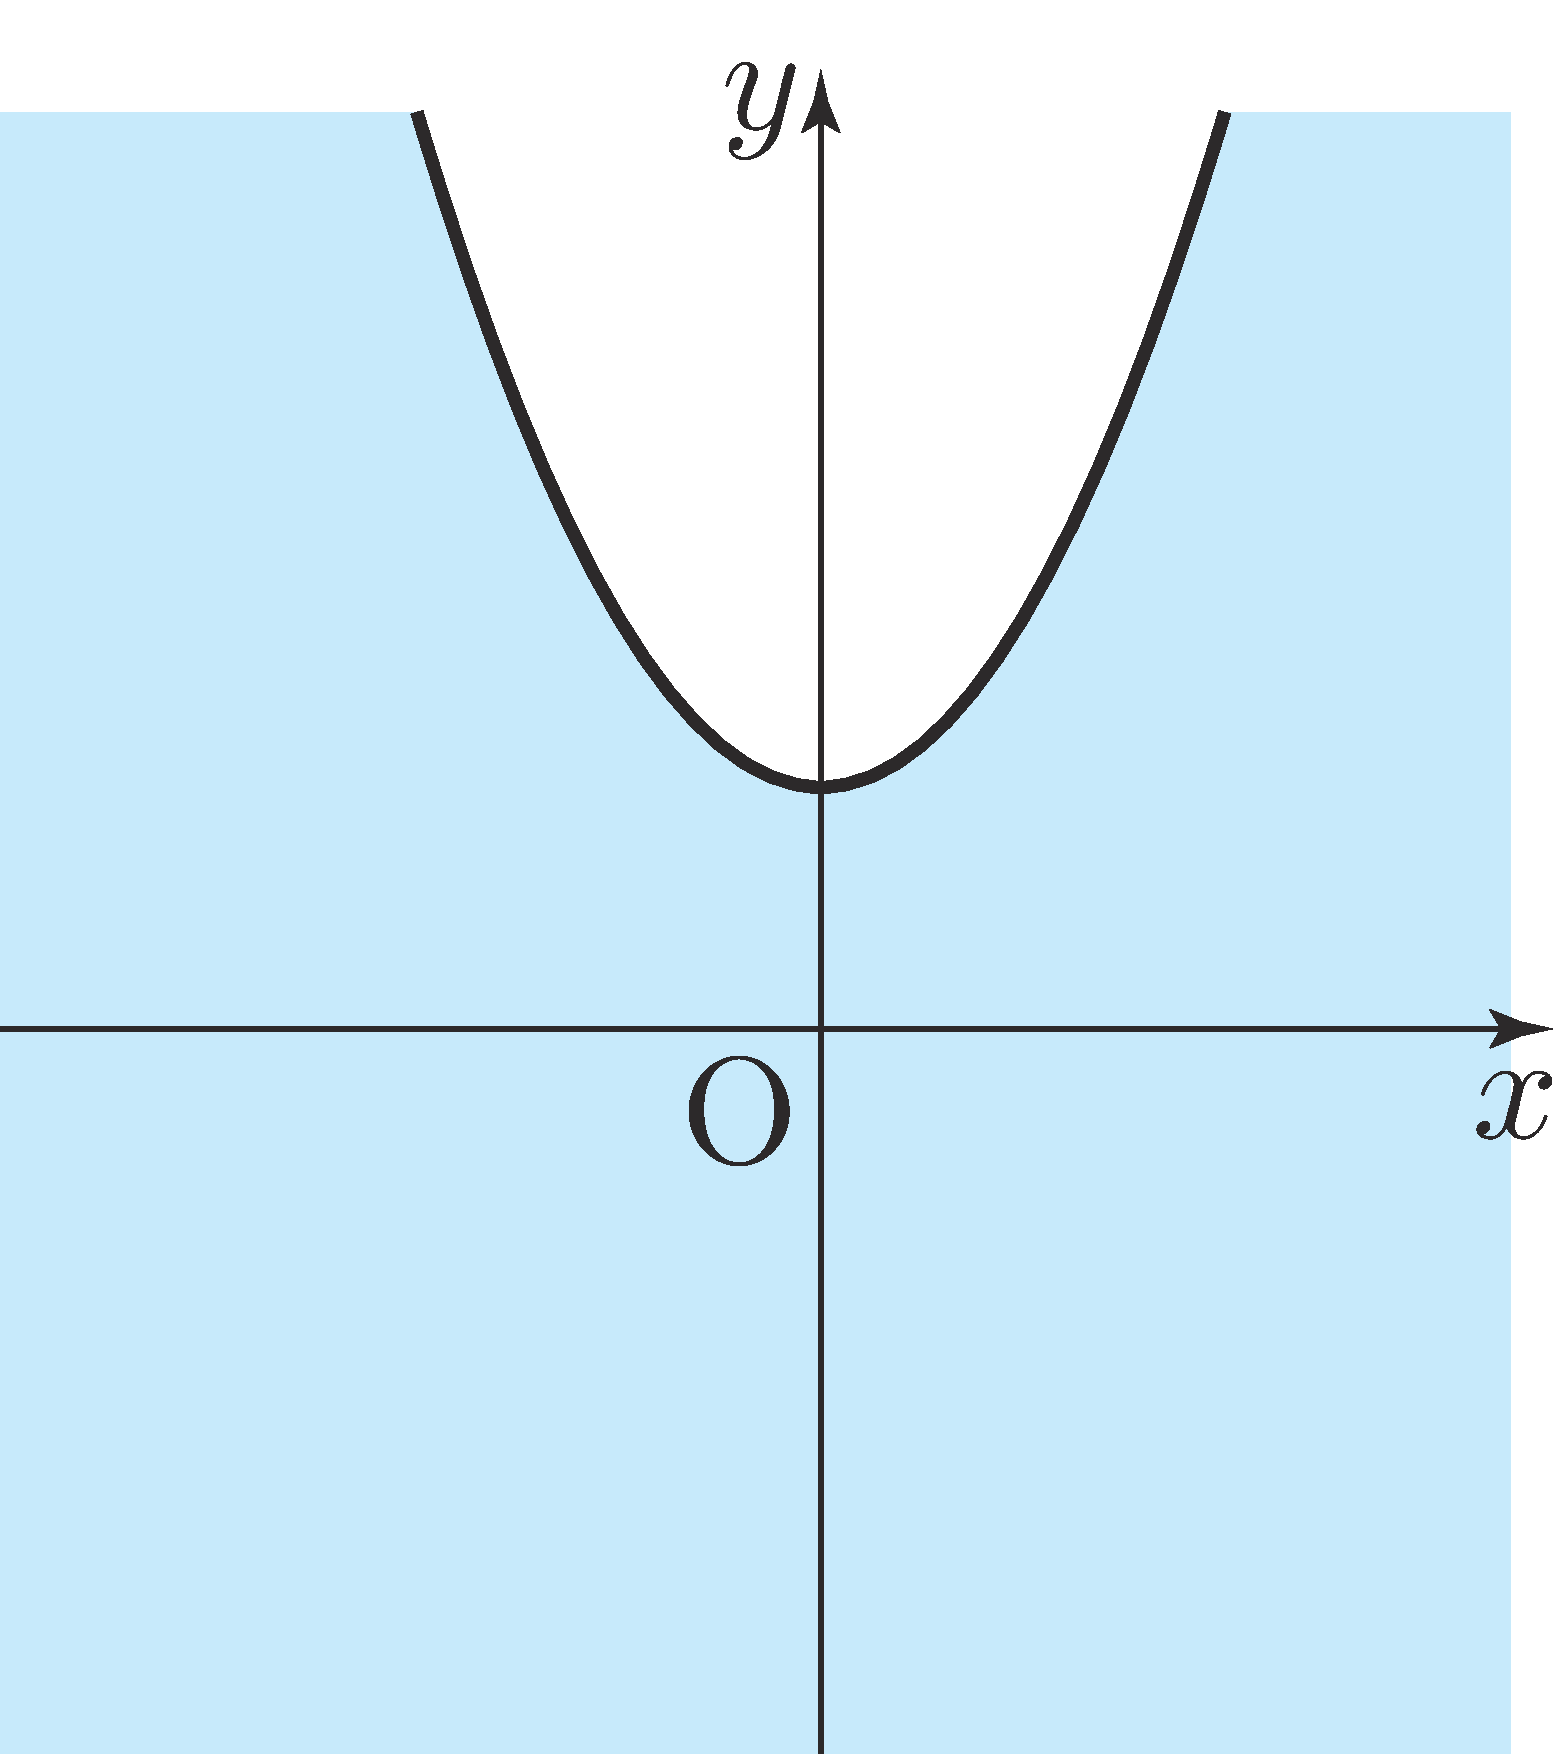
\includegraphics[scale=.115]{pic0/pic153_3.pdf}}
\end{figure}


연립부등식의 영역은 연립된 각각의 부등식의 영역의 공통 영역입니다. 예를 들어 연립부등식 \( \begin{cases}
x+y+1 \ge 0 \\[-.2em]
x^2 + 1 \ge y\end{cases}\)가 나타내는 영역은 (a)와 같은데, 이는 (b)에서 색칠된 영역인 $x+y+1 \ge 0$와 (c)에서 색칠된 영역인 $x^2 + 1 \ge y$의 공통영역입니다. 


\mychapter{그래프를 다룰 때 주의해야 할 기본 요소}{그래프를 다룰 때 주의해야 할 기본 요소에 대하여 알아봅시다.}

\section{좌표축과 원점}
\begin{center} 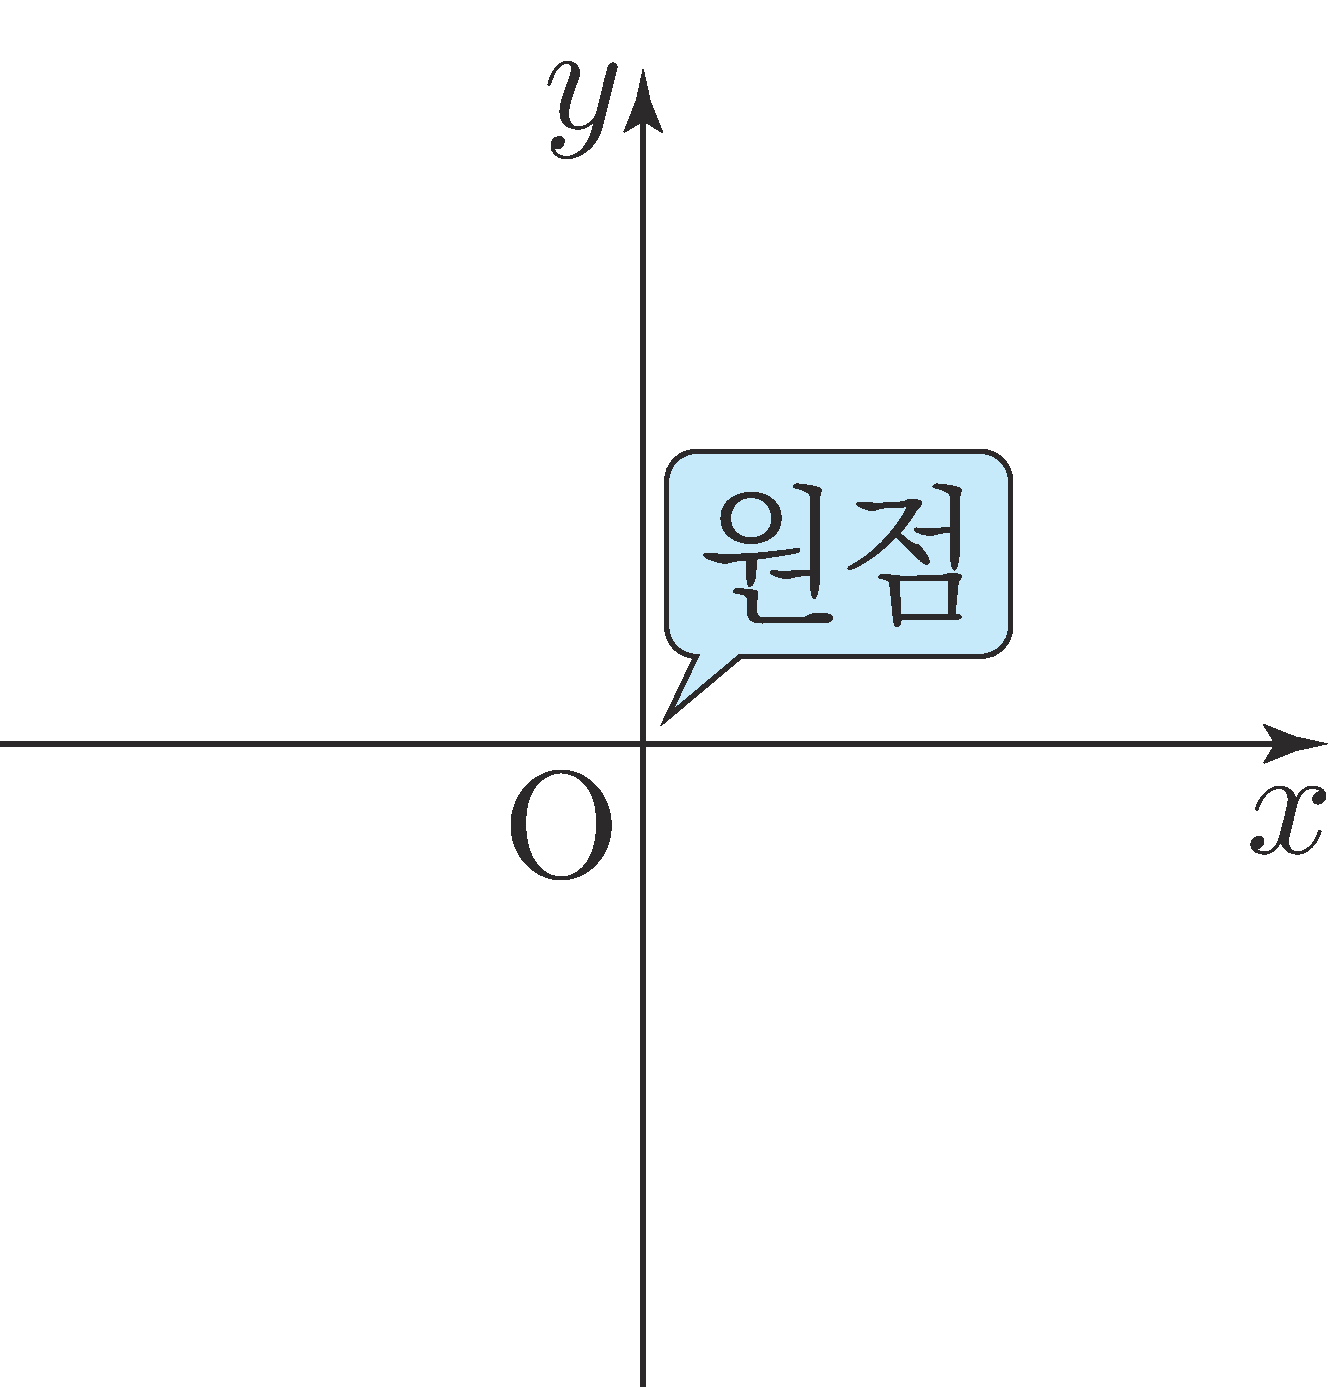
\includegraphics[scale=\pgfkeysvalueof{picsize}]{DBs/pic/zery_08.pdf}\
	\end{center}좌표축과 원점은 그래프가 그려질 무대인 좌표평면에 기본적으로 주어진 핵심정보라는 점에서 중요합니다. 또한 각 축의 교점인 원점은 일종의 불변하는 고정점과 같은 역할을 하므로 언제나 활용될 수 있음을 유념해야 합니다.

\section{좌표축에 수직인 직선}
\begin{center}
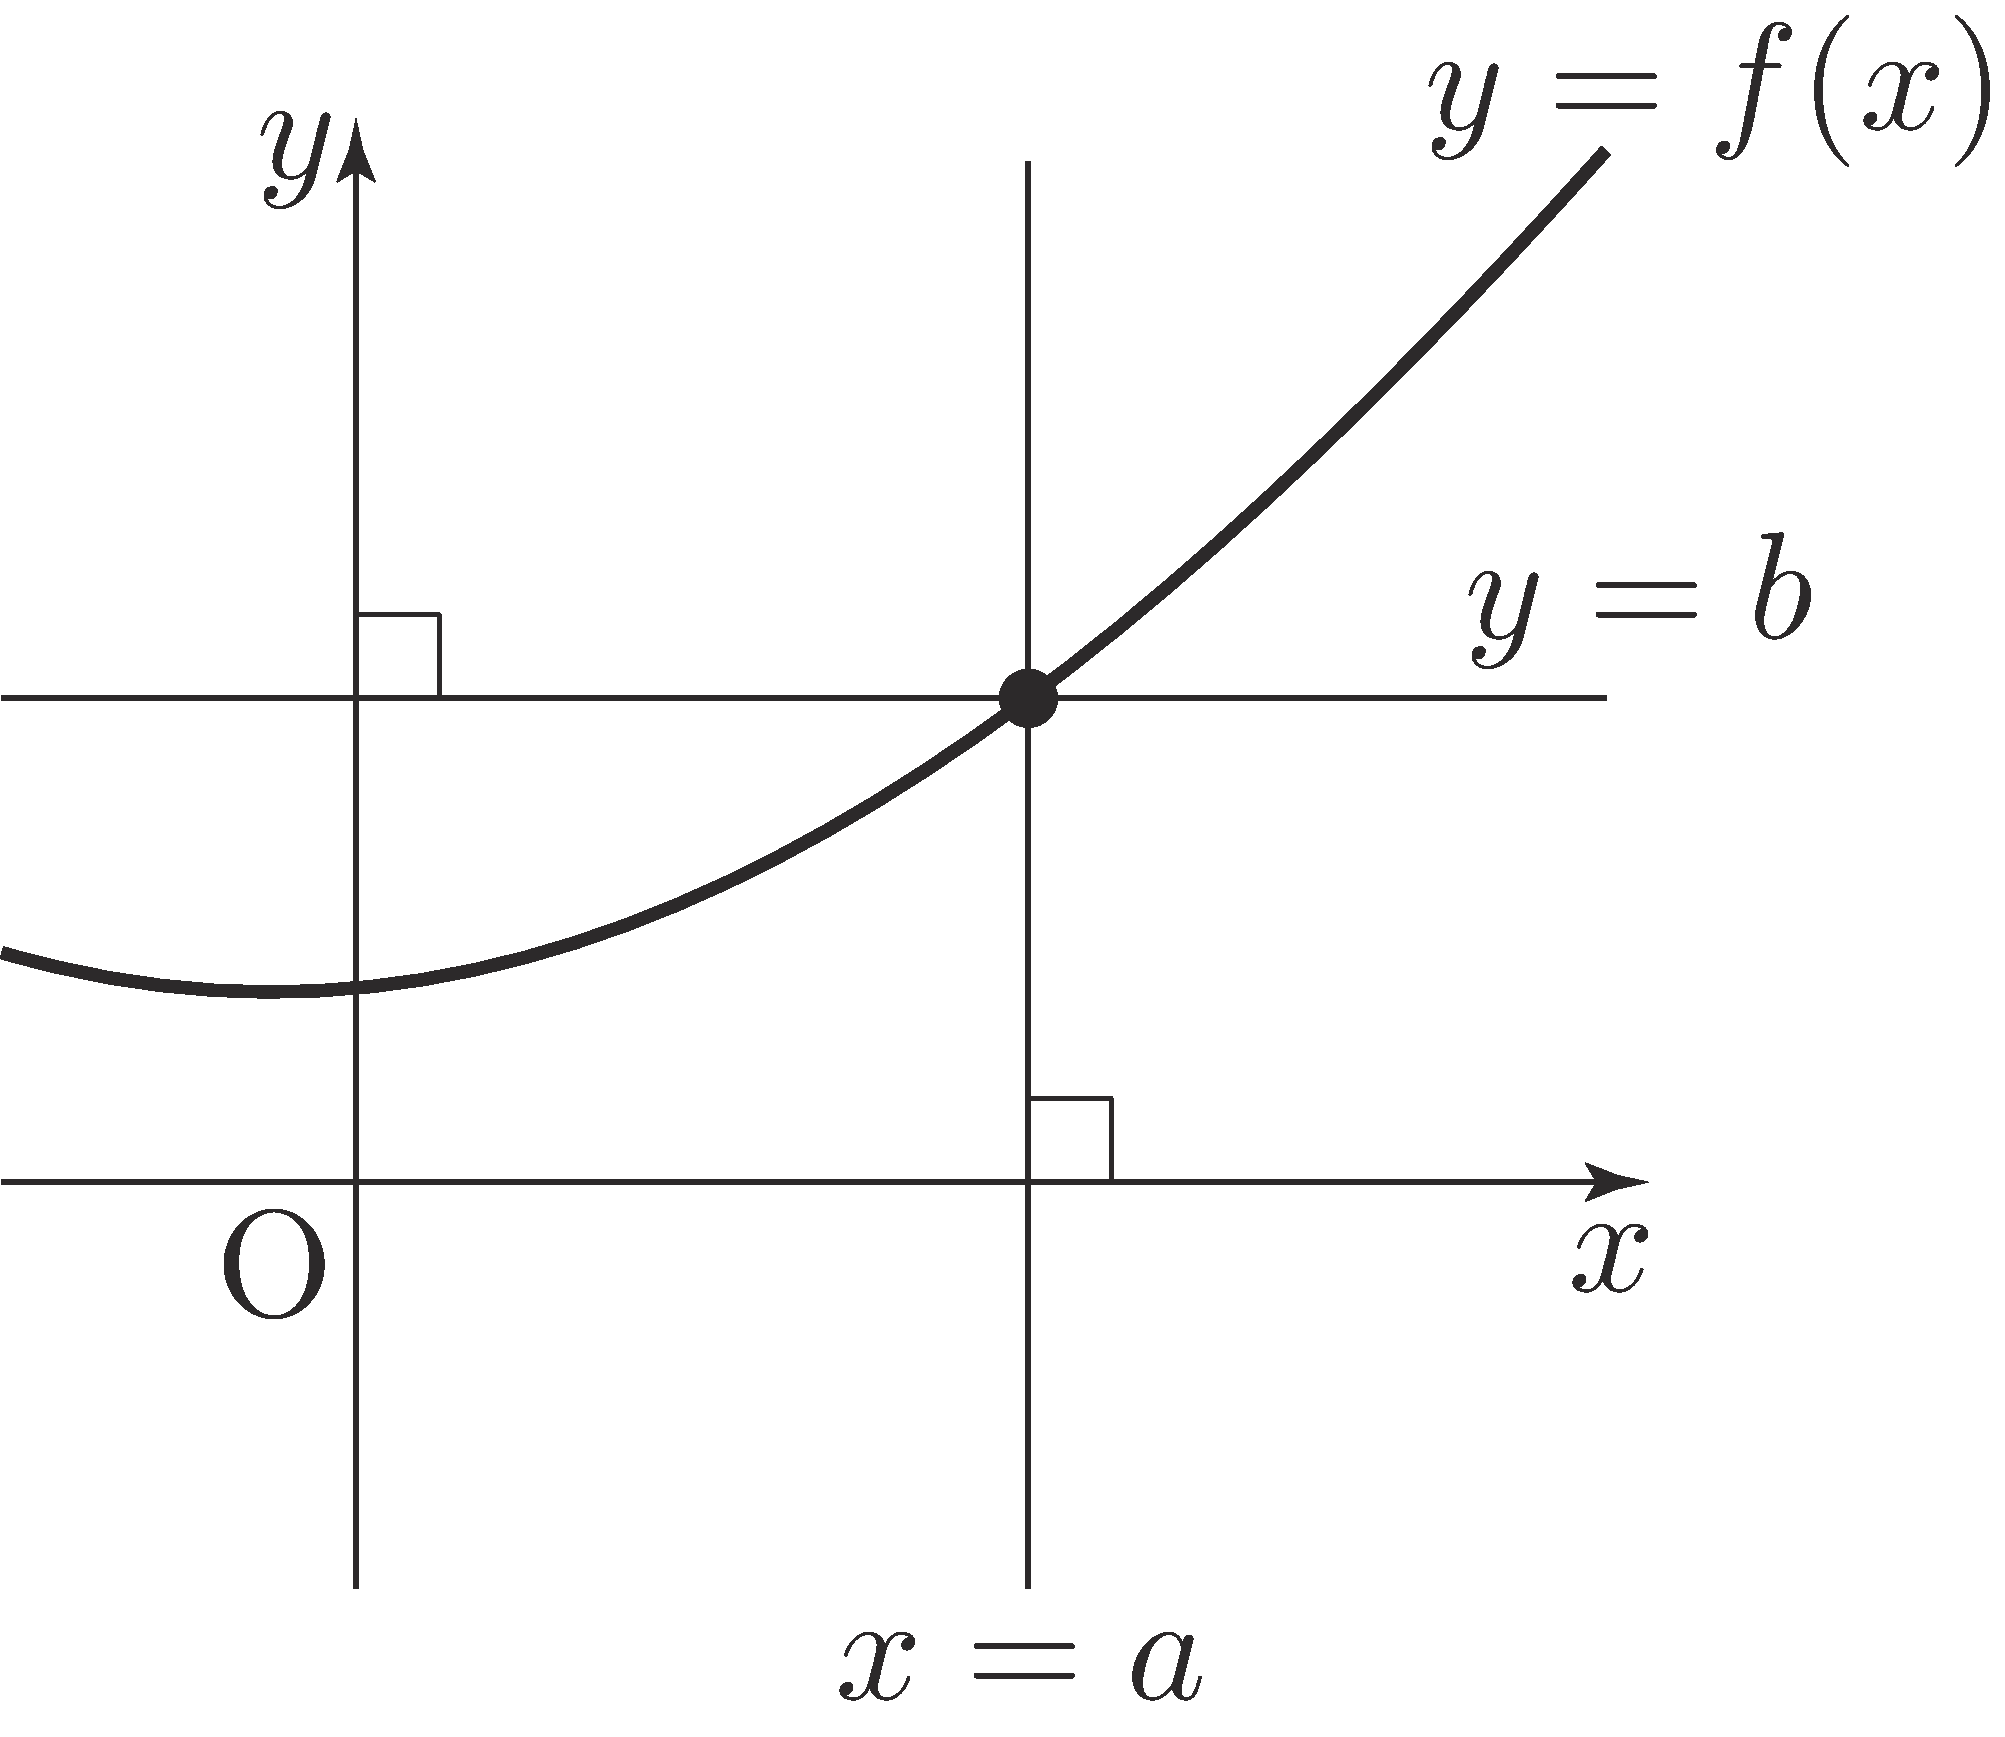
\includegraphics[scale=.125]{pic0/pic169.pdf}
  \end{center}좌표평면에서 `좌표'의 정의를 생각해보면, 각 좌표축에 수직인 두 직선이 각 좌표축과 만나는 점을 이용하여 정의됩니다. 따라서 각 축에 수직인 직선을 생각하는 것은 자연스럽습니다. 좌표를 정의할 때의 사고과정과 동일하기 때문입니다.
\begin{center}
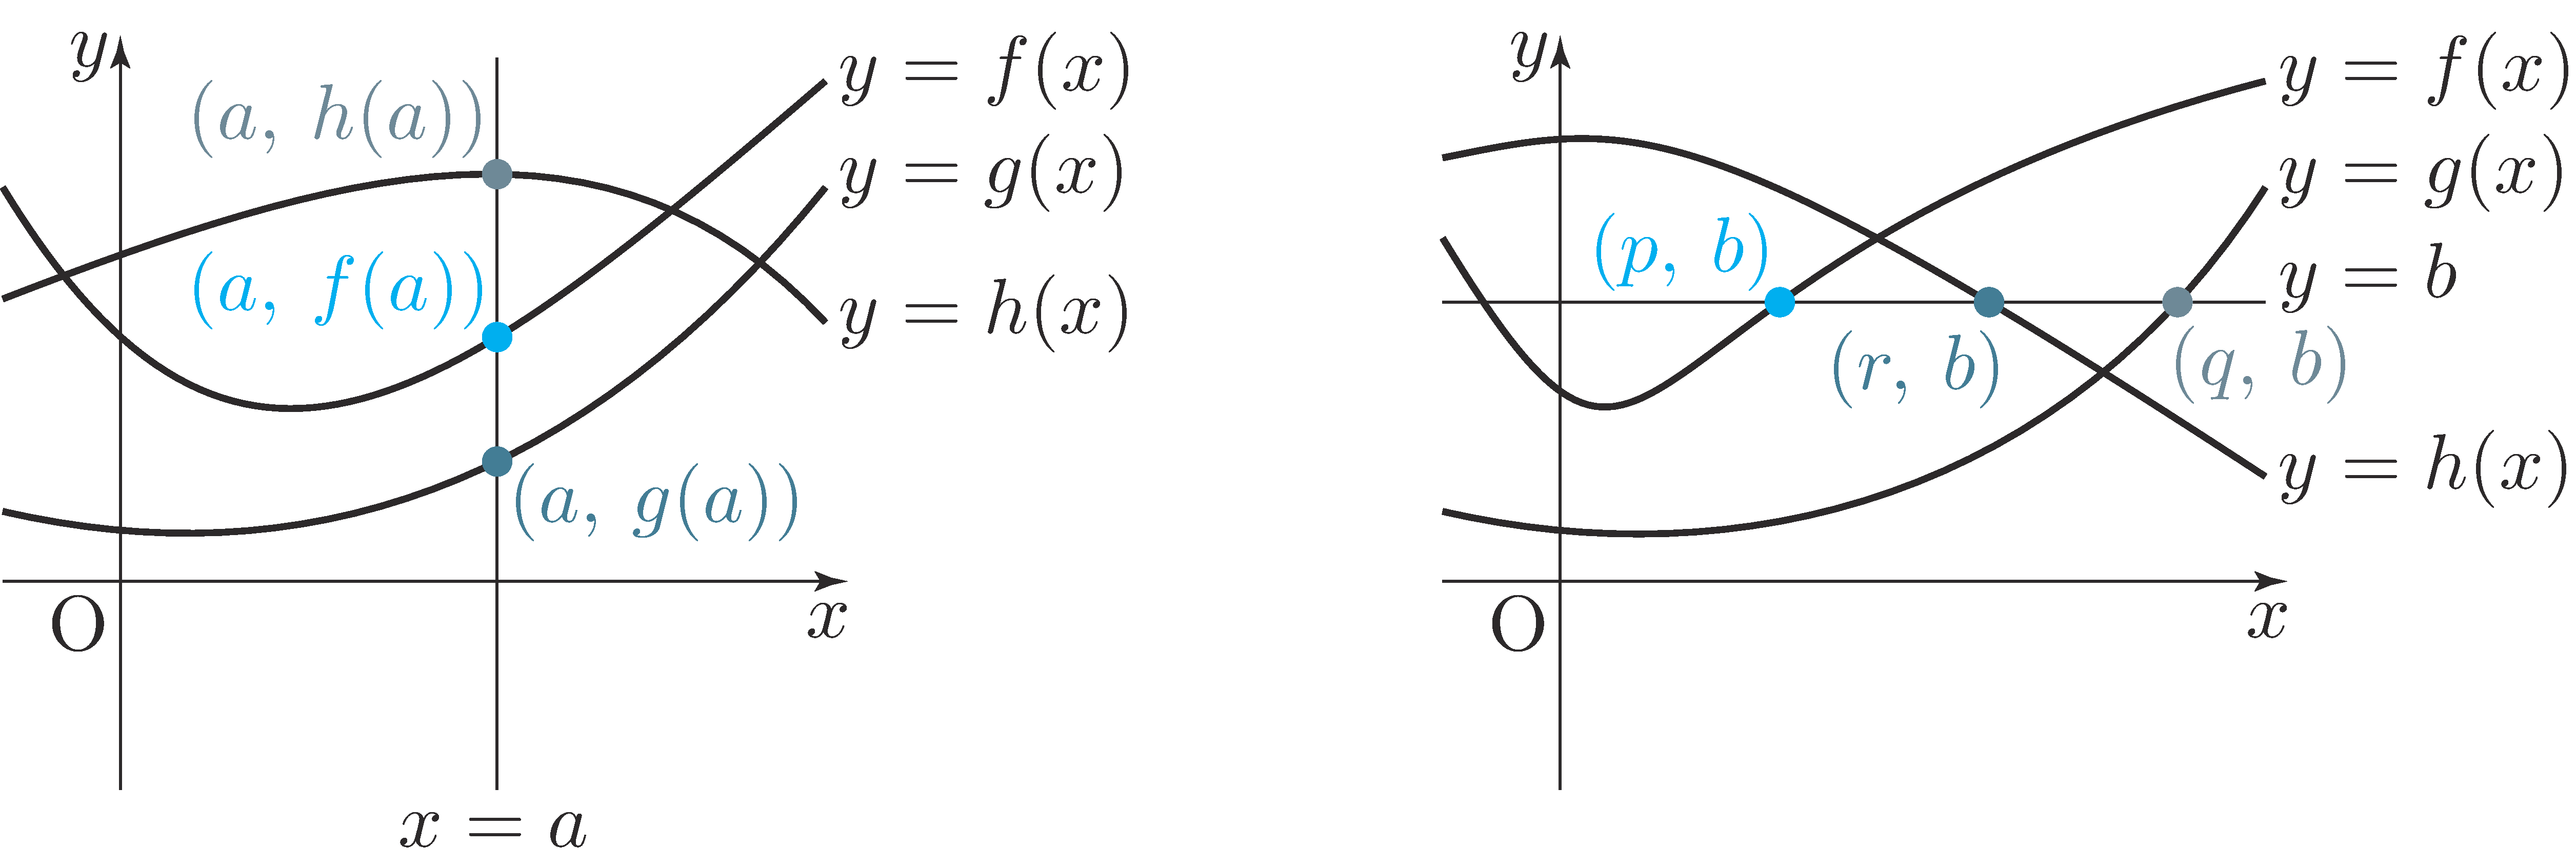
\includegraphics[scale=.125]{pic0/pic170.pdf}
  \end{center}또한 $x$축에 수직인 직선 위의 점들은 $x$좌표가 같은 점들을 나타내고, $y$축에 수직인 직선 위의 점들은 $y$좌표가 같은 점들을 나타내므로, `$x$좌표가 같은 점', `$y$좌표가 같은 점'과 같은 조건이 주어졌을 때 좌표축에 수직인 직선이 유용하게 쓰일 수 있음을 알 수 있습니다. 
\clearpage
\section{정의역}
\begin{center} 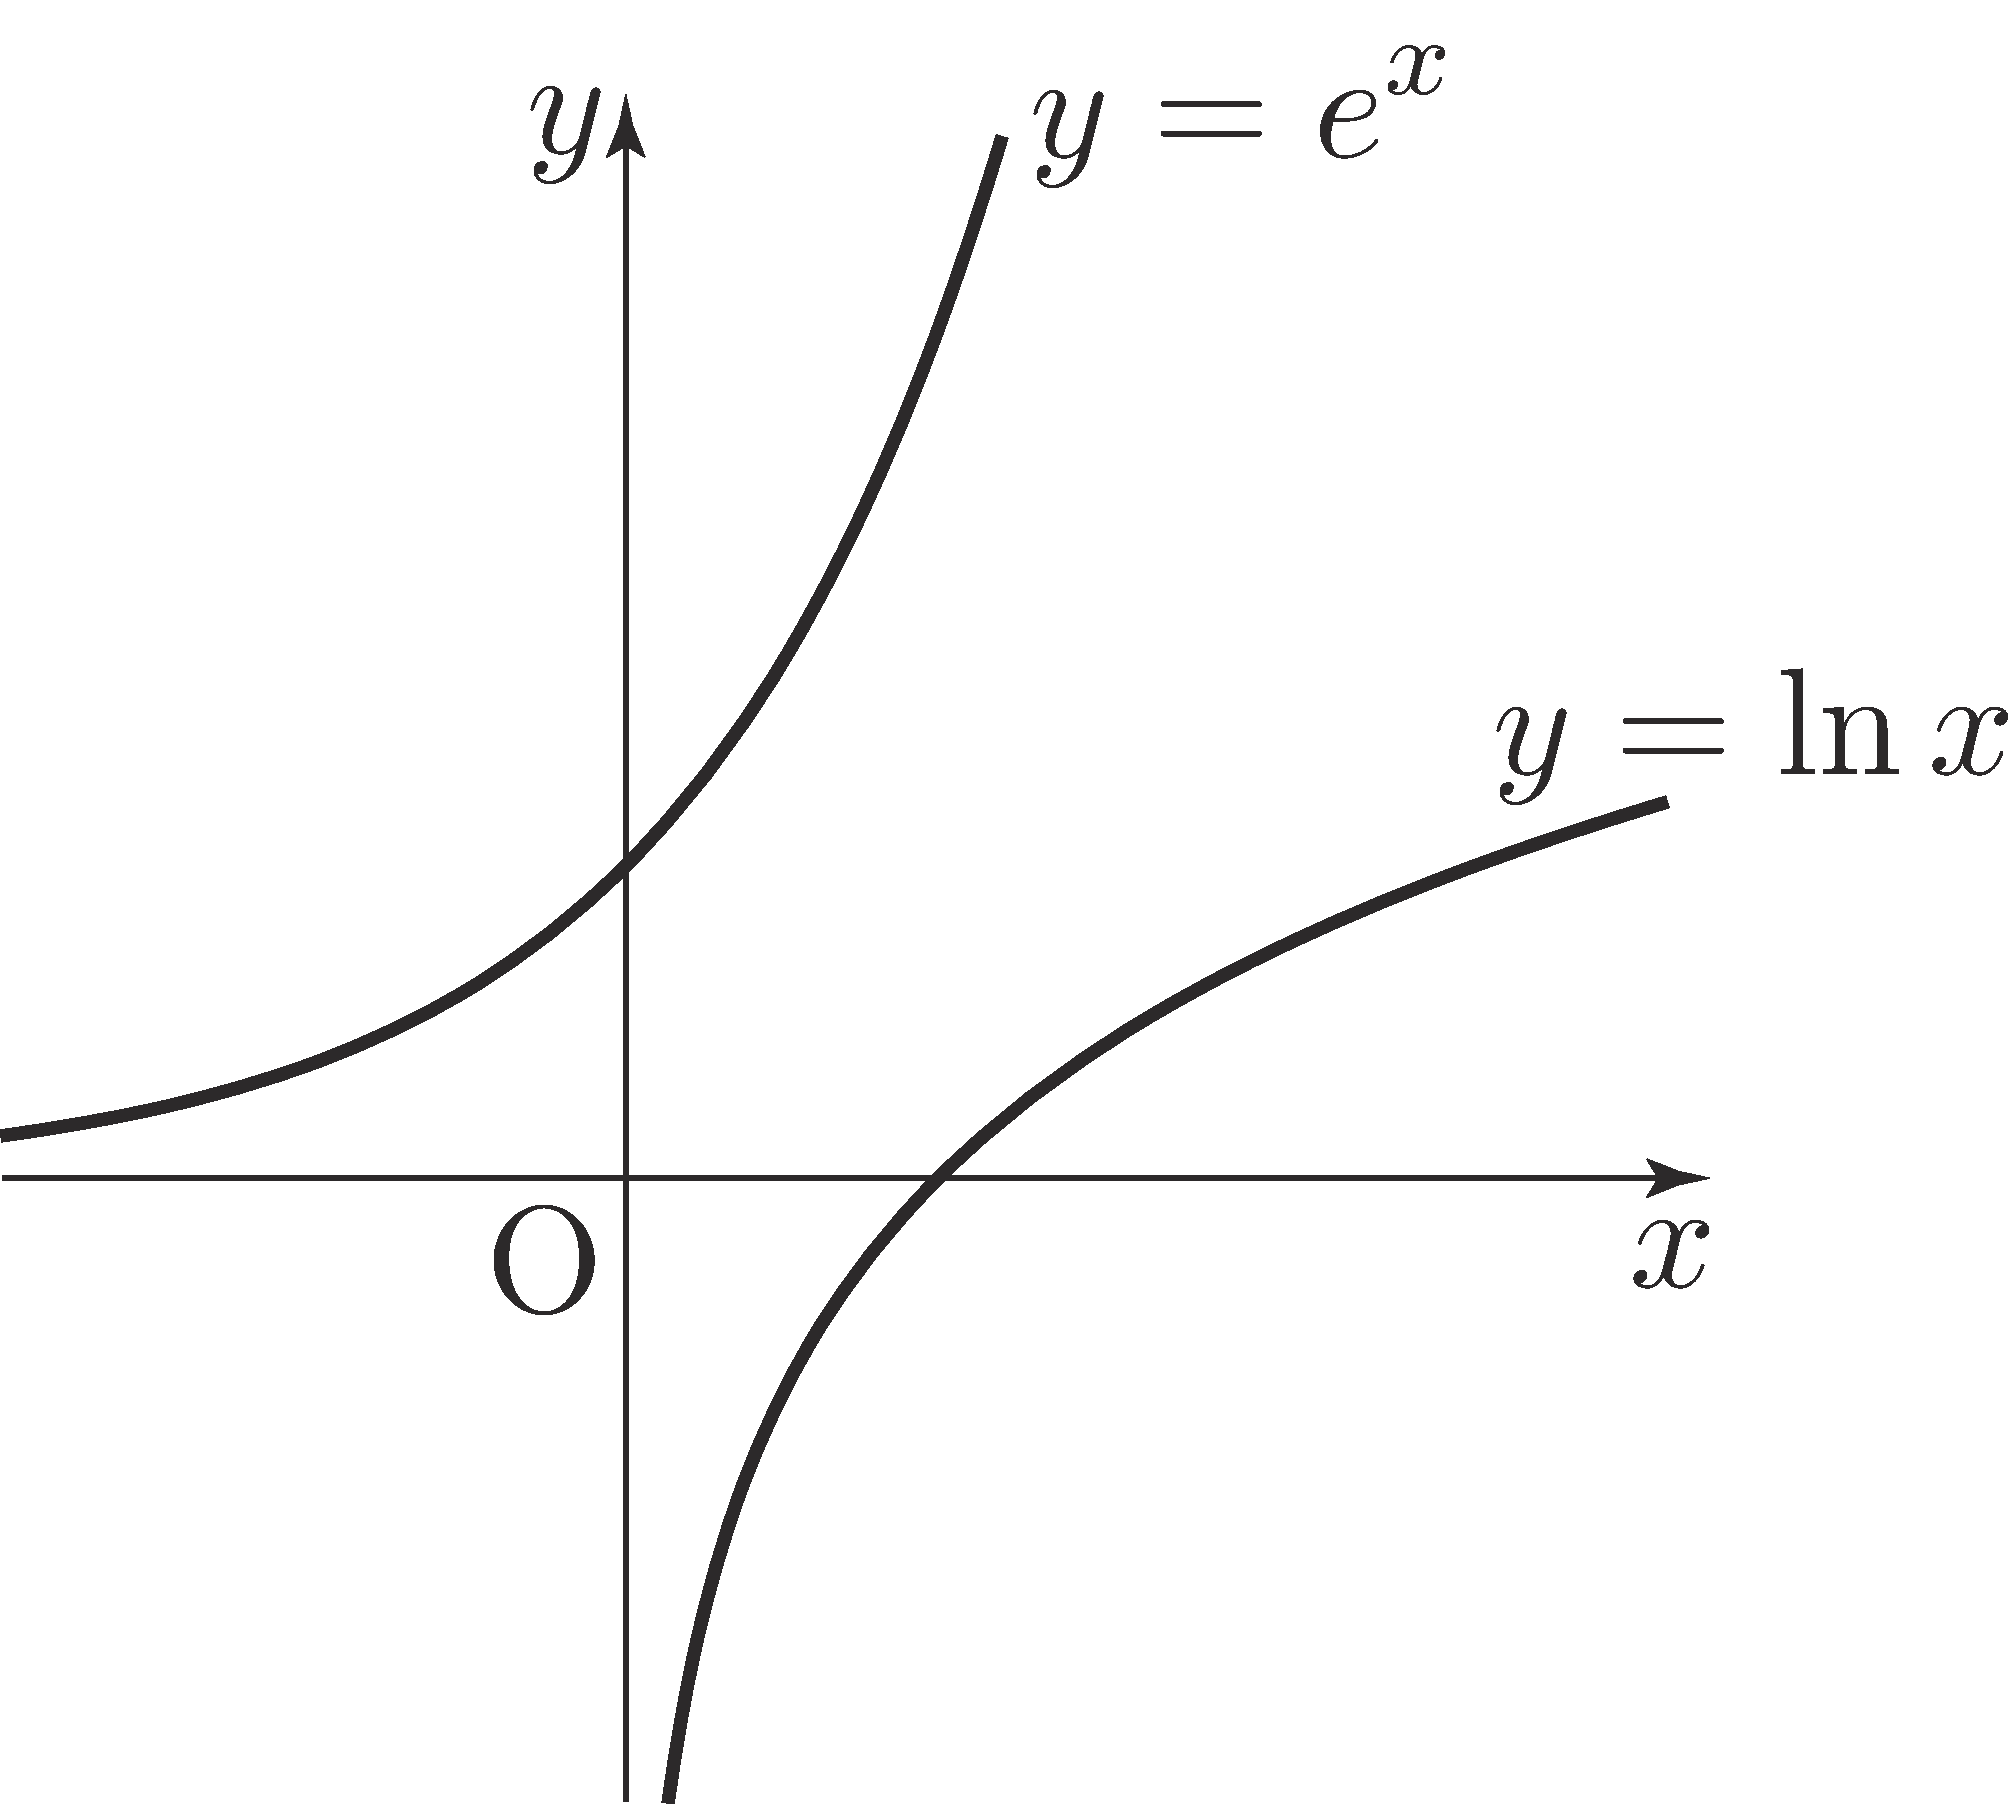
\includegraphics[scale=\pgfkeysvalueof{picsize}]{DBs/pic/zery_09.pdf}\
	\end{center}앞서 Graph 0.1)에서 설명했듯, 함수의 정의역은 좌표평면에서 그래프가 그려지는 가로 범위를 결정합니다. 이는 논의 대상이 되는 $x$의 값의 범위를 결정하므로 매우 중요합니다. 예를 들어 $y=\ln x$는 양수 $x$에 대해서만 다루지만, $y=e^x$는 모든 실수 $x$에 대해서 다룹니다.

\section{치역}
\begin{center} 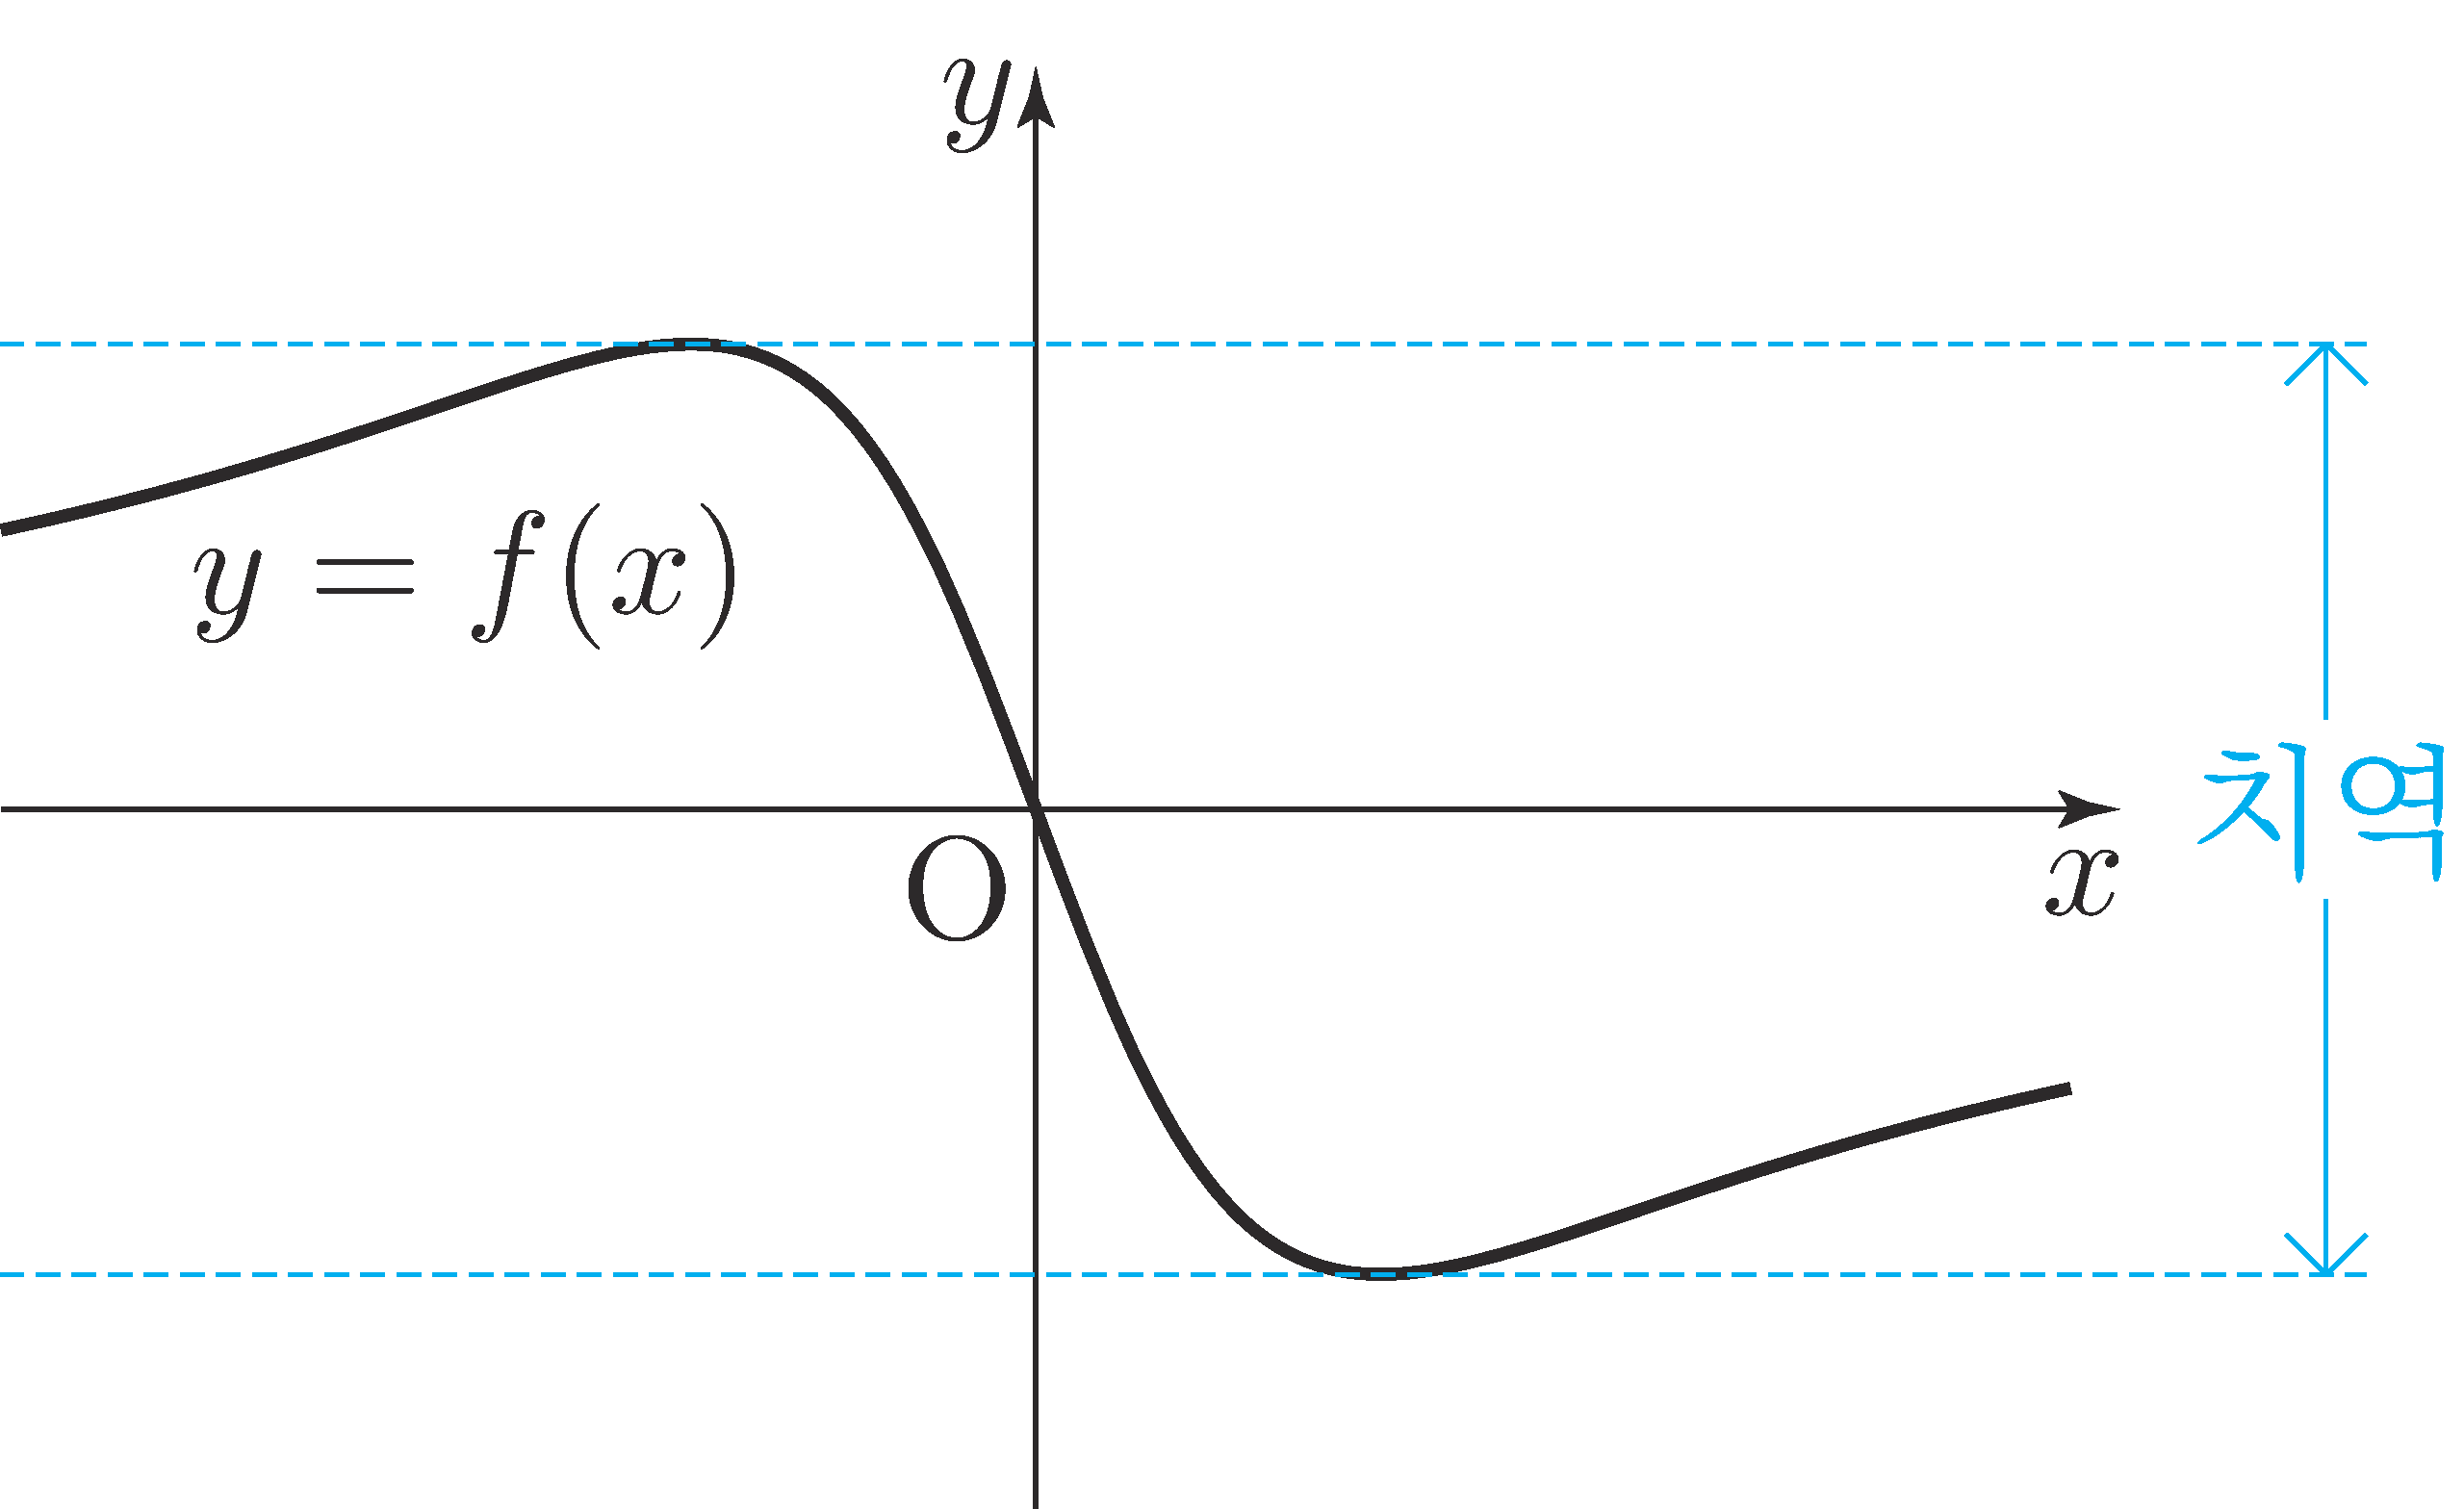
\includegraphics[scale=\pgfkeysvalueof{picsize}]{DBs/pic/zery_10.pdf}\
	\end{center}함수의 치역은 좌표평면에서 그래프가 그려지는 세로구간이 어떤지를 결정합니다. 이는 이후에 배울 최점, 쵯값과 매우 밀접한 연관을 가지므로 매우 중요합니다. 

\section{좌표축과의 교점(절편)}
\begin{center} 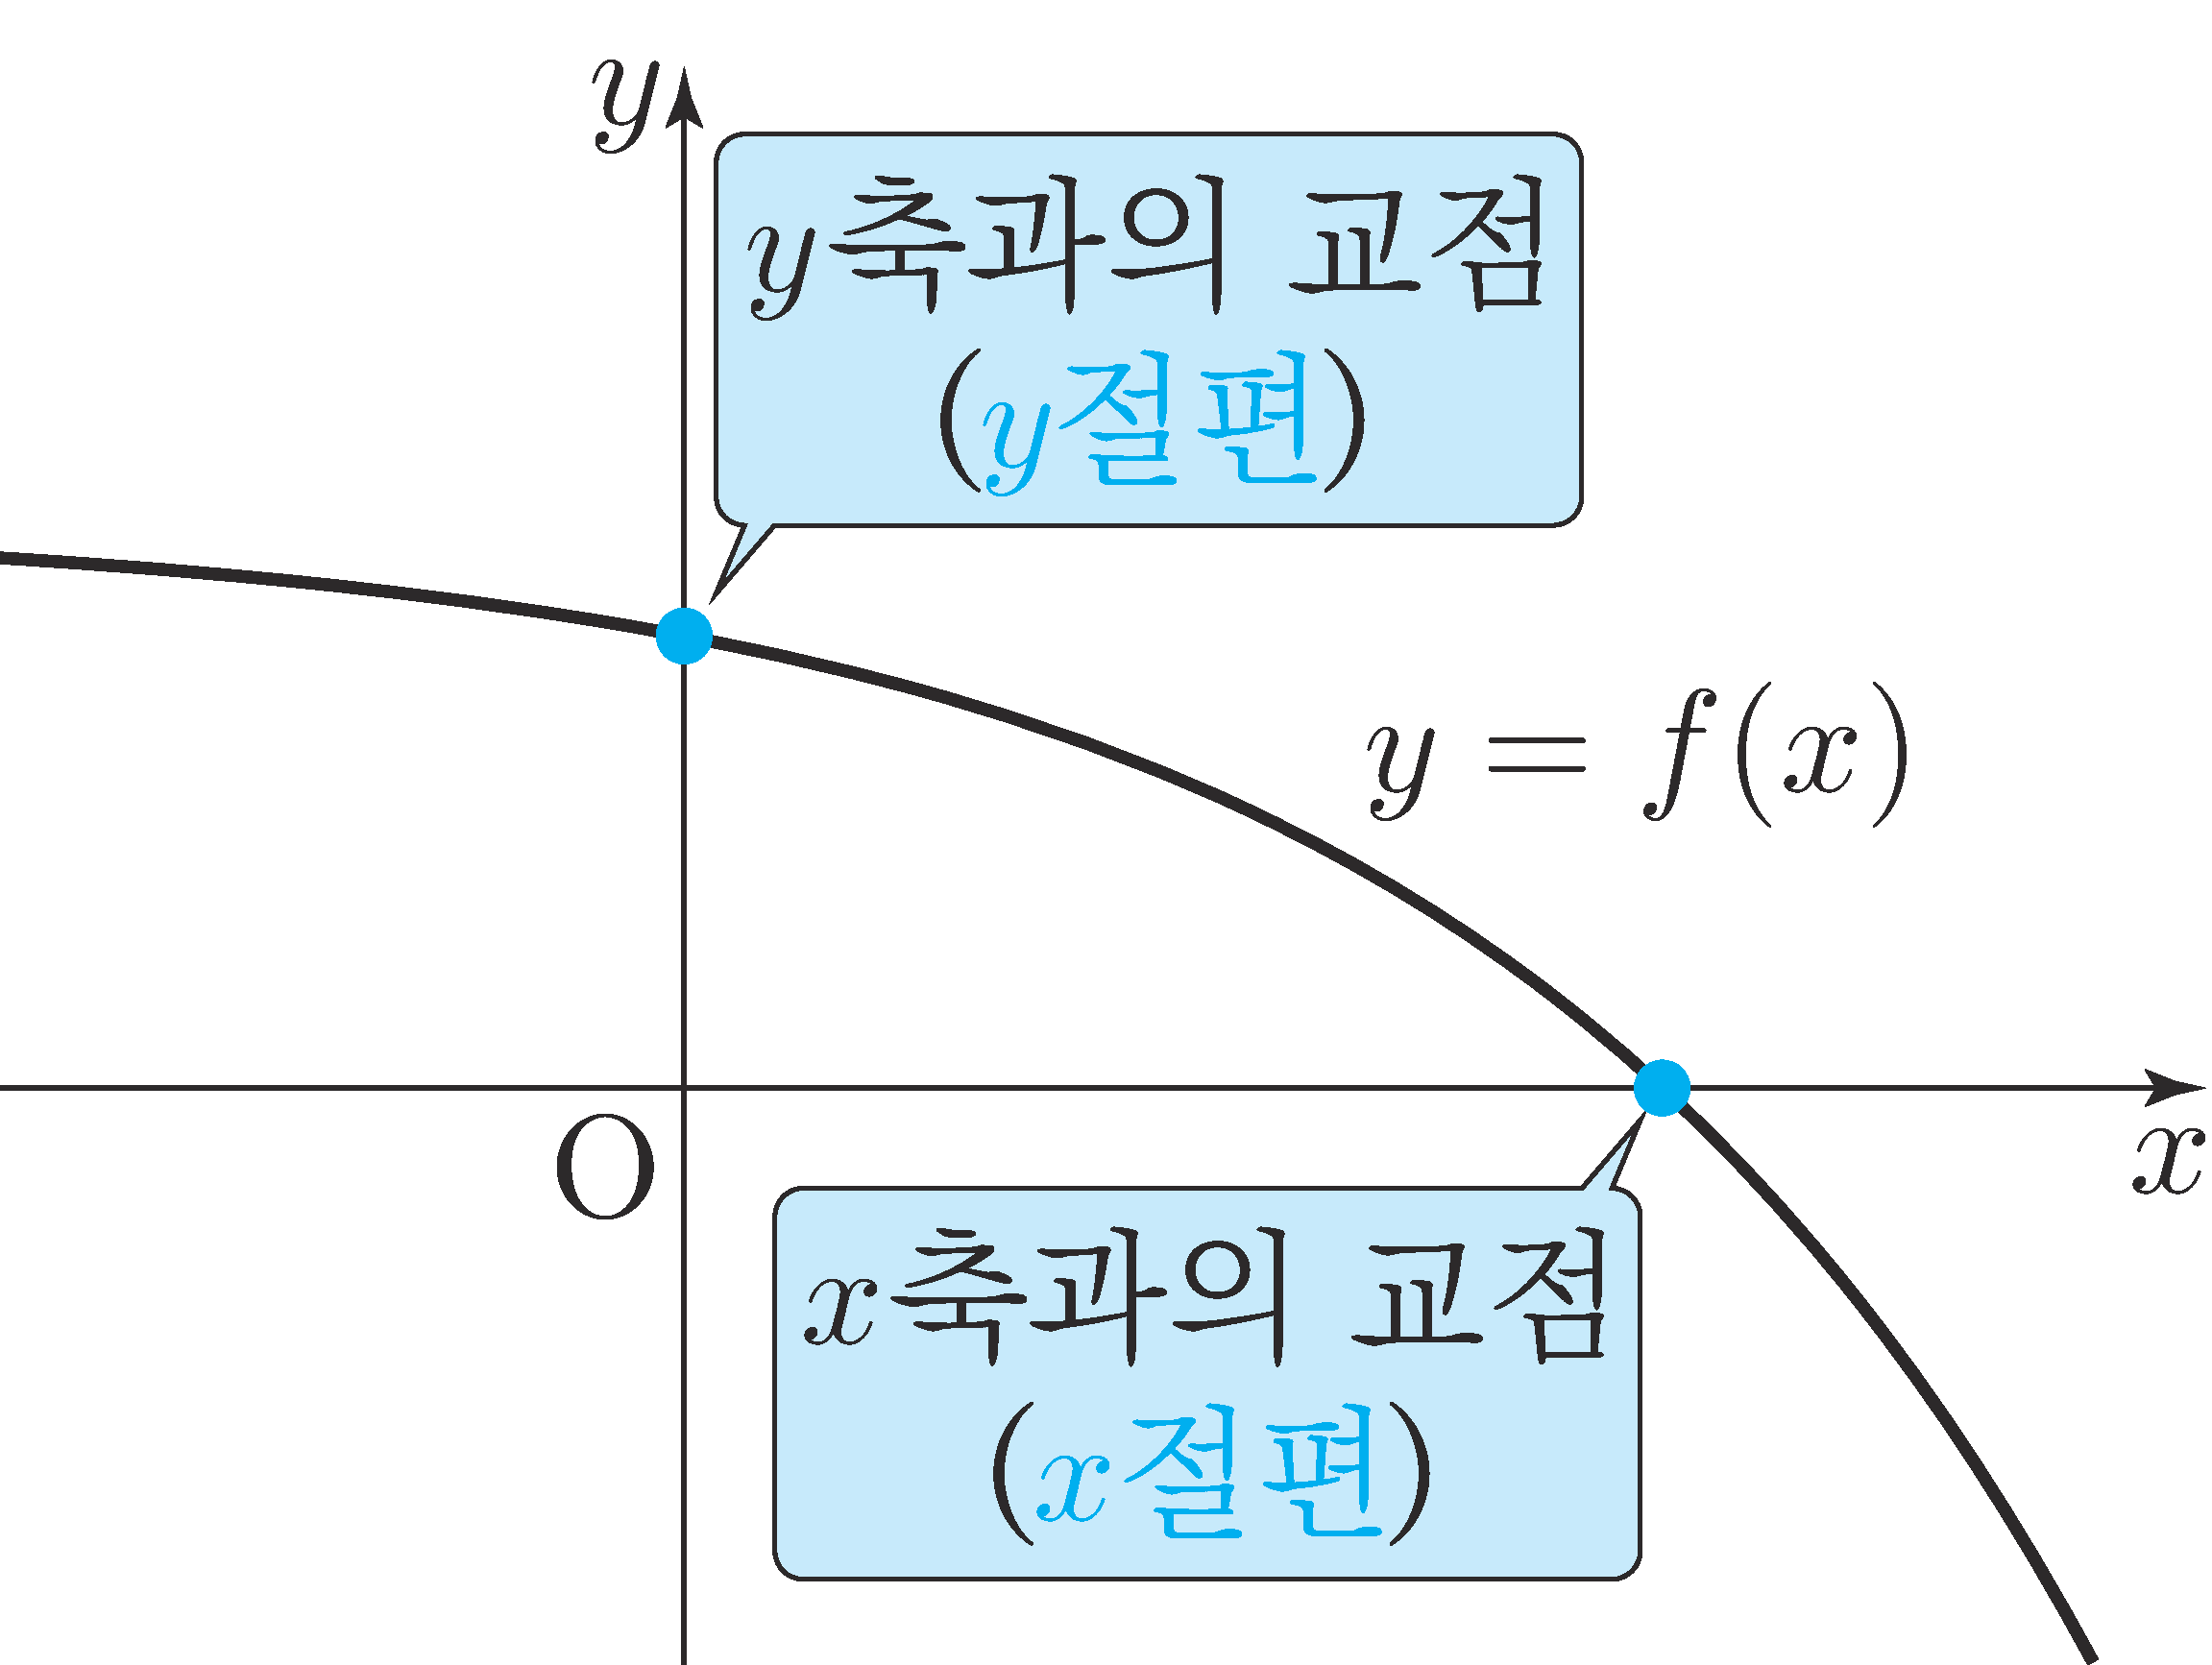
\includegraphics[scale=\pgfkeysvalueof{picsize}]{DBs/pic/zery_11.pdf}\
	\end{center}$x$축과 $y$축은 좌표평면을 네 개의 사분면으로 구분하는 기준이 됩니다. 따라서 각 축과의 교점은 그래프의 위치에 대한 개략적인 정보를 준다는 점에서 중요합니다.\mn[-5\blskip]{그만큼 자주 쓰이는 대상이므로, 매번 `축과의 교점'이라 부르는 것보다는 간결한 이름을 지어주는 것이 편리할 것입니다. 따라서 직선에서만 쓰이는 용어인 `절편'을 함수의 그래프에도 적용하여 함수의 그래프와 $x$축과의 교점의 $x$좌표를 \iterm{$x$절편}{}, \mbox{$y$축과의} 교점의 $y$좌표를 \iterm{$y$절편}{}이라 부르기로 합시다.}{}
\clearpage\begin{center} 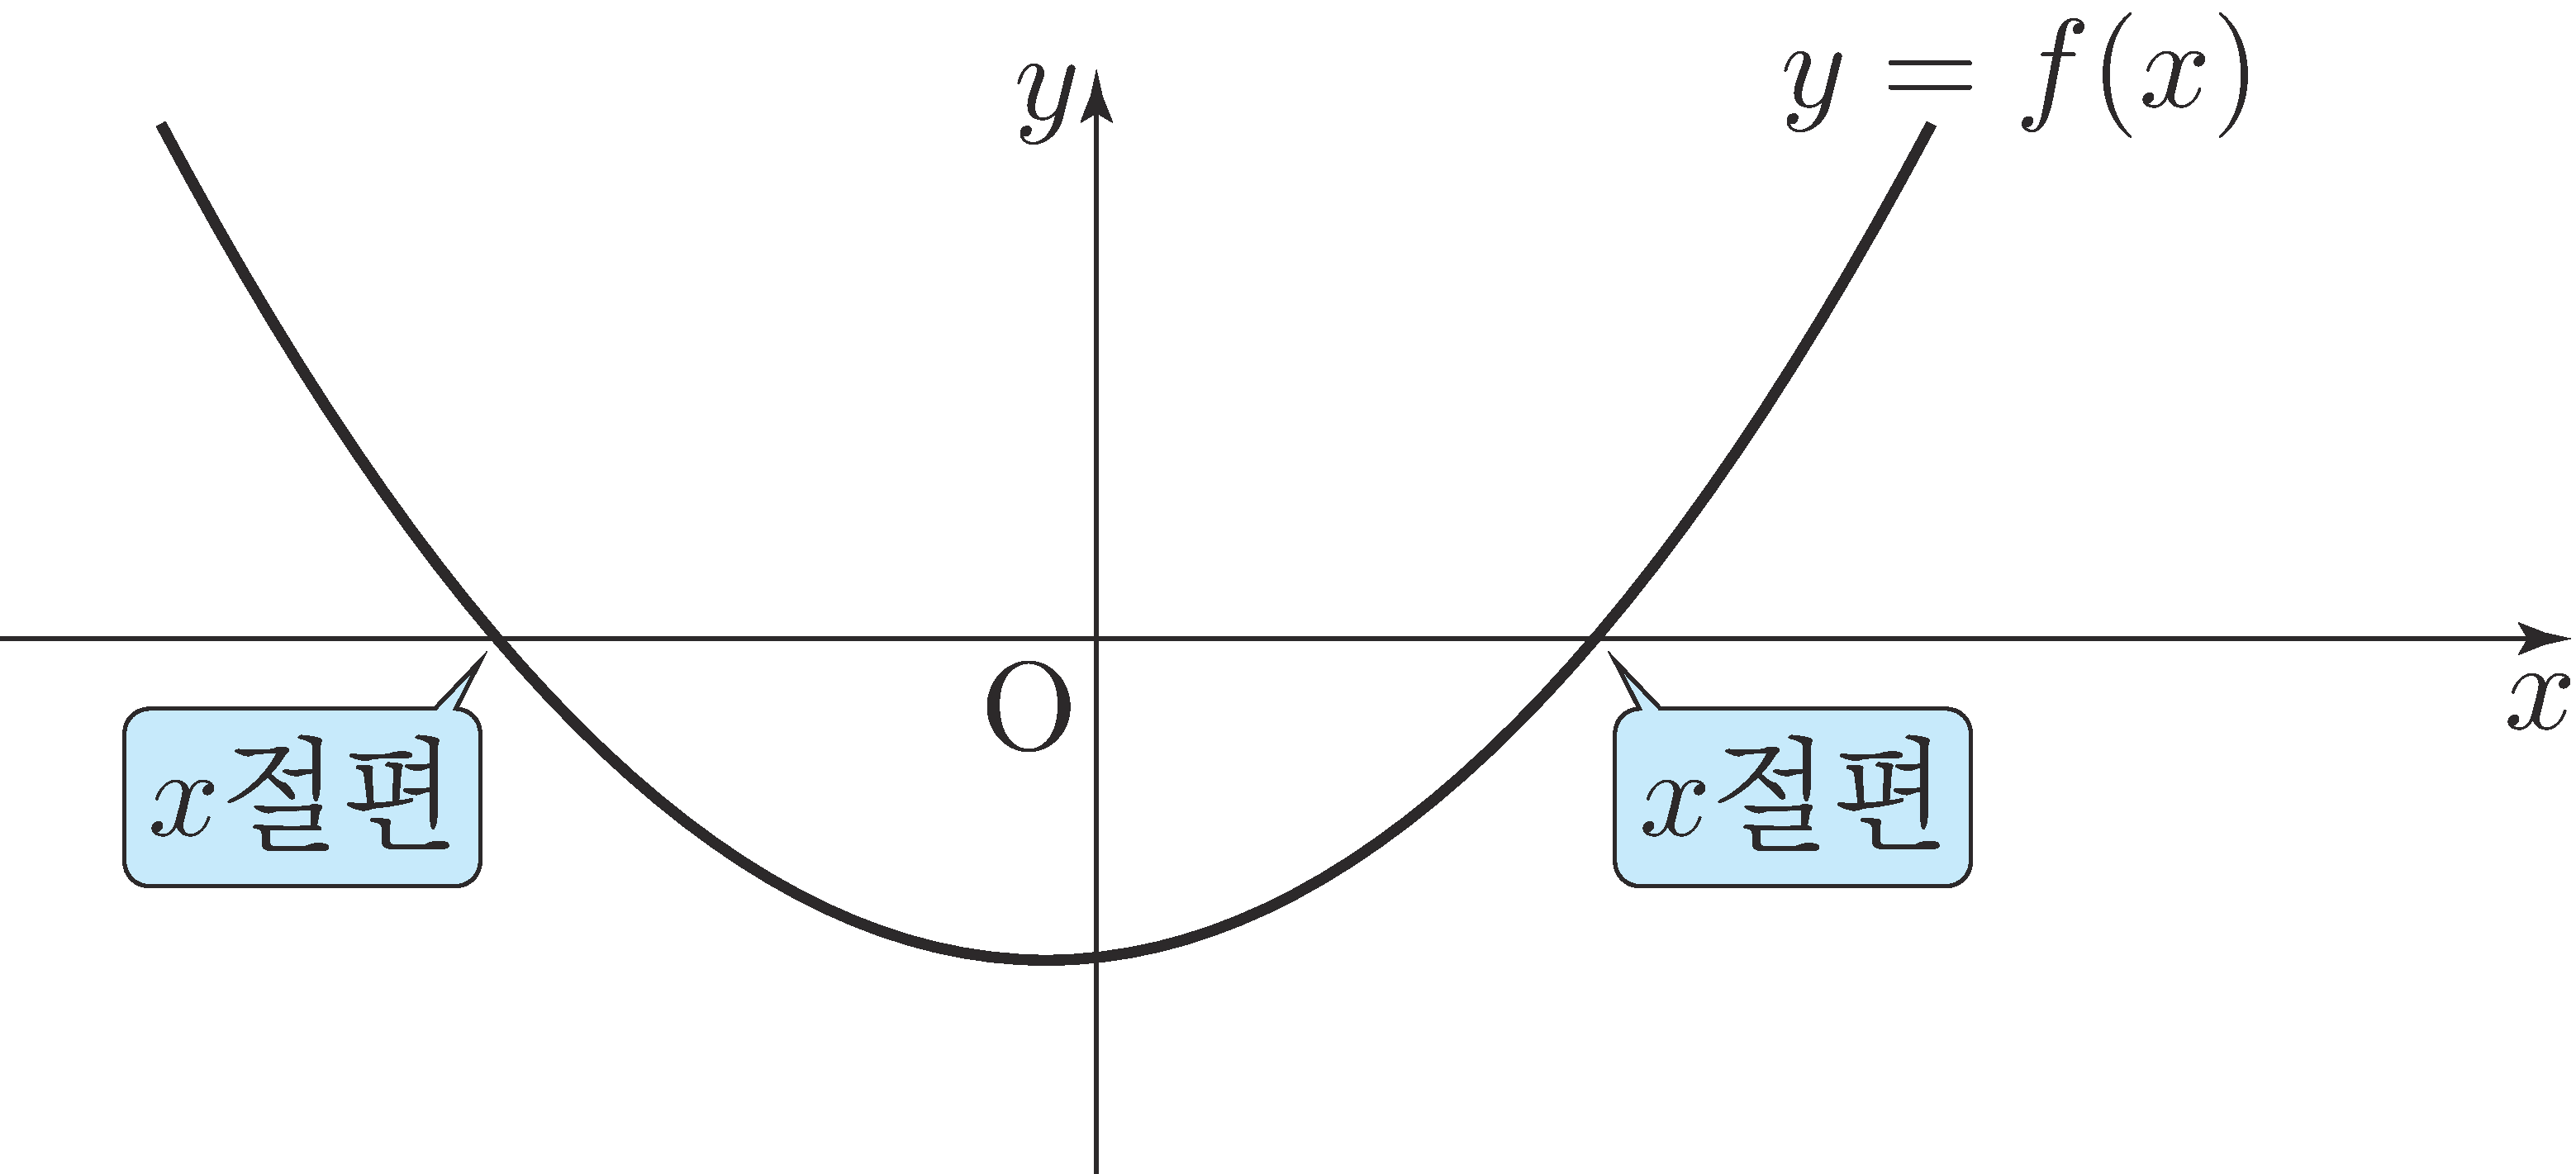
\includegraphics[scale=\pgfkeysvalueof{picsize}]{DBs/pic/zery_12.pdf}\
	\end{center}$x$절편은 방정식 $f\left( x \right) = 0$의 해라는 점에서도 중요하고, 연속함수인 경우 함숫값 부호 변화의 가능성을 따지는 기준점이 되므로 매우 중요합니다. 한 곡선 $y=f\left( x \right) $에 대하여 $x$절편은 존재하지 않을 수도 있고, 오직 하나만 존재할 수도 있고, 여러 개 존재할 수도 있습니다.
\begin{center} 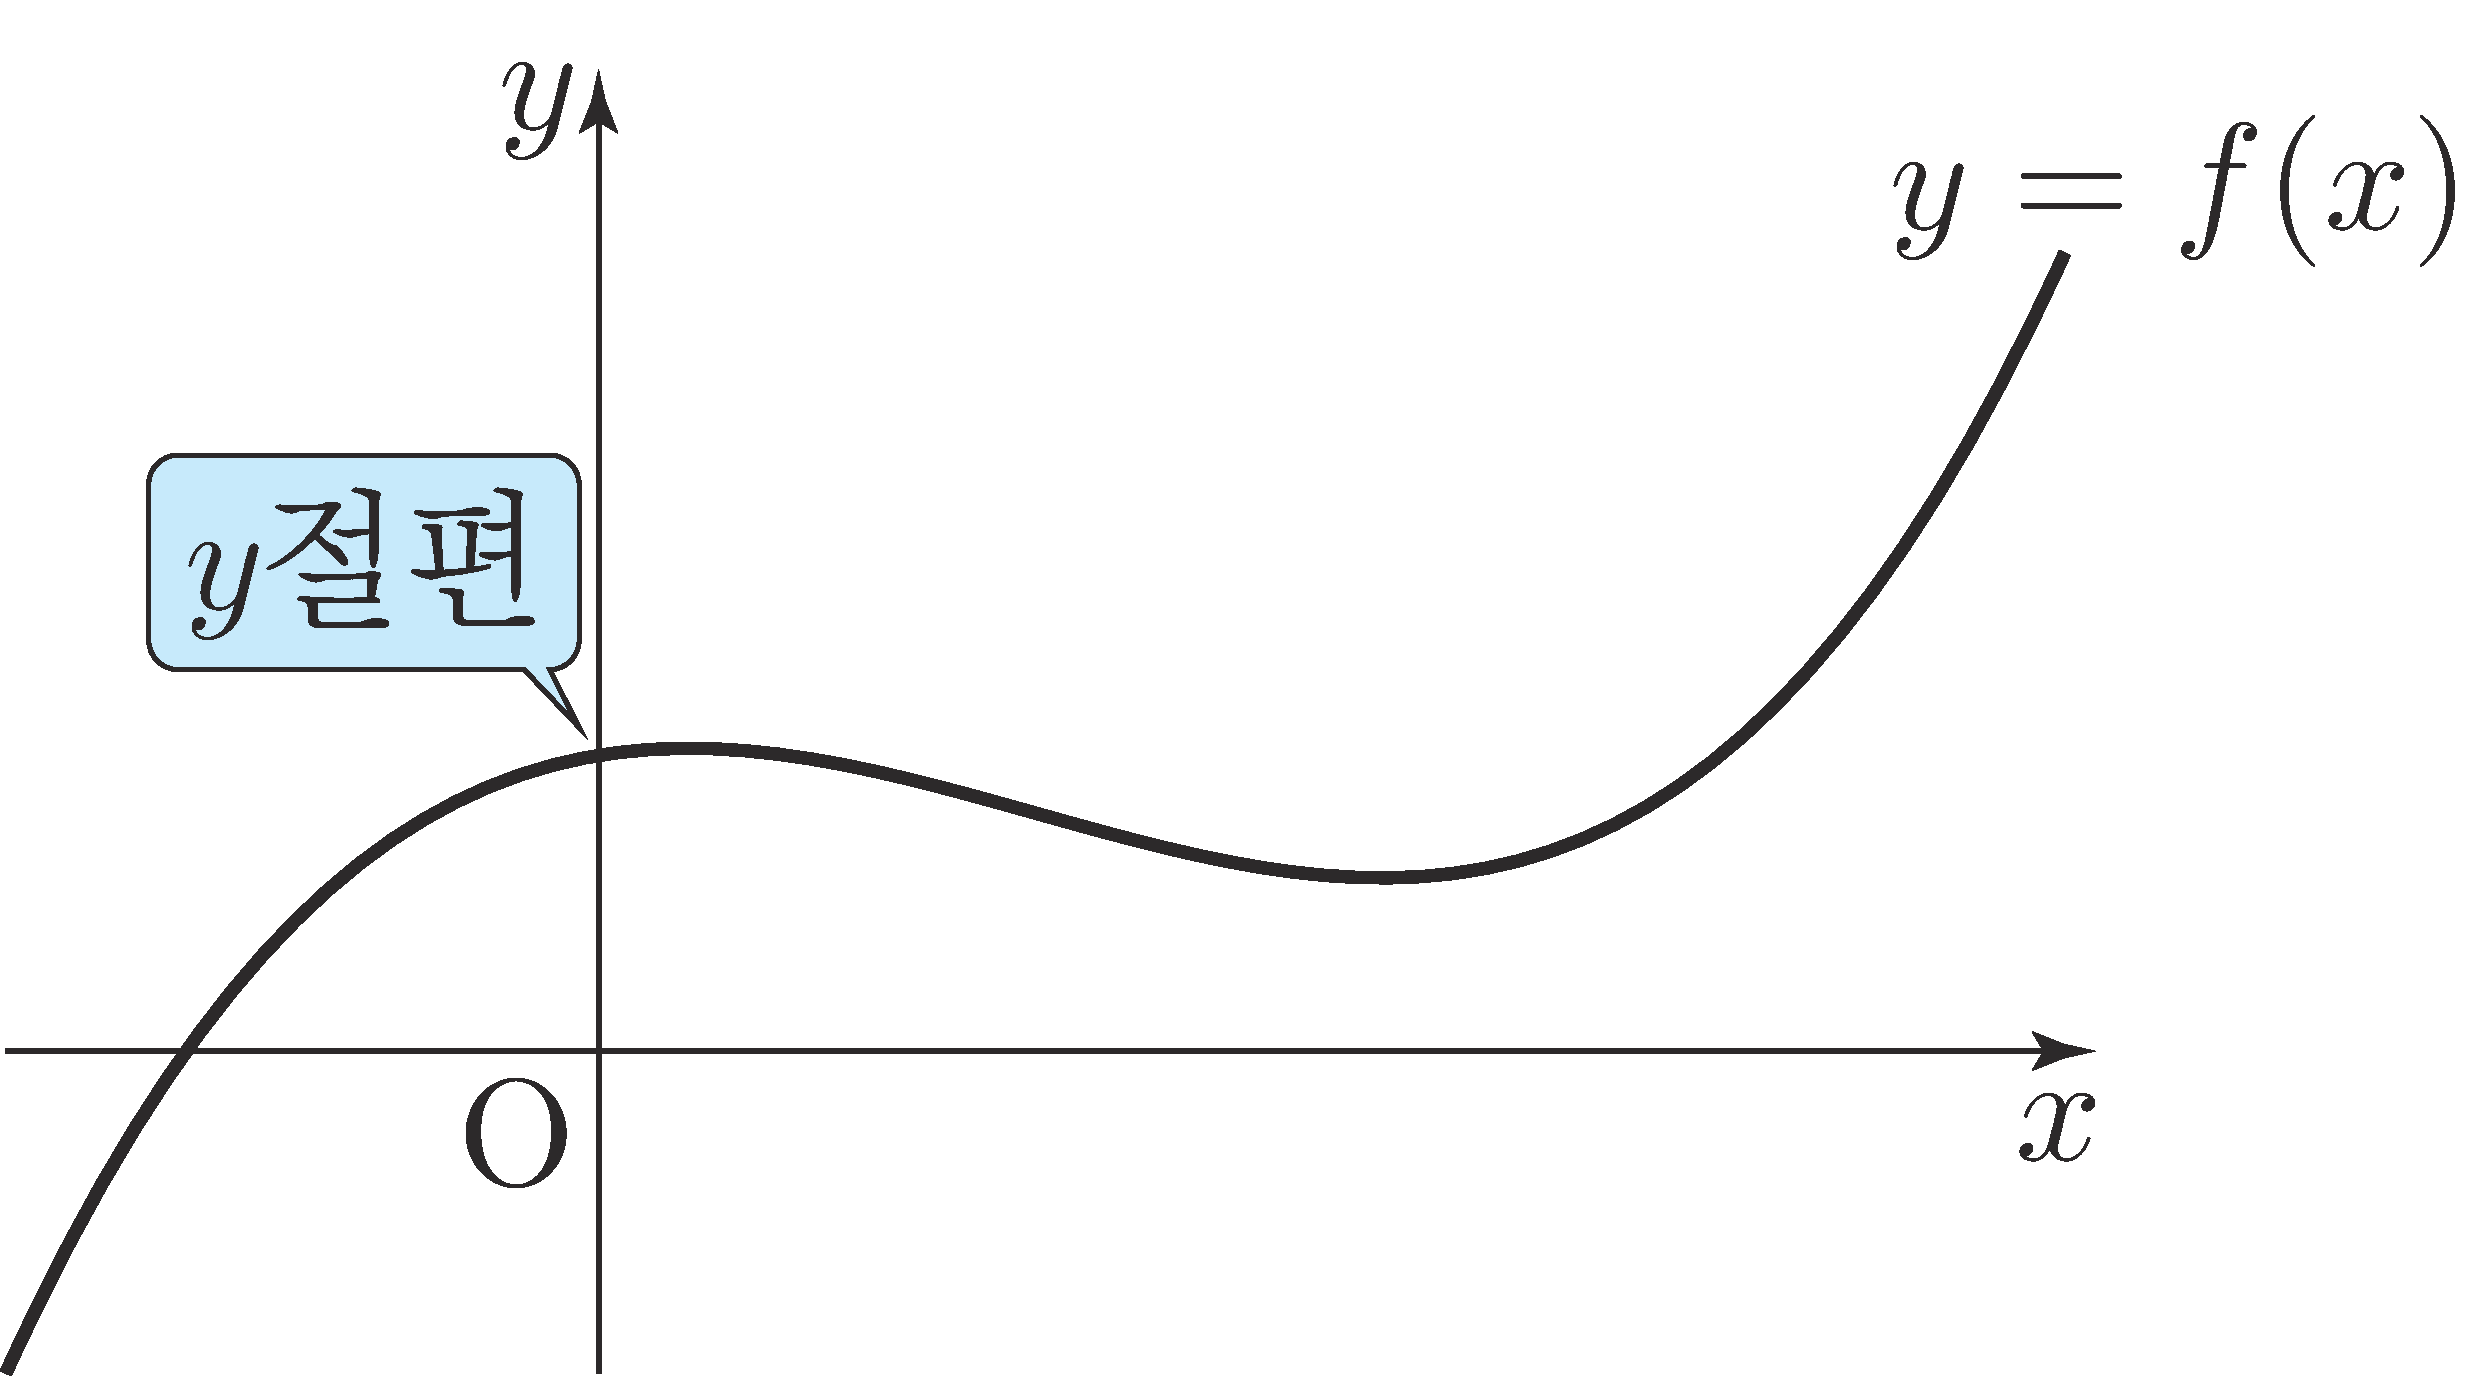
\includegraphics[scale=\pgfkeysvalueof{picsize}]{DBs/pic/zery_13.pdf}\
	\end{center}다항함수의 경우 주어진 식에서 바로 $y$축과의 교점을 알아낼 수 있는 경우가 많아 자주 쓰이는 점 중 하나입니다. $y$절편은, 반드시 유일하다는 점에서\mn{$0$이 정의역에 포함되지 않은 경우에는 존재하지 않습니다.}{} 특별한 의미를 갖습니다. 

\section{함숫값의 부호}
\begin{center} 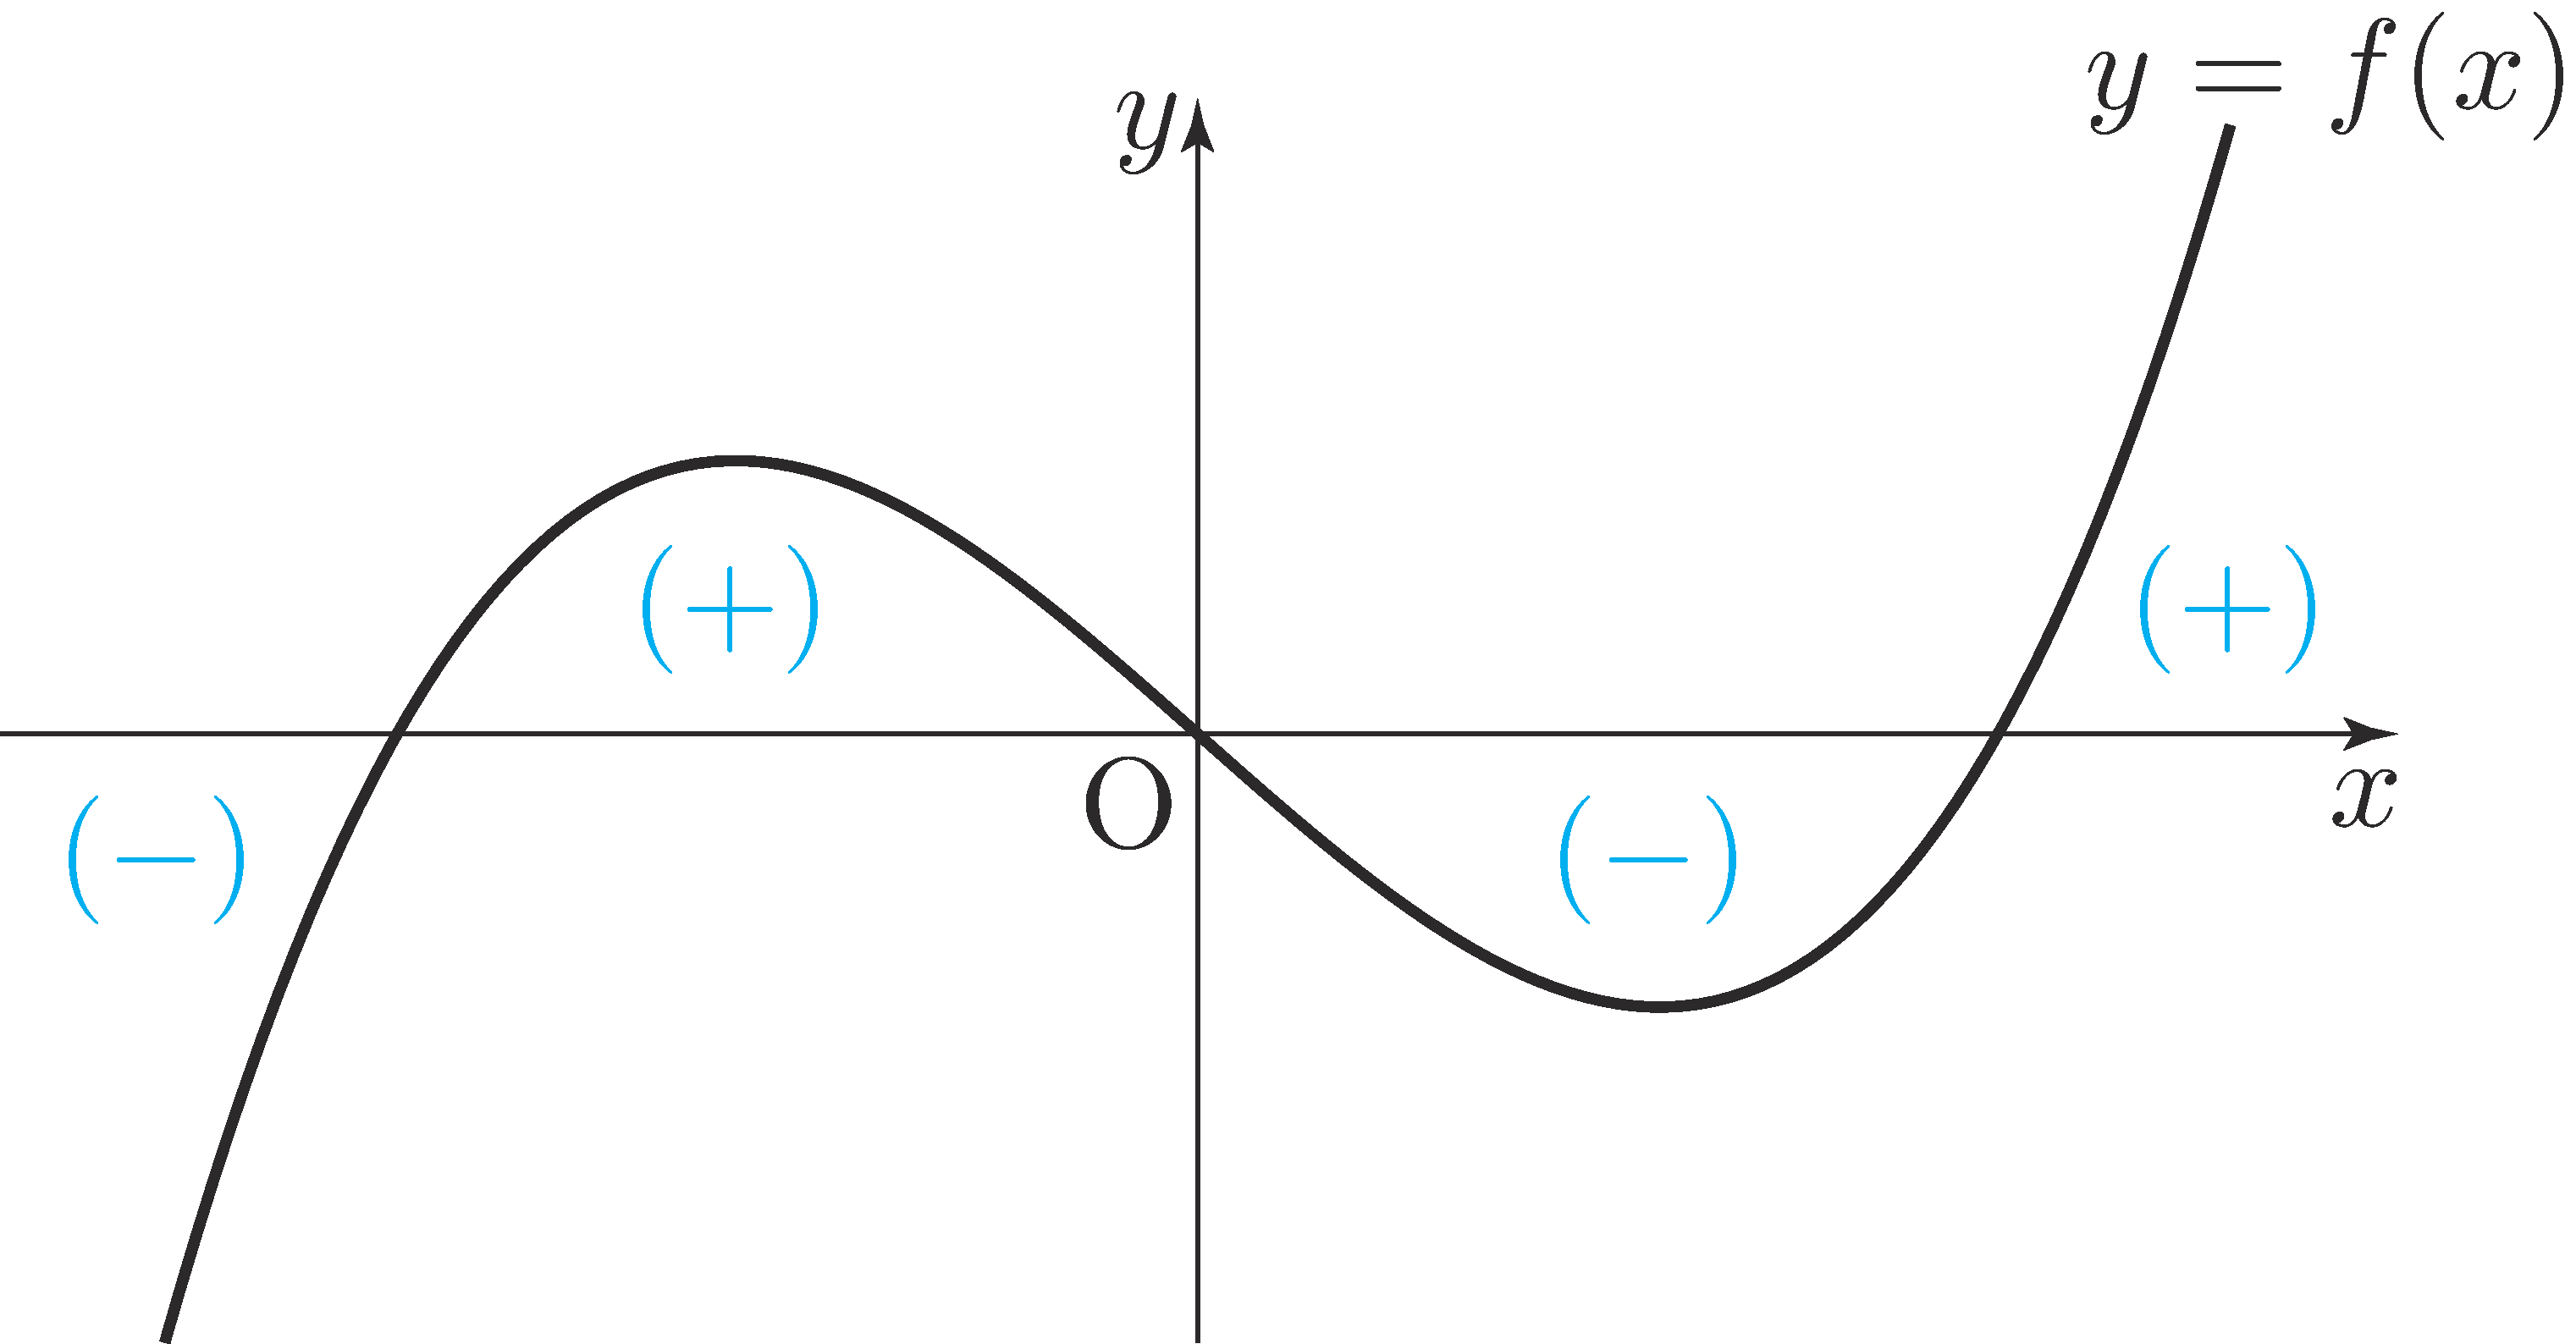
\includegraphics[scale=\pgfkeysvalueof{picsize}]{DBs/pic/zery_14.pdf}\
	\end{center}$x$좌표와 $y$좌표가 모두 실수이므로, 실수를 바라보는 관점에 의하면 부호를 기준으로 생각하는 것은 자연스럽습니다. 이때 $x$좌표는 이미 좌표평면에 의해 부호를 기준으로 나뉘어 있으므로, $y$좌표인 $f\left( x \right) $의 부호가 중요합니다. 또한 $f\left( x \right) $의 부호가 어떤지에 따라 $x$의 범위를 생각할 수 있습니다. 그러므로 각각의 범위 또한 중요합니다.
\clearpage
\section{한 점 $\xy{a}{f\left( a \right) }$가 주어졌을 때  좌표평면에서 뽑아낼 수 있는 정보}
\begin{center} 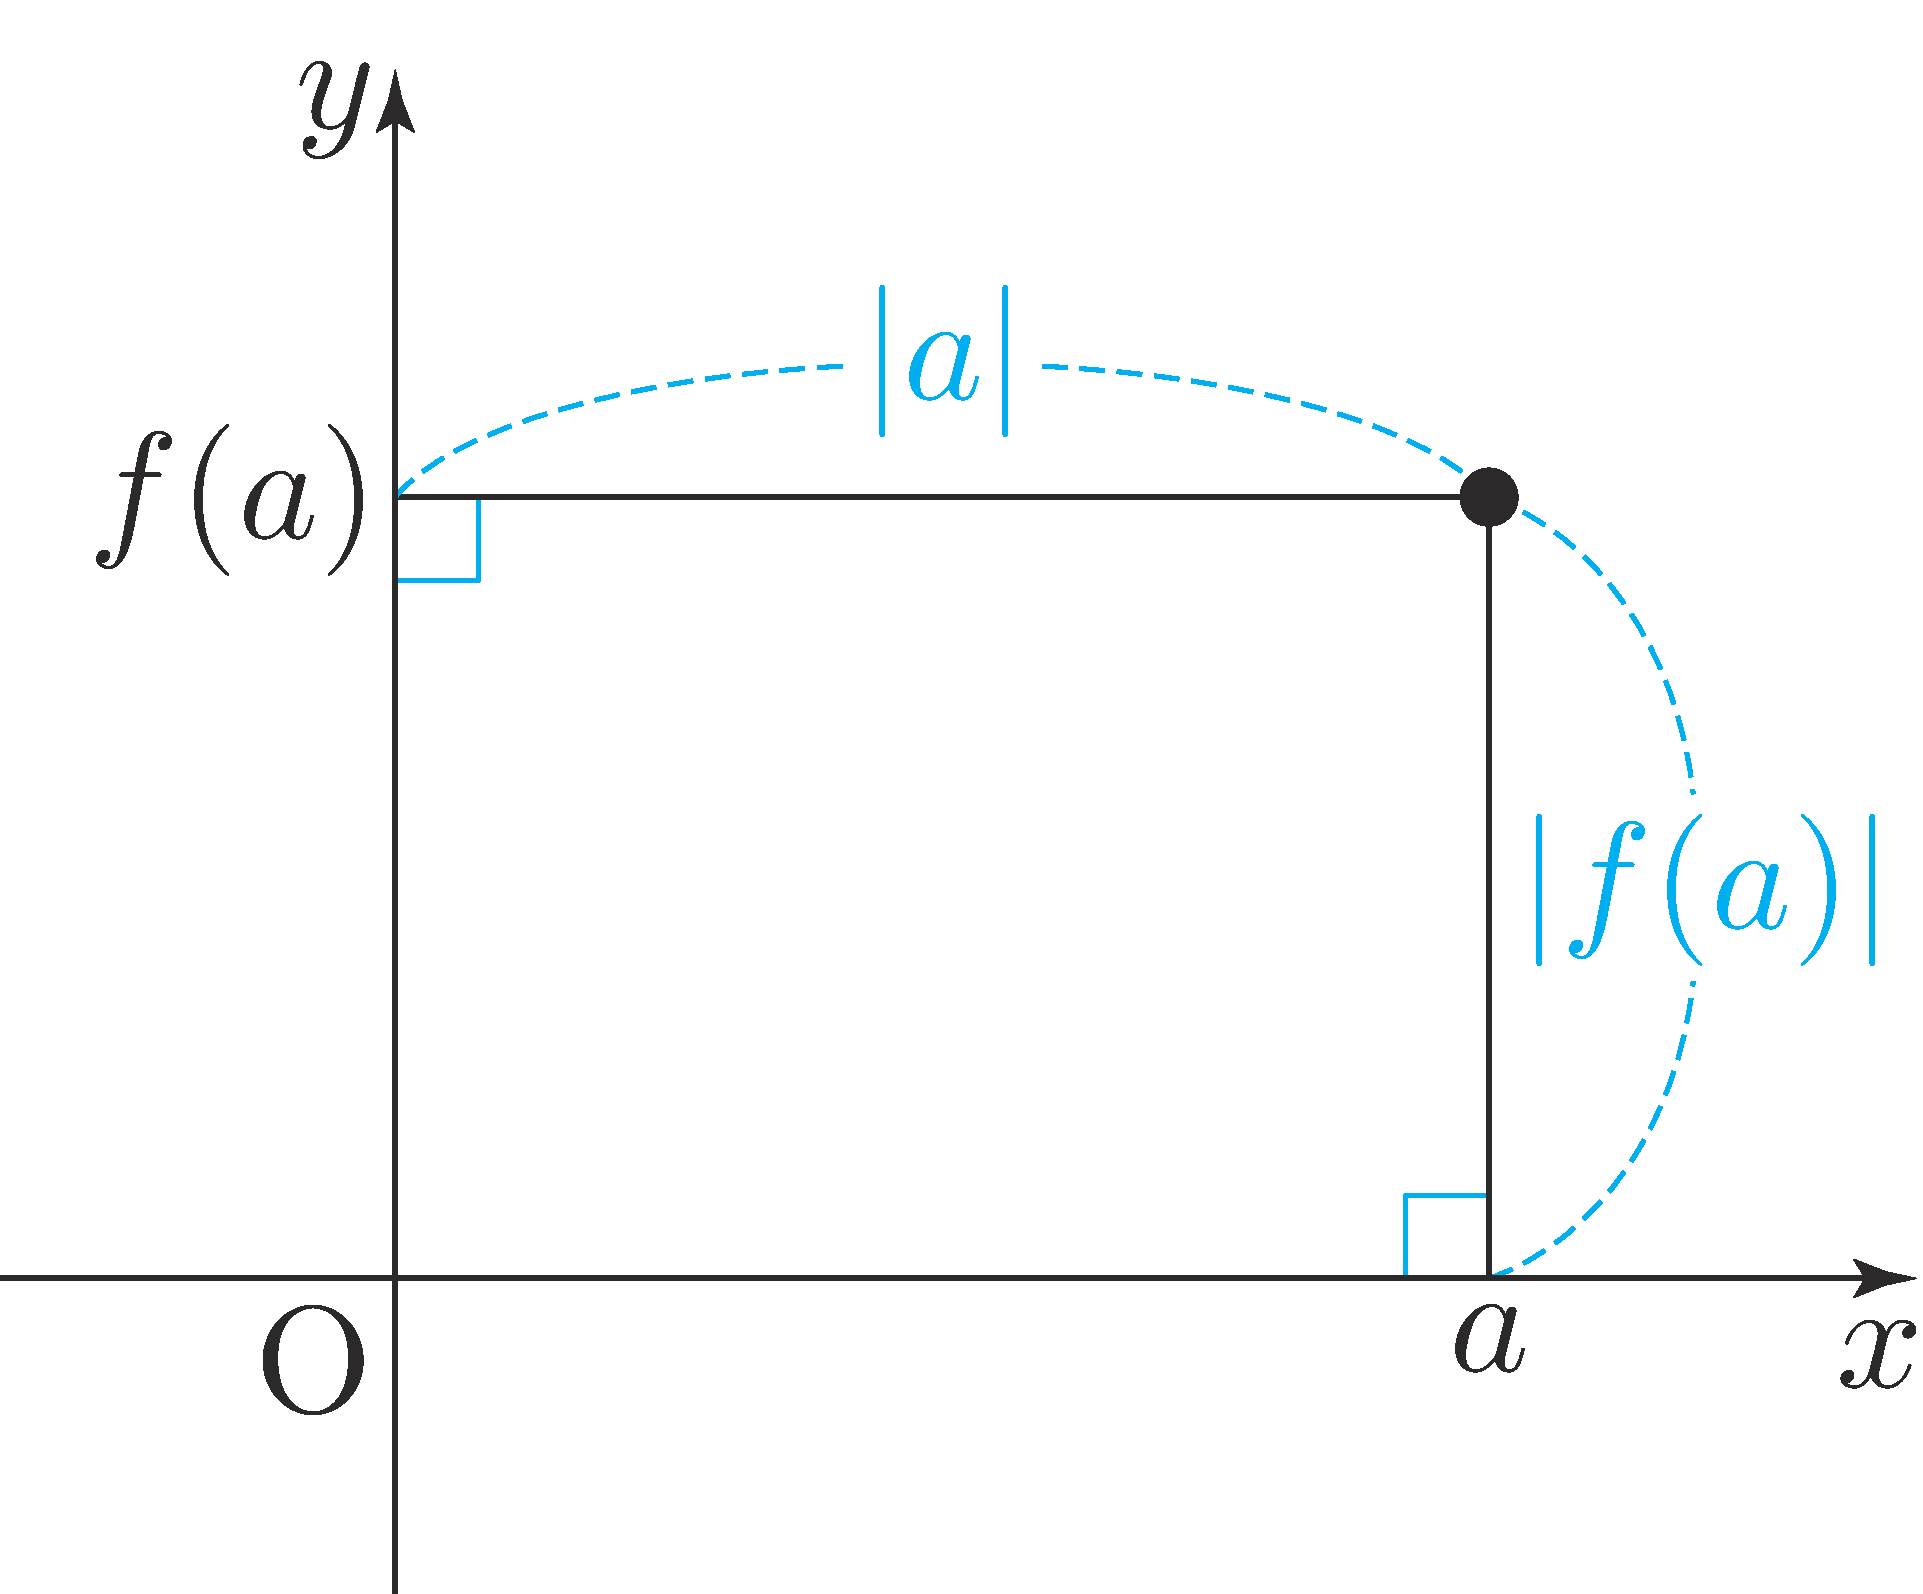
\includegraphics[scale=\pgfkeysvalueof{picsize}]{DBs/pic/zery_15.pdf}\
	\end{center}한 점 $\xy{a}{f\left( a \right) }$ $(a \ne 0)$가 주어졌다고 해봅시다. 이 점에서 각 좌표축에 수선의 발을 내리는 것은 자연스럽습니다. 이때 $x$축까지의 거리는 $\abs{f\left( a \right) }$, $y$축까지의 거리는 $\abs{a}$입니다.
\begin{center} 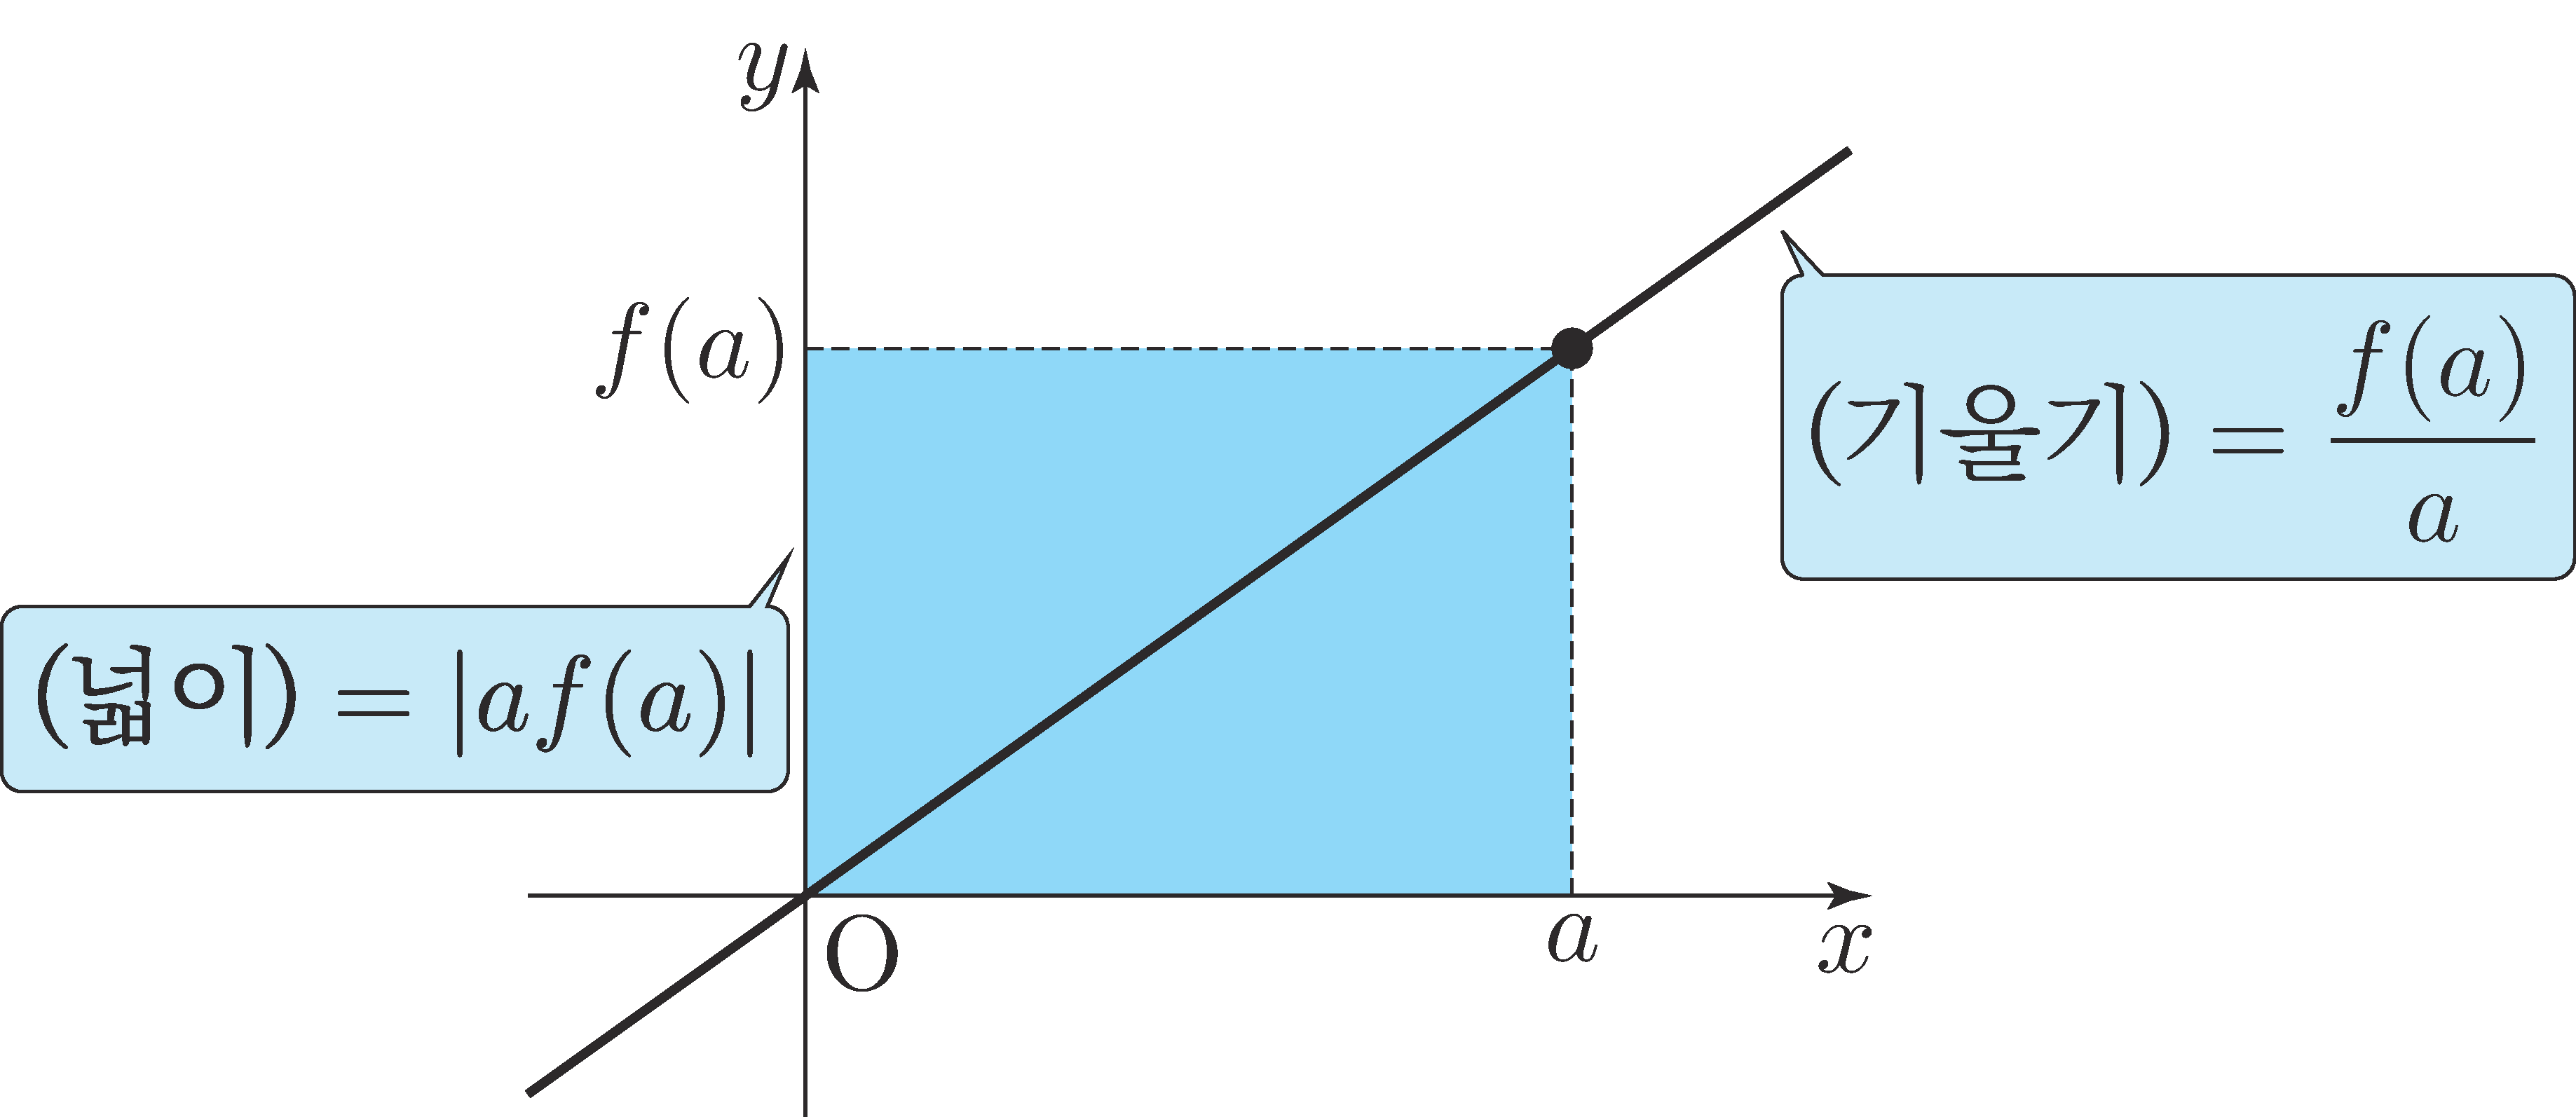
\includegraphics[scale=\pgfkeysvalueof{picsize}]{DBs/pic/zery_16.pdf}\
	\end{center}한편 기하학적인 관점에서 이 점의 $x$좌표와 $y$좌표를 활용할 수 있습니다. 좌표평면에 기본적으로 주어진 점인 원점과 이 점을 지나는 직선을 생각한다면 그 직선의 기울기는 $\dfrac{f\left( a \right) }{a}$입니다. 또한 원점과 이 점을 한 대각선으로 하는 직사각형을 생각할 수 있으며, 이 직사각형의 넓이는 $\abs{af\left( a \right) }$입니다. 원점이 아니라 다른 점이 주어졌다면, 그 점을 이용해서 기울기와 넓이를 생각할 수도 있습니다.
%\clearpage
\begin{center} 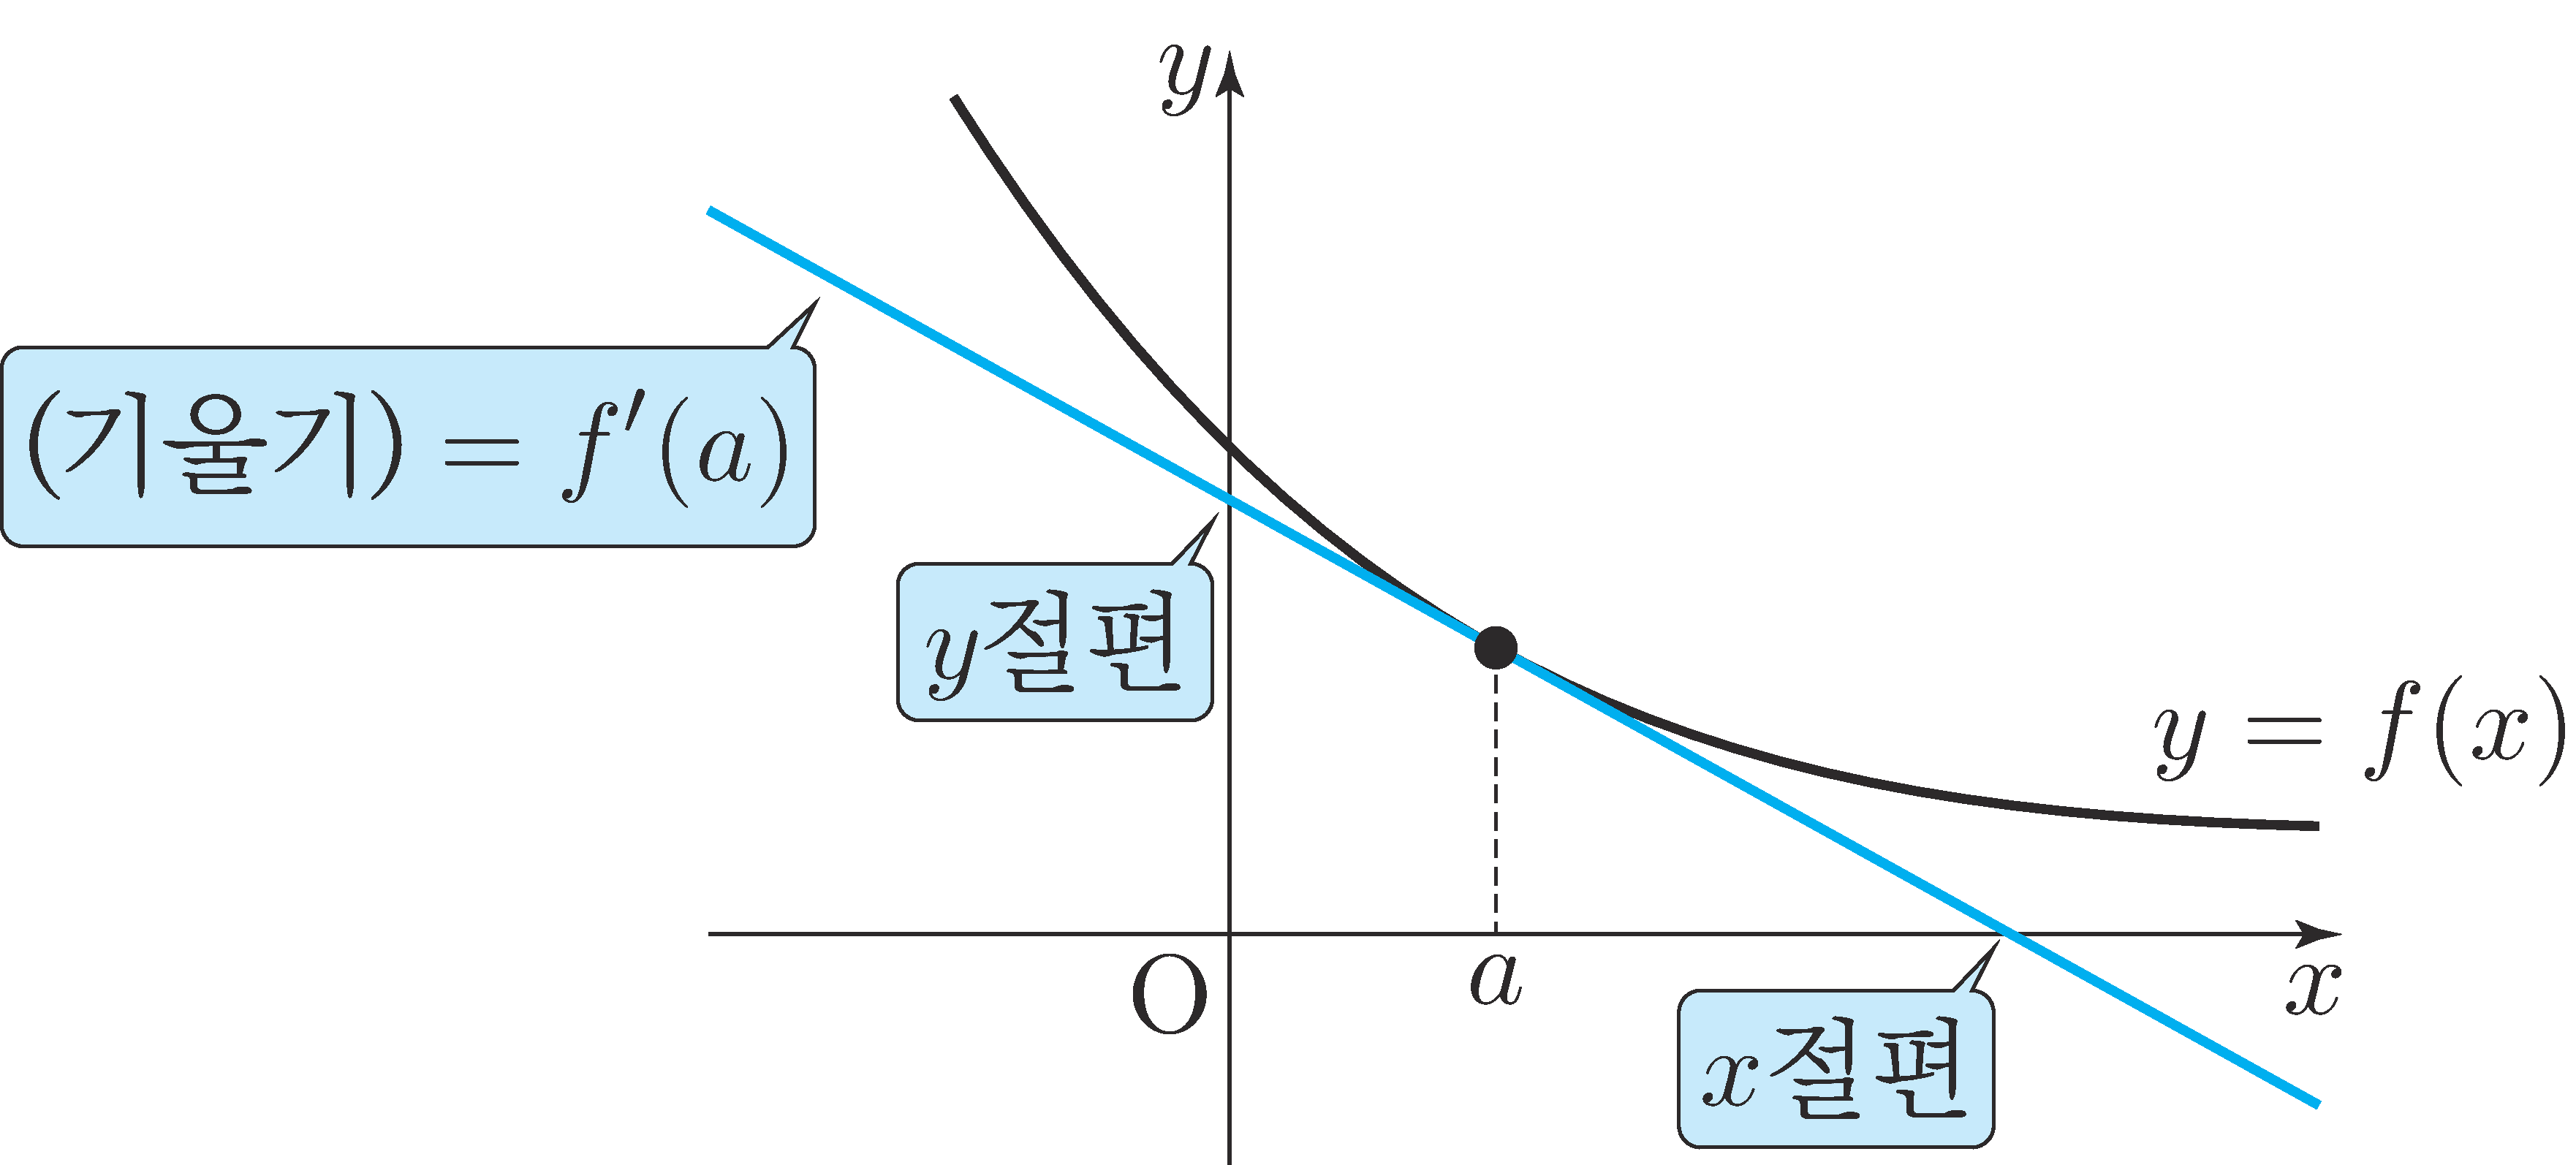
\includegraphics[scale=\pgfkeysvalueof{picsize}]{DBs/pic/zery_17.pdf}\
	\end{center}만약 함수 $f\left( x \right) $가 미분가능하다면 접선의 기울기인 $f'\left( a \right) $를 생각할 수 있고, 접선의 $x$절편과 $y$절편 또한 생각할 수 있습니다.



\mychapter{그래프로 해석하는 방정식과 부등식}{}

\section{방정식과 그래프}
\begin{center} 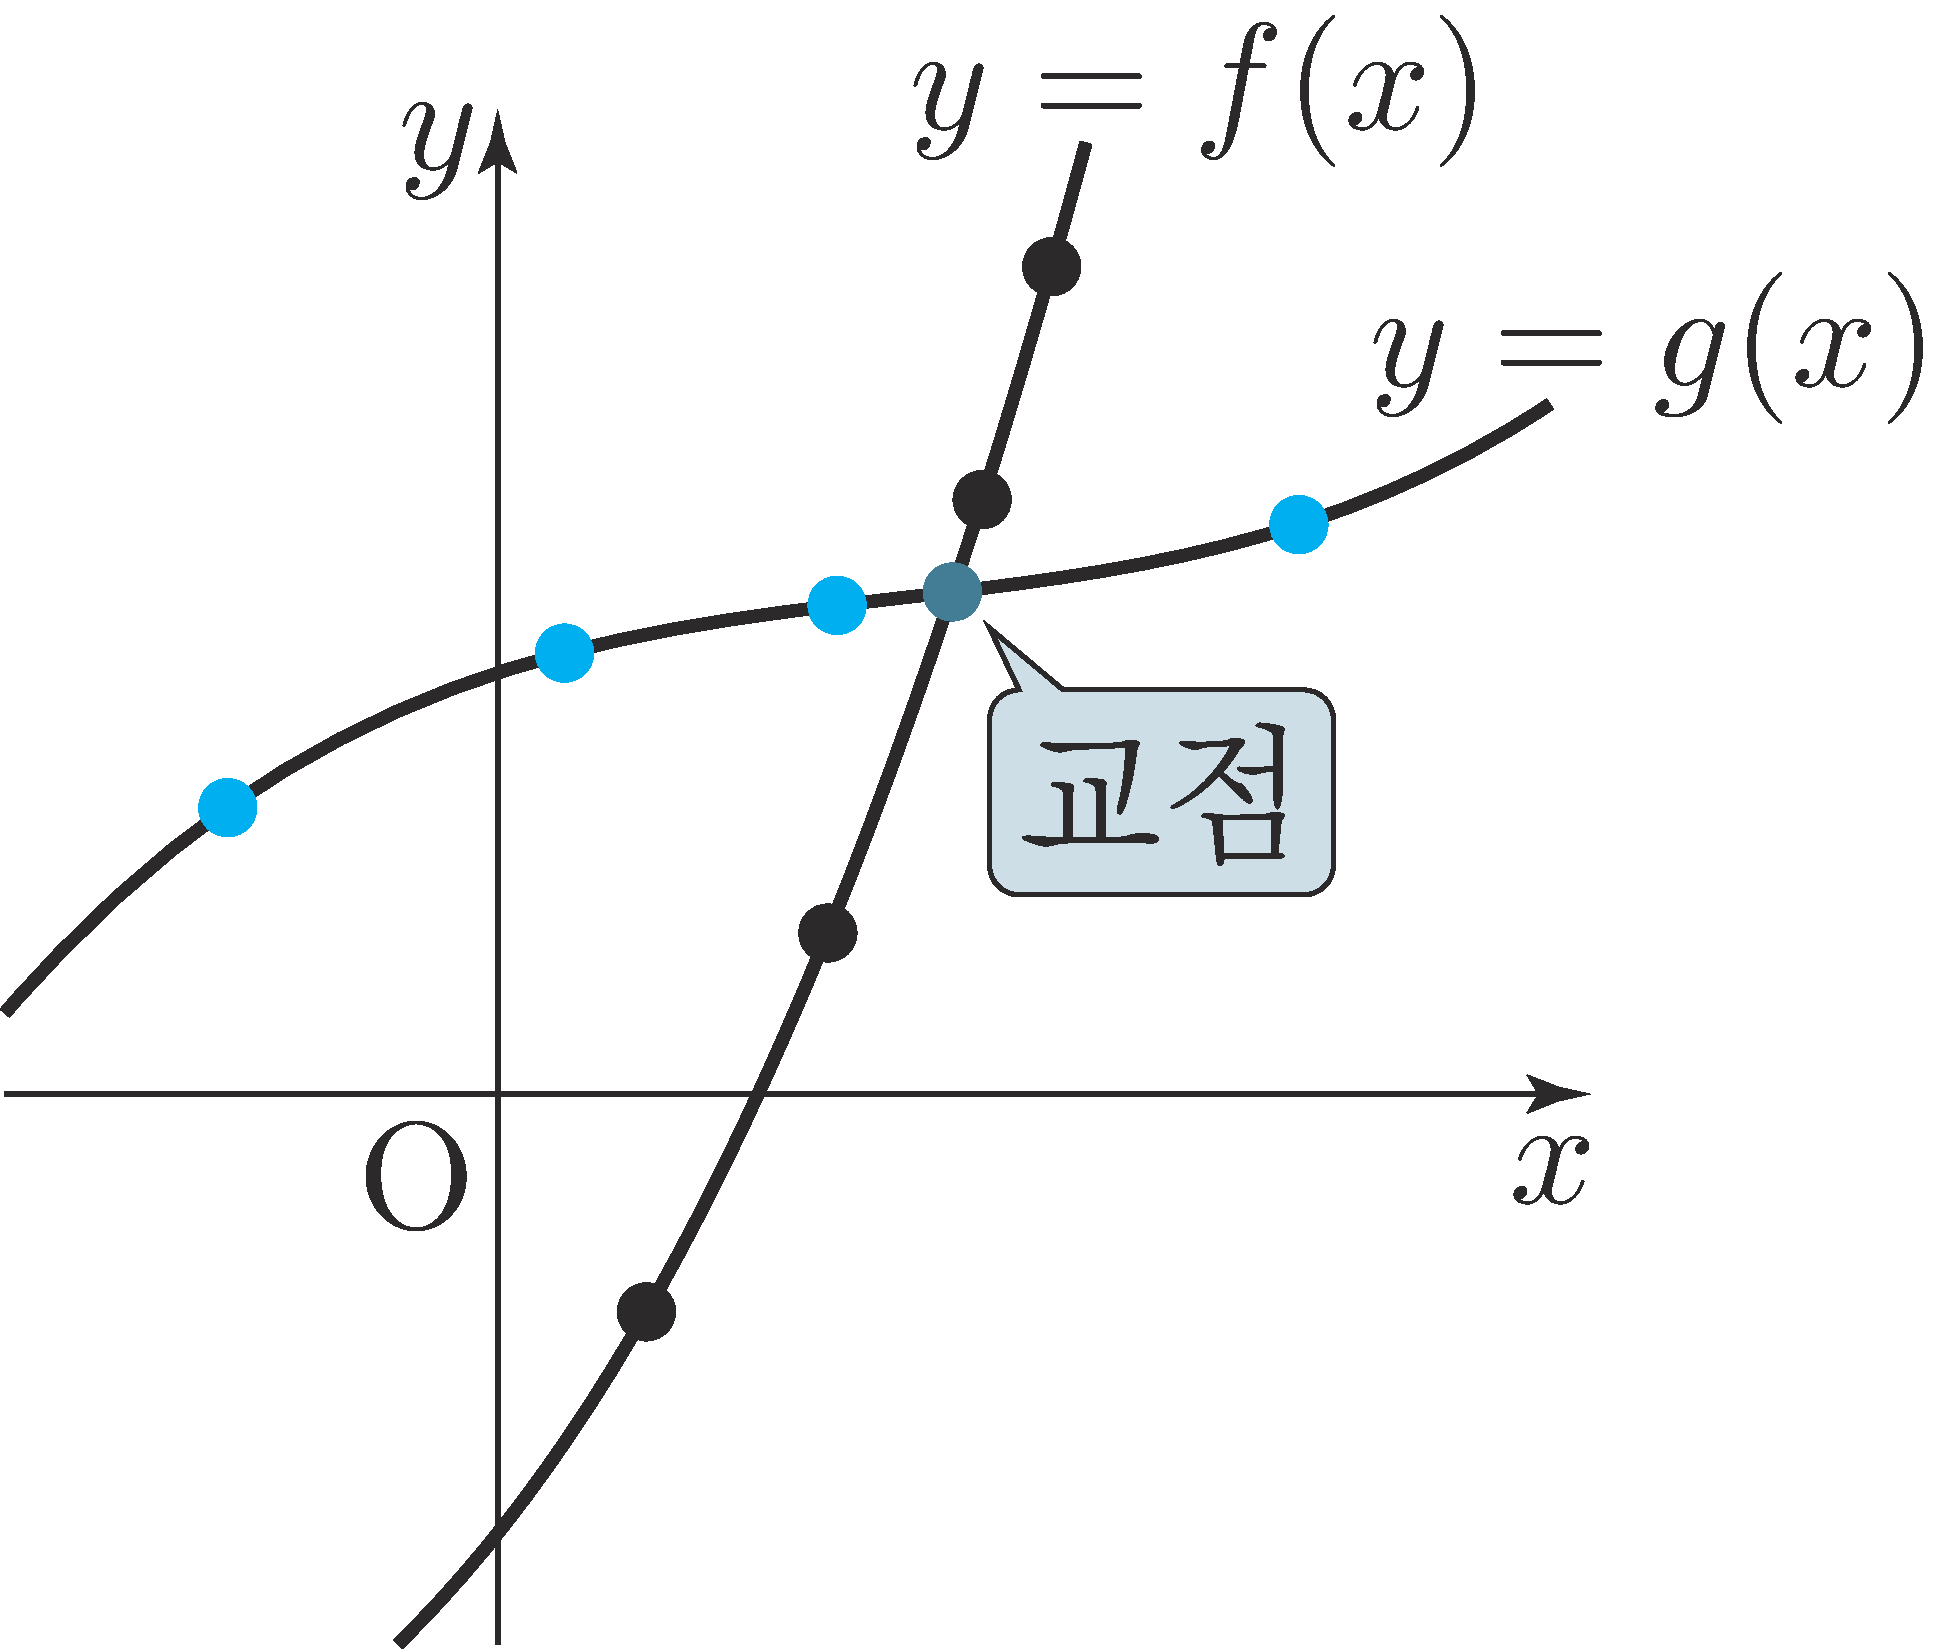
\includegraphics[scale=\pgfkeysvalueof{picsize}]{DBs/pic/zery_18.pdf}\
	\end{center}방정식 $f\left( x \right)= g\left( x \right) $의 (서로 다른) 실근을 그래프를 통해 해석해봅시다.
검은색 점들은 $y=f\left( x \right) $ 위의 점이므로 각각 `$x$좌표가 $x$일 때 $y$좌표가 $f\left( x \right) $인 점'이고, 분홍색 점들은 $y=g\left( x \right) $ 위의 점이므로 `$x$좌표가 $x$일 때 $y$좌표가 $g\left( x \right) $인 점'입니다. 이때 교점은 `$x$좌표가 $x$일 때 $y$좌표가 $f\left( x \right) $이기도 하고 $g\left( x \right) $이기도 한 점'이 됩니다. 따라서 $f\left( x \right) = g\left( x \right) $를 만족하는 점이 두 그래프의 교점입니다.
\begin{center} 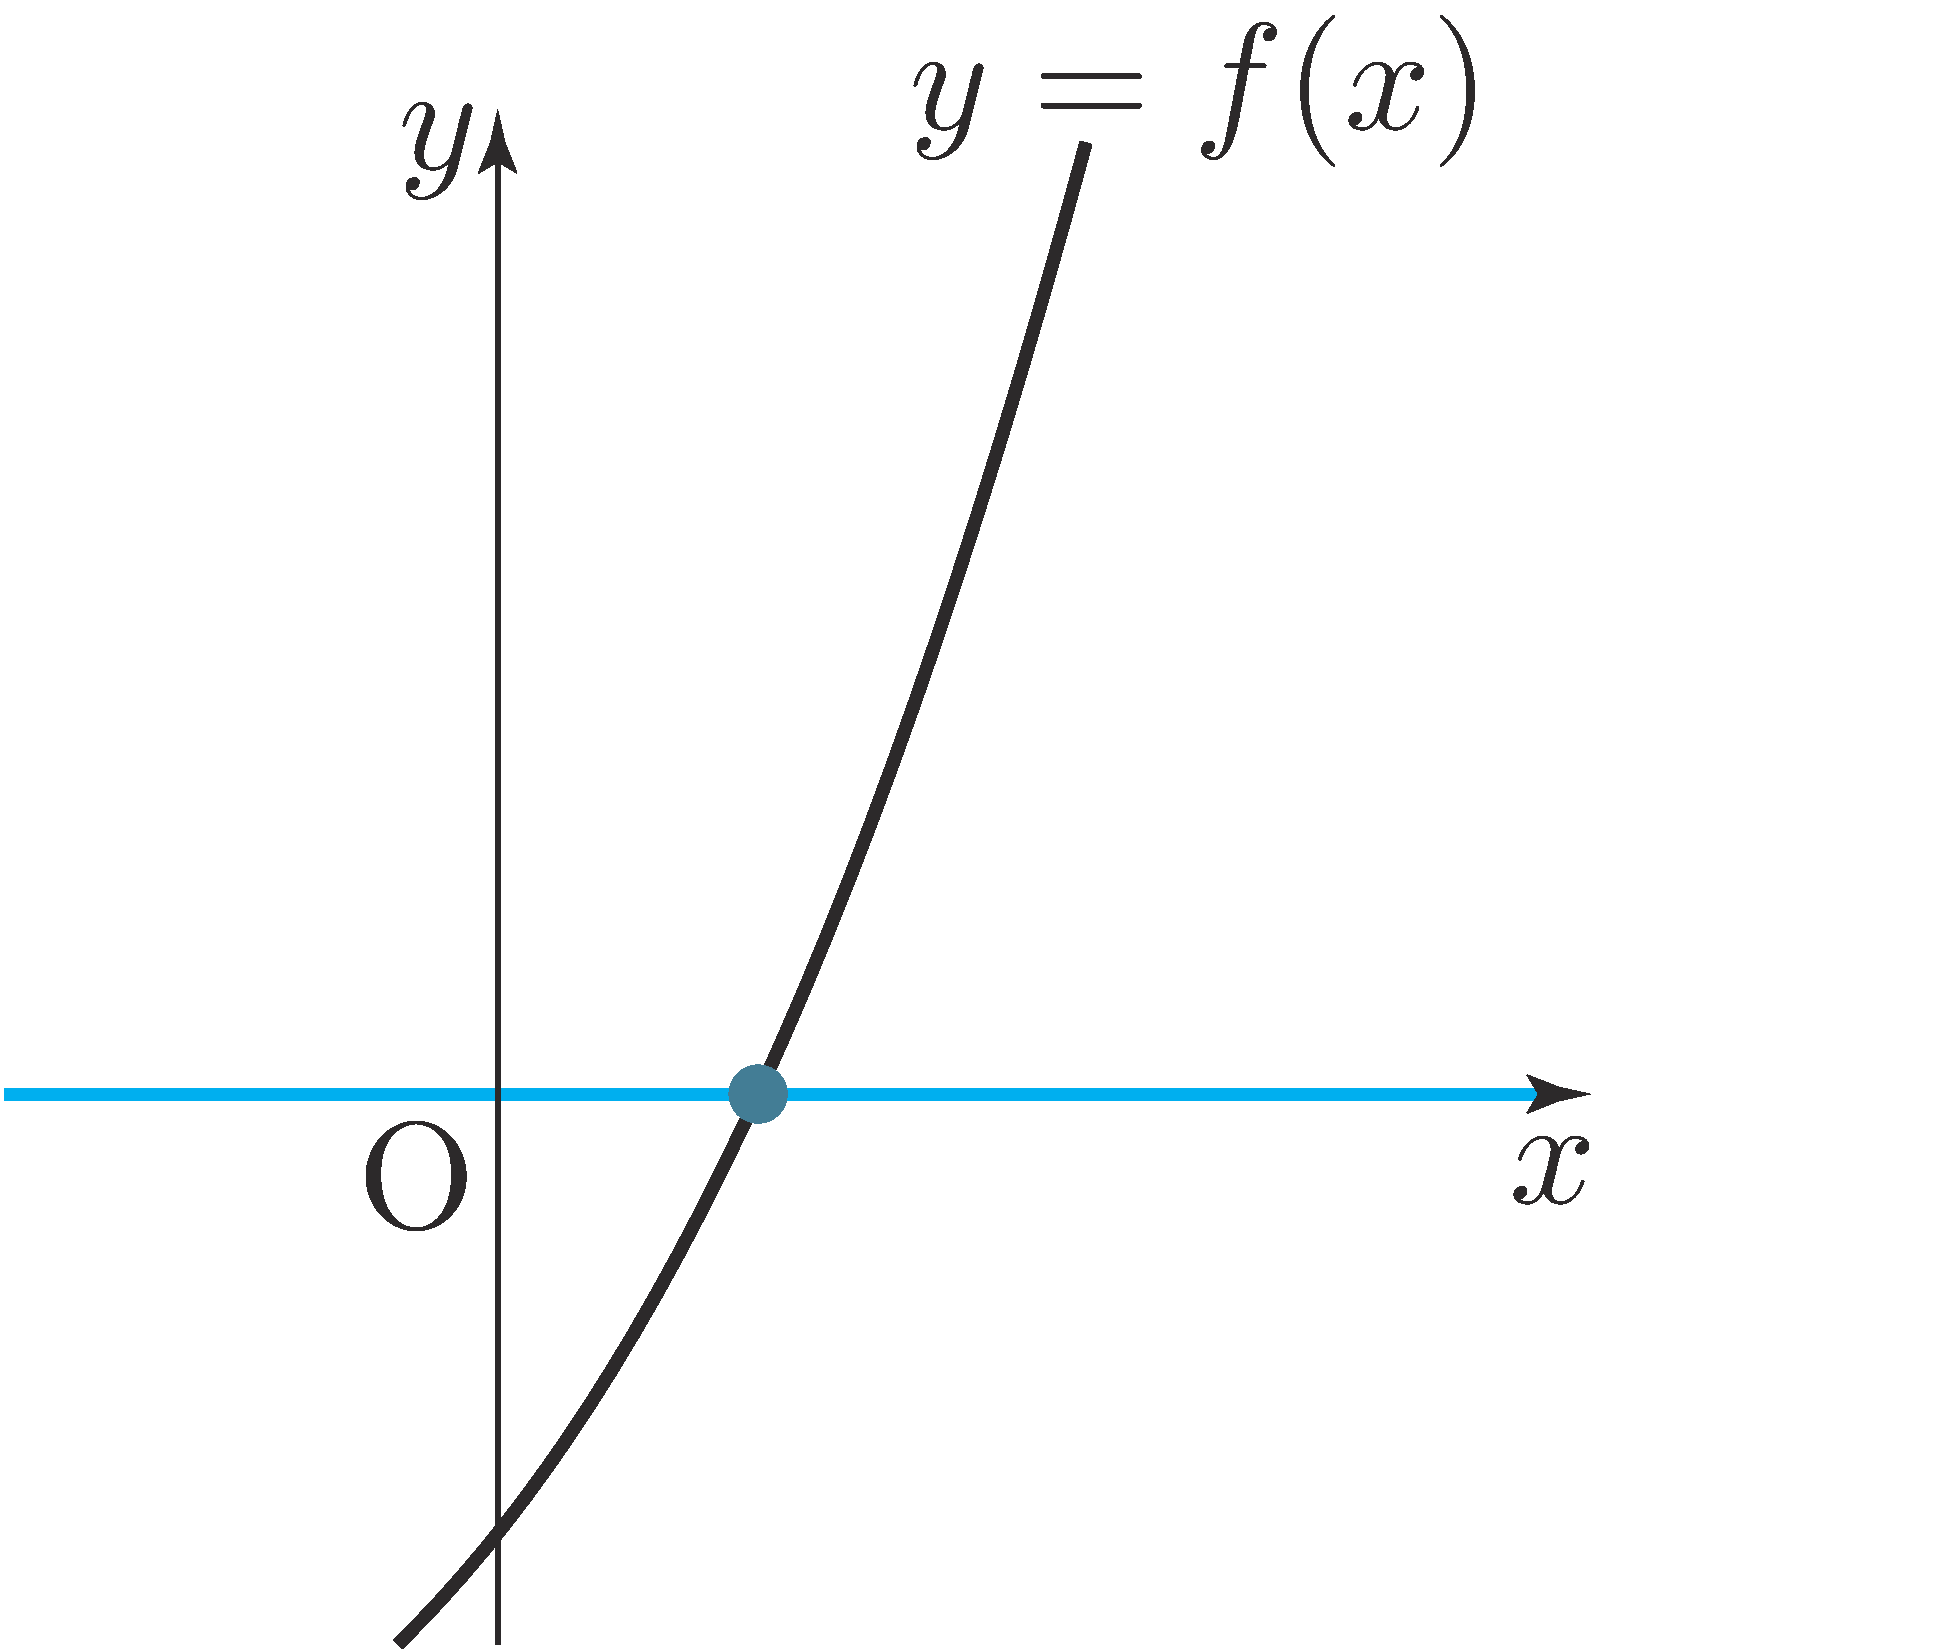
\includegraphics[scale=\pgfkeysvalueof{picsize}]{DBs/pic/zery_19.pdf}\
	\end{center}방정식 $f\left( x \right)=0 $은  $g\left( x \right)=0 $인 경우, 즉 $y=g\left( x \right) $의 그래프가 $x$축인 경우로 해석할 수 있습니다. 따라서 $y=f\left( x \right) $와 $x$축의 교점을 찾으면 방정식을 풀이할 수 있습니다.

\section{부등식과 그래프}
\begin{center} 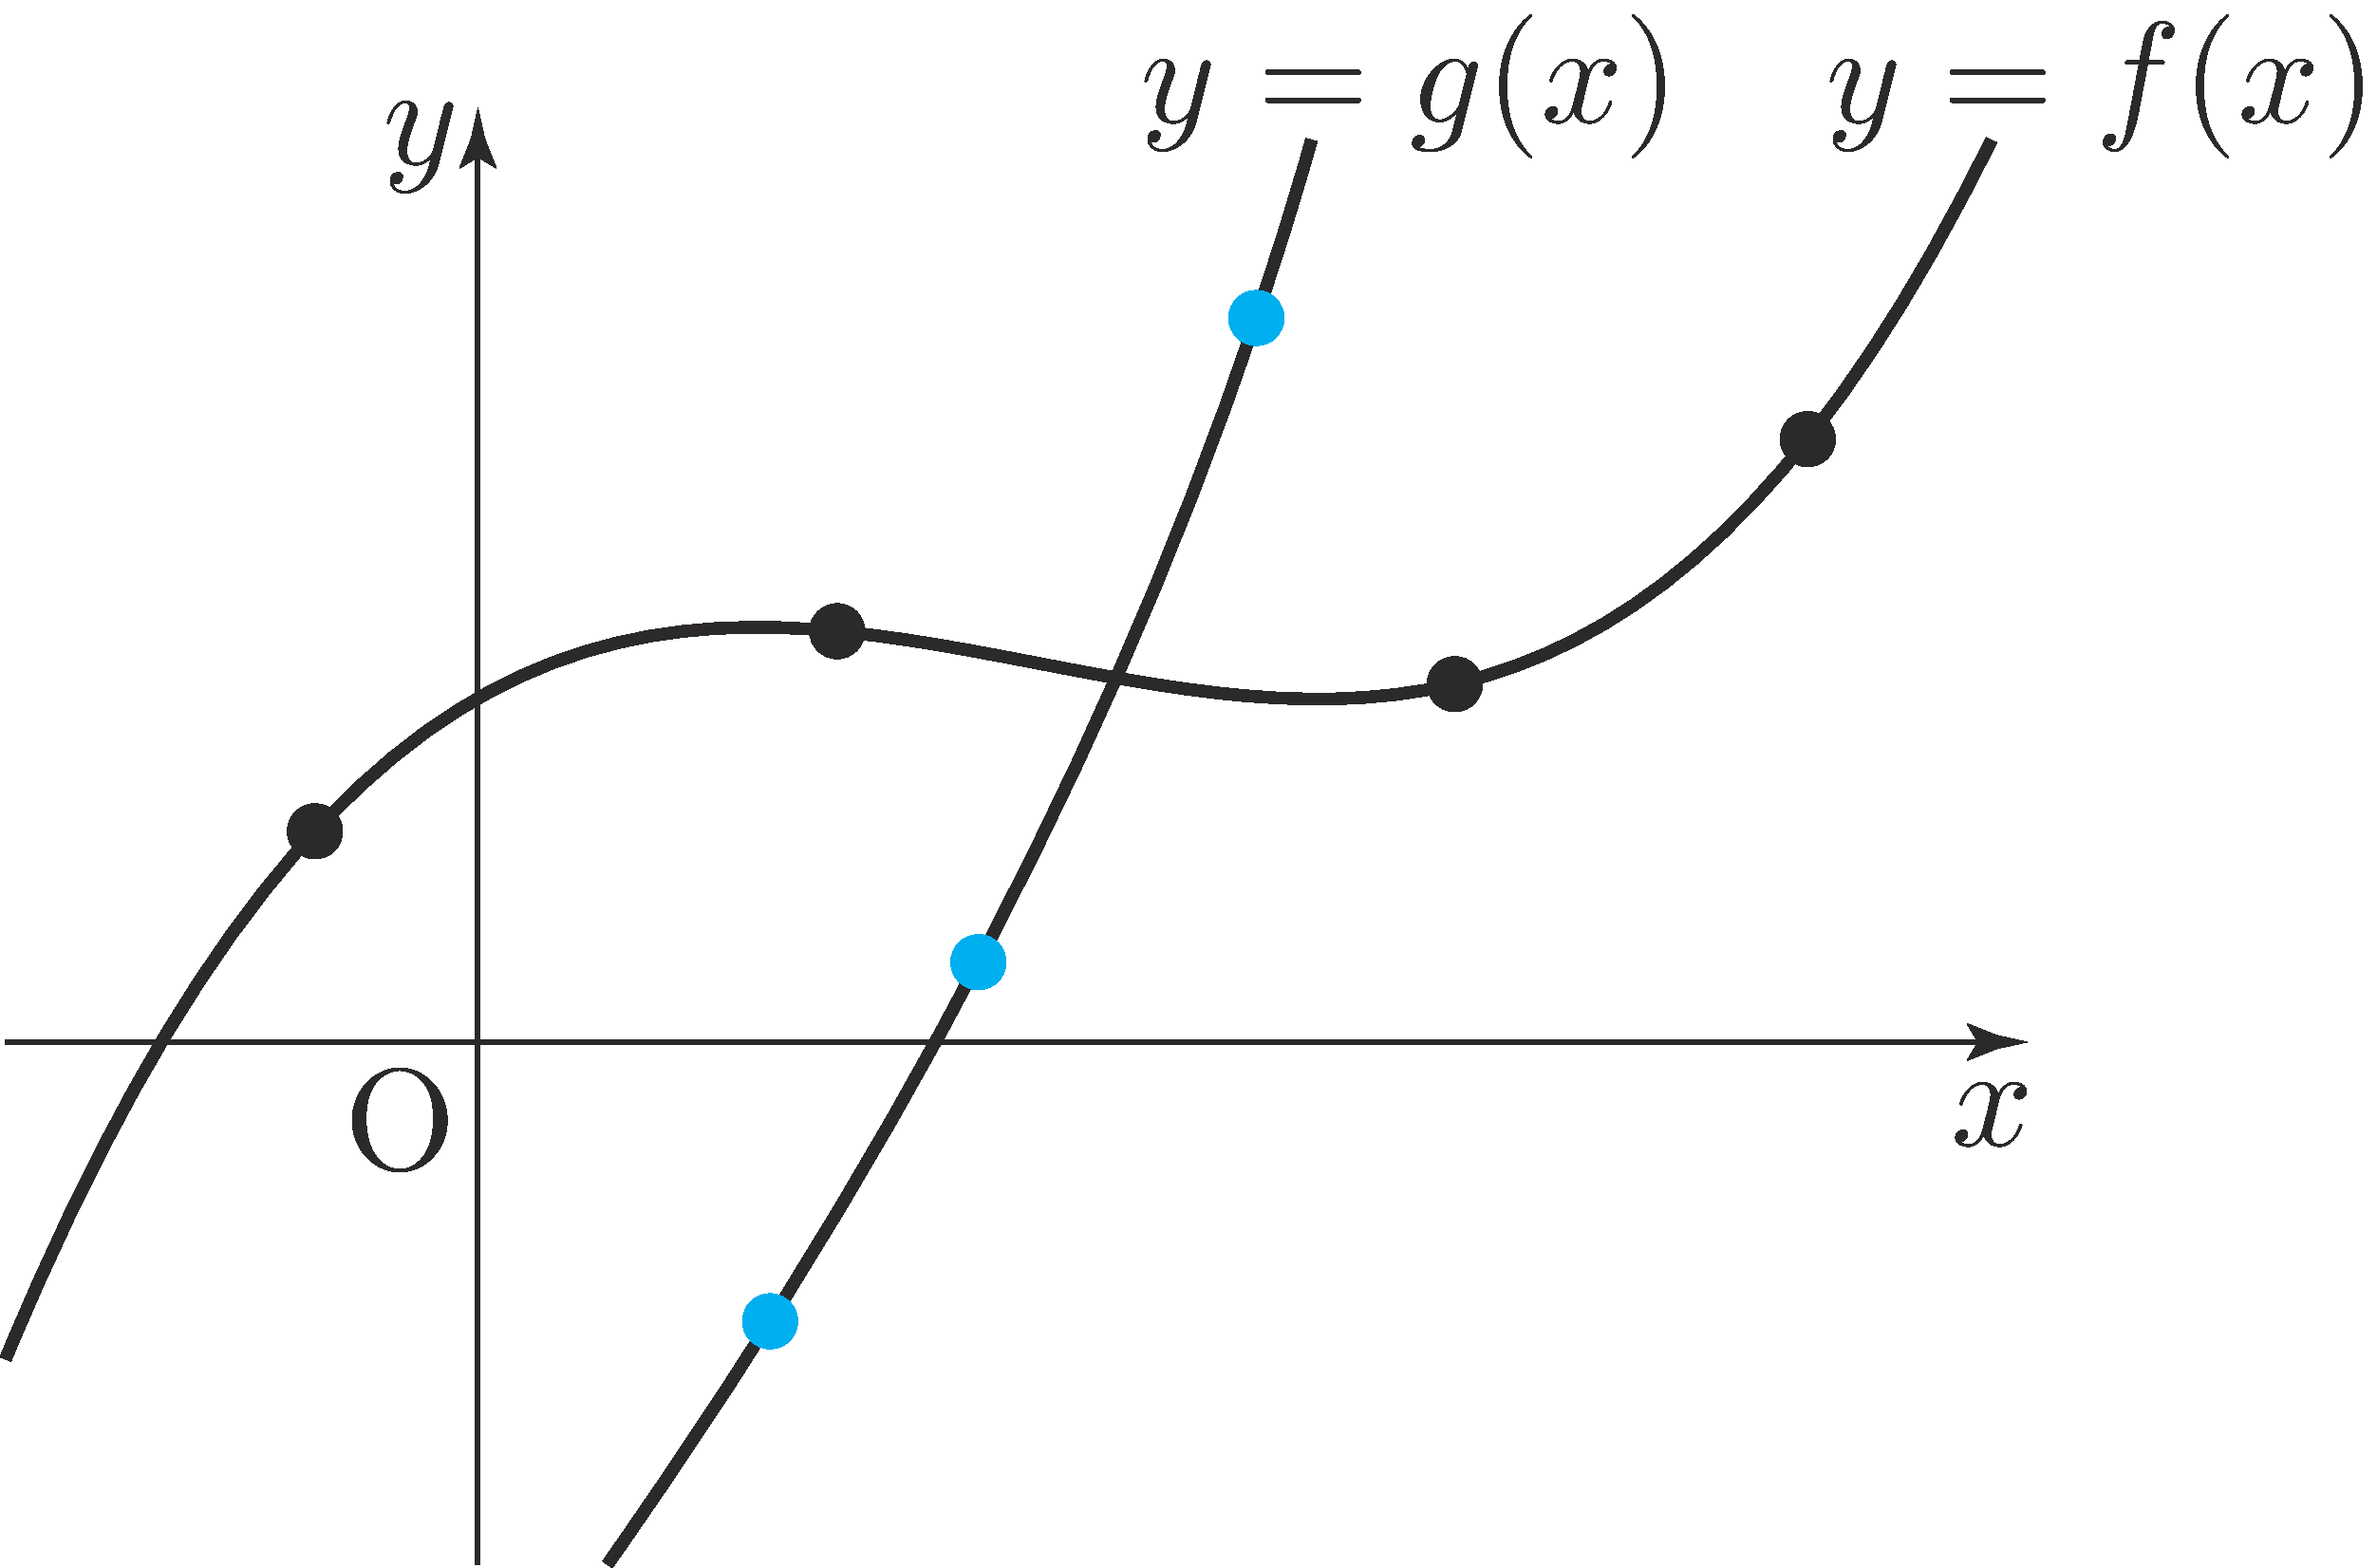
\includegraphics[scale=\pgfkeysvalueof{picsize}]{DBs/pic/zery_20.pdf}\
	\end{center}부등식 $f\left( x \right) > g\left( x \right)  $ 또는 $f\left( x \right) < g\left( x \right)  $의 해를 그래프를 통해 해석해봅시다. 검은색 점들은 $y=f\left( x \right) $ 위의 점이므로 각각 `$x$좌표가 $x$일 때 $y$좌표가 $f\left( x \right) $인 점'이고, 분홍색 점들은 $y=g\left( x \right) $ 위의 점이므로 `$x$좌표가 $x$일 때 $y$좌표가 $g\left( x \right) $인 점'입니다. 이때 $x$좌표가 같은 점들을 찾기 위해 직선 $x=k$를 그으면 다음과 같습니다.
	\clearpage
\vskip-10pt
\begin{center} 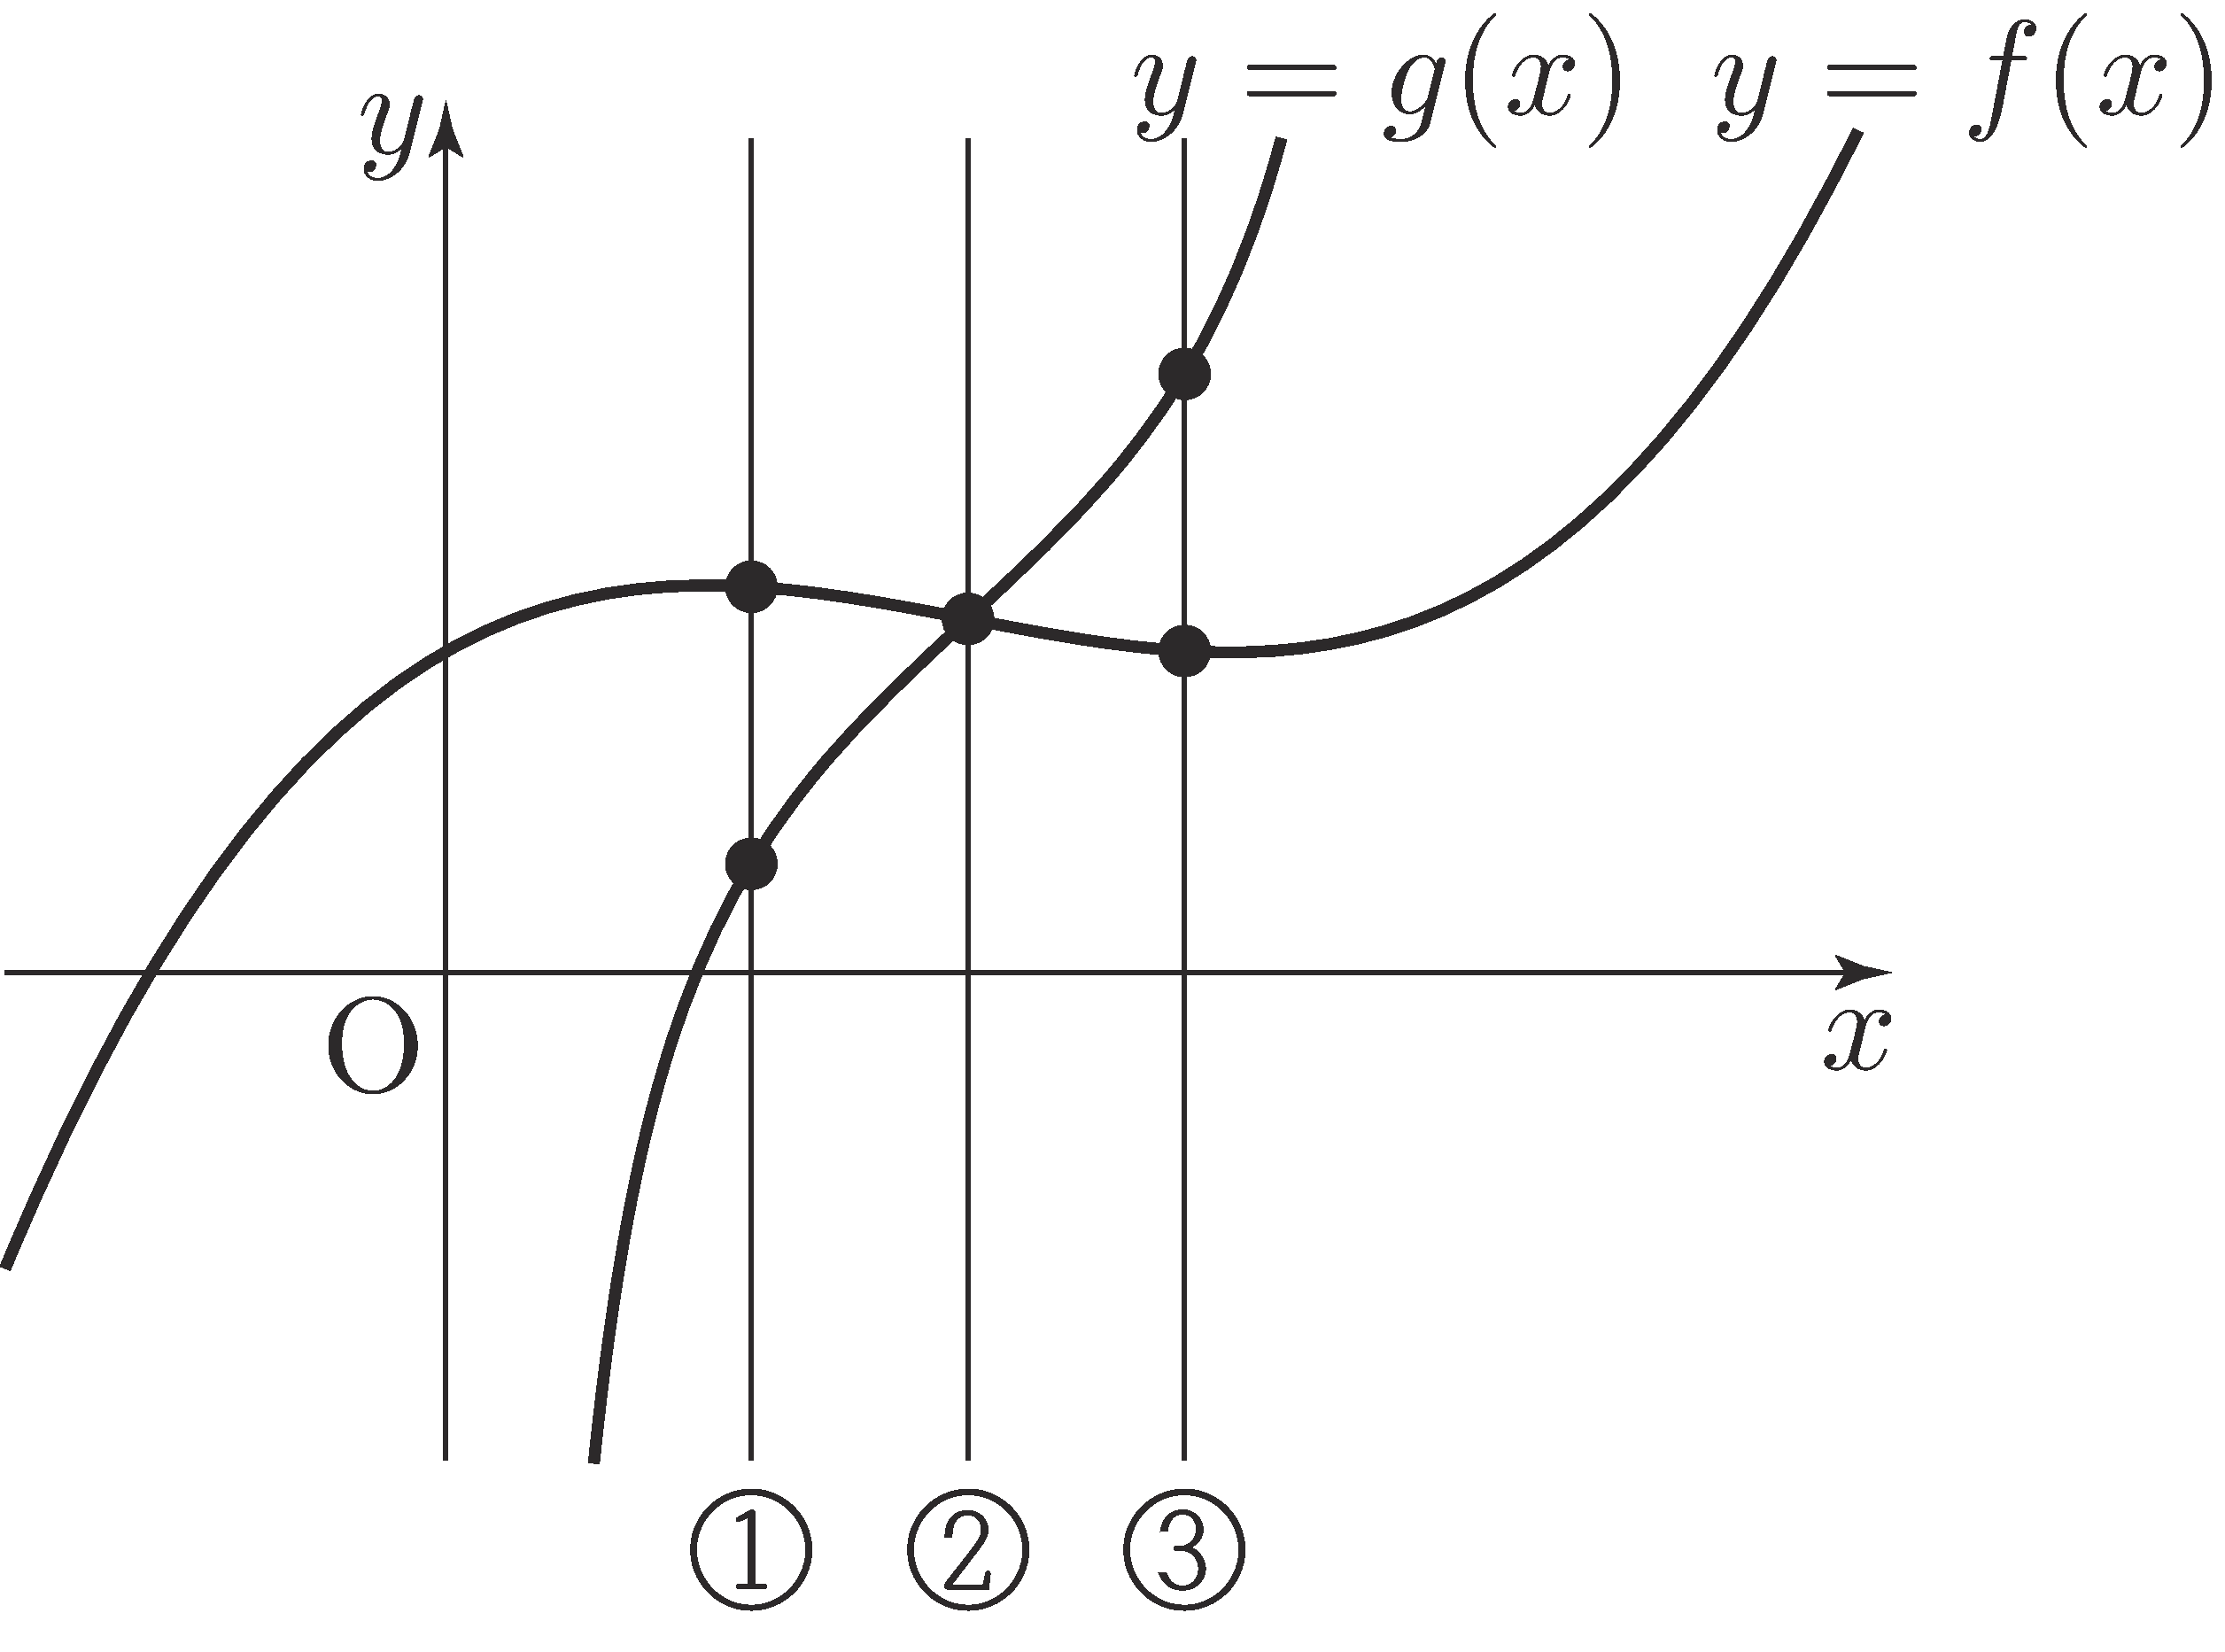
\includegraphics[scale=\pgfkeysvalueof{picsize}]{DBs/pic/zery_21.pdf}\
	\end{center}①에서는 $f\left( x \right) > g\left( x \right) $이고, ②에서는 $f\left( x \right) = g\left( x \right) $이고, ③에서는 $f\left( x \right) < g\left( x \right) $입니다. 즉 위쪽에 그려진 그래프가 같은 $x$ 좌표를 가질 때 $y$좌표가 더 큽니다. 이를 통해 대소를 비교하여 부등식을 풀이할 수 있습니다.
\begin{center} 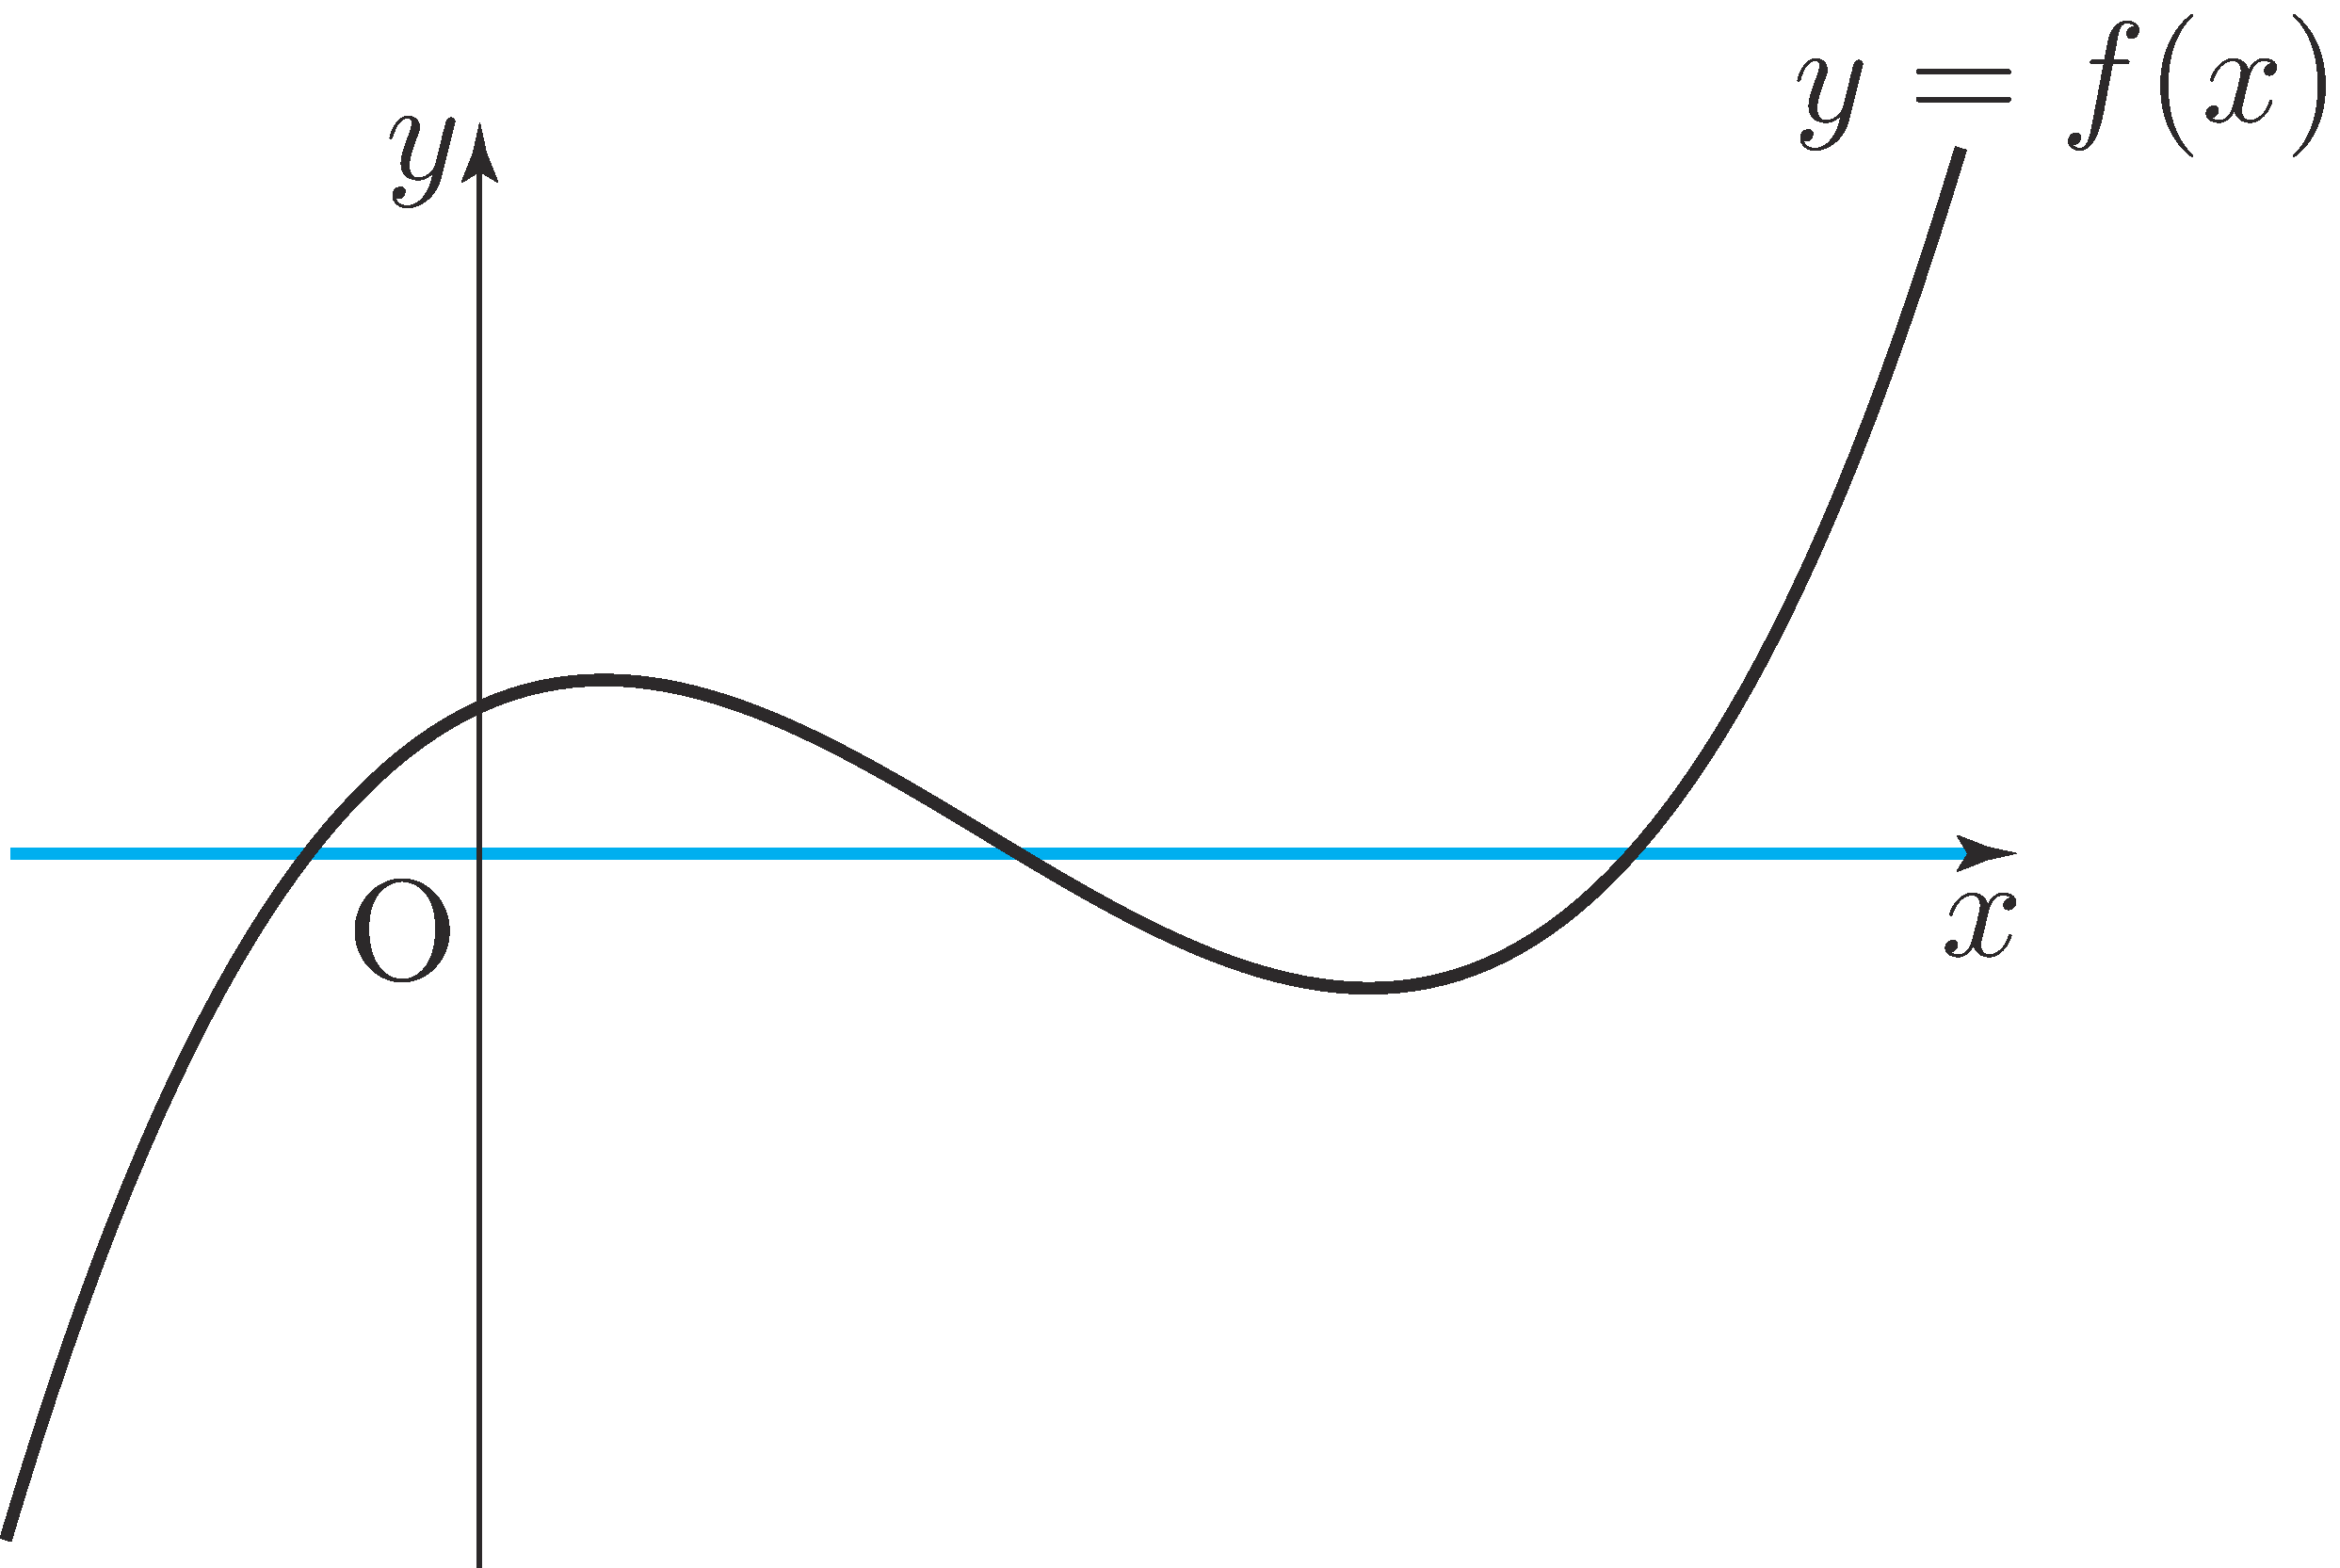
\includegraphics[scale=\pgfkeysvalueof{picsize}]{DBs/pic/zery_22.pdf}\
	\end{center}부등식 $f\left( x \right) > 0$ 또는 $f\left( x \right) <0 $은 $g\left( x \right)=0 $인 경우, 즉 $y=g\left( x \right) $의 그래프가 \mbox{$x$축인} 경우로 해석할 수 있습니다. 따라서 $y=f\left( x \right) $와 $x$축 중 누가 위쪽에 있는지를 따져 부등식을 풀이할 수 있습니다.\vskip-10pt



\section{이차함수의 그래프와 이차부등식}
\subsection{이차함수의 그래프}
\begin{figure}[h]\centering \subfloat[][]{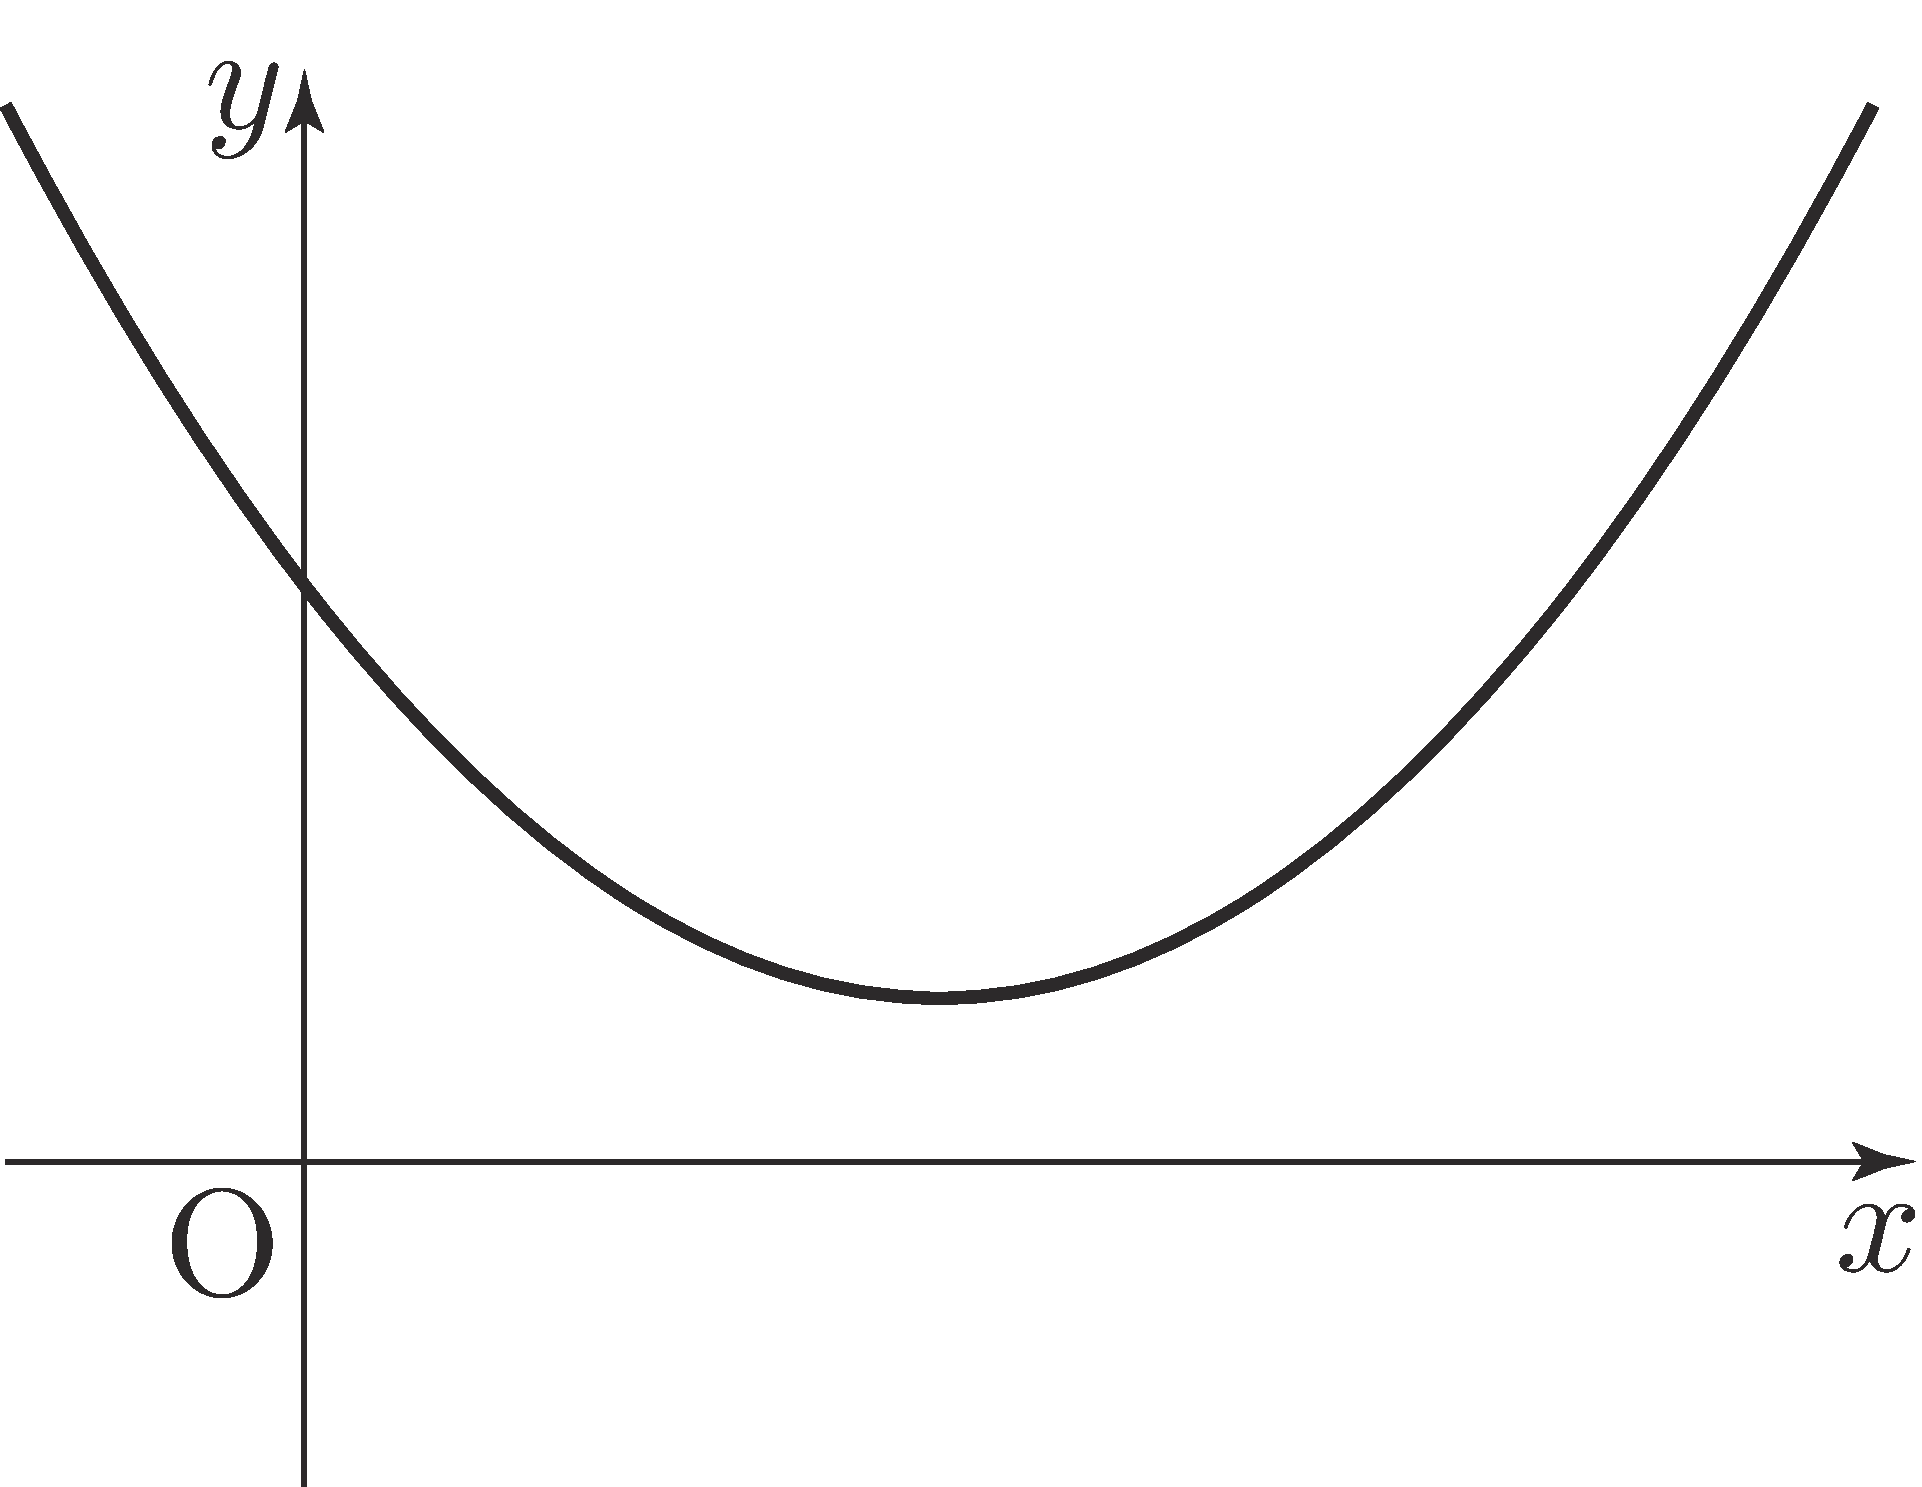
\includegraphics[scale=\pgfkeysvalueof{picsize}]{DBs/pic/zery_23_1.pdf}}\
\qquad\qquad
\centering \subfloat[][]{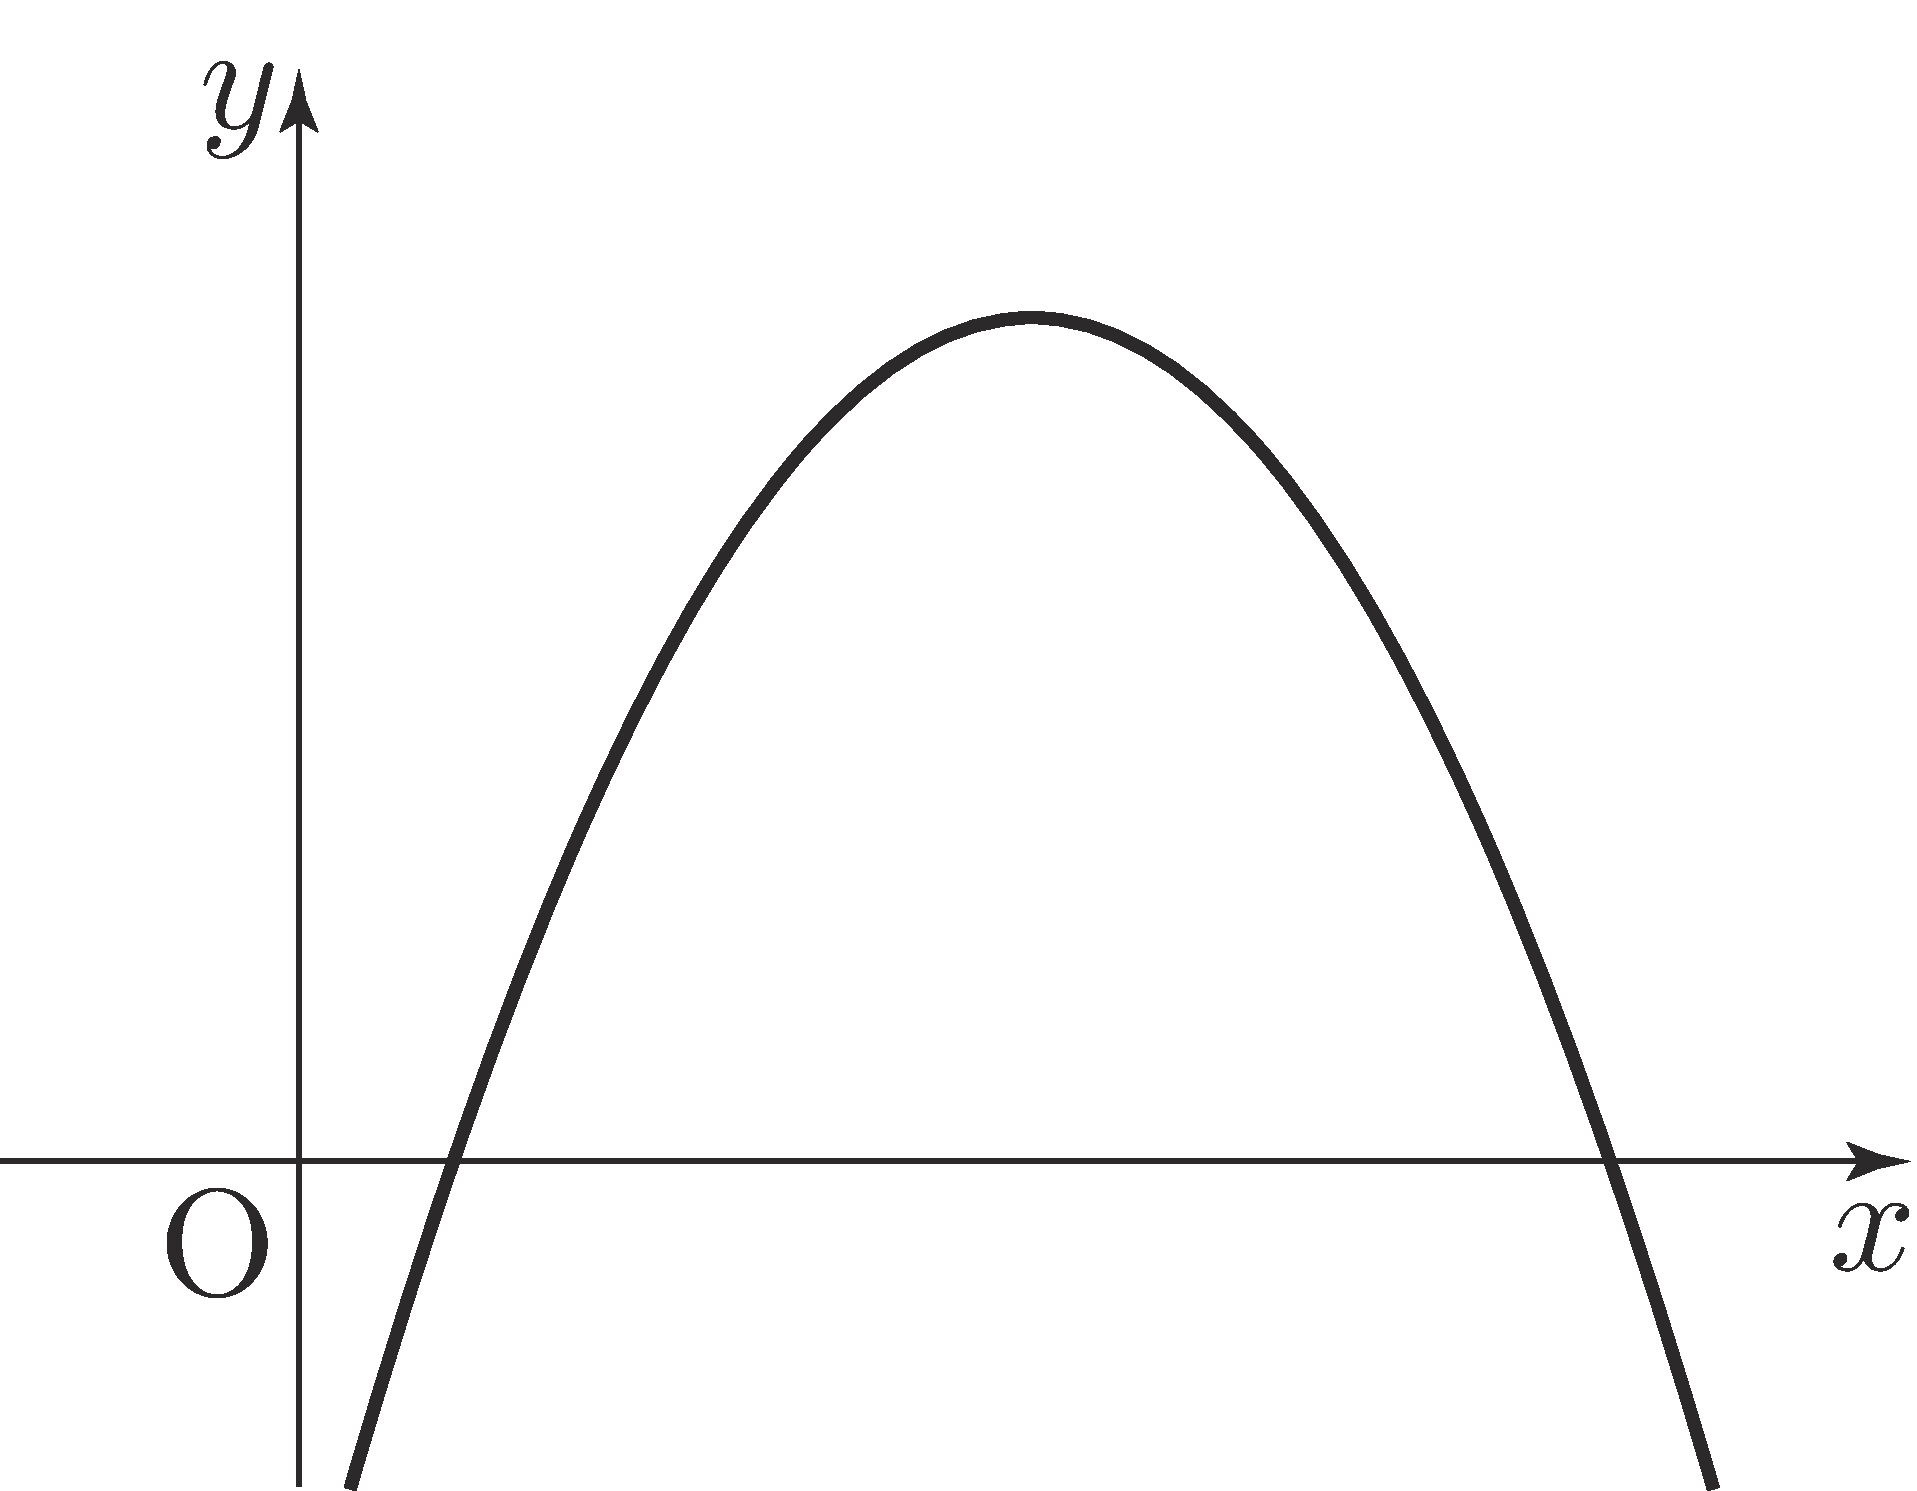
\includegraphics[scale=\pgfkeysvalueof{picsize}]{DBs/pic/zery_23_2.pdf}}\
\end{figure}

최고차항인 이차항의 계수 $a$의 부호에 따라 이차함수의 그래프의 모양이 달라집니다. $a>0$이면 (a)와 같으며, 이러한 모양을 \term{아래로 볼록하다}{}고 합니다. $a<0$이면 (b)와 같으며, 이러한 모양을 \term{위로 볼록하다}{}고 합니다. \vskip-10pt

\subsection{이차부등식의 풀이}
이차부등식은 다음의 네 부등식 중 하나입니다. (단, $a \ne 0$)
\begin{align*}
	&ax^2 + bx + c > 0, \quad ax^2 + bx + c \ge 0, \\
	&ax^2 + bx + c < 0, \quad ax^2 + bx + c \le 0  
\end{align*}
\clearpage
$D>0$일 때 이차방정식 $ax^2 + bx + c=0$의 두 근을 각각 $\alpha$, $\beta$ $(\alpha<\beta)$라 하고, $D=0$일 때 이차방정식의 한 근(중근)을 $\gamma$라 합시다. 이제 이차부등식을 그래프로 풀이하며 수식을 통한 풀이와 연관지어 생각해봅시다. 
\subsubsection{$ax^2 + bx + c > 0$}
\begin{center} 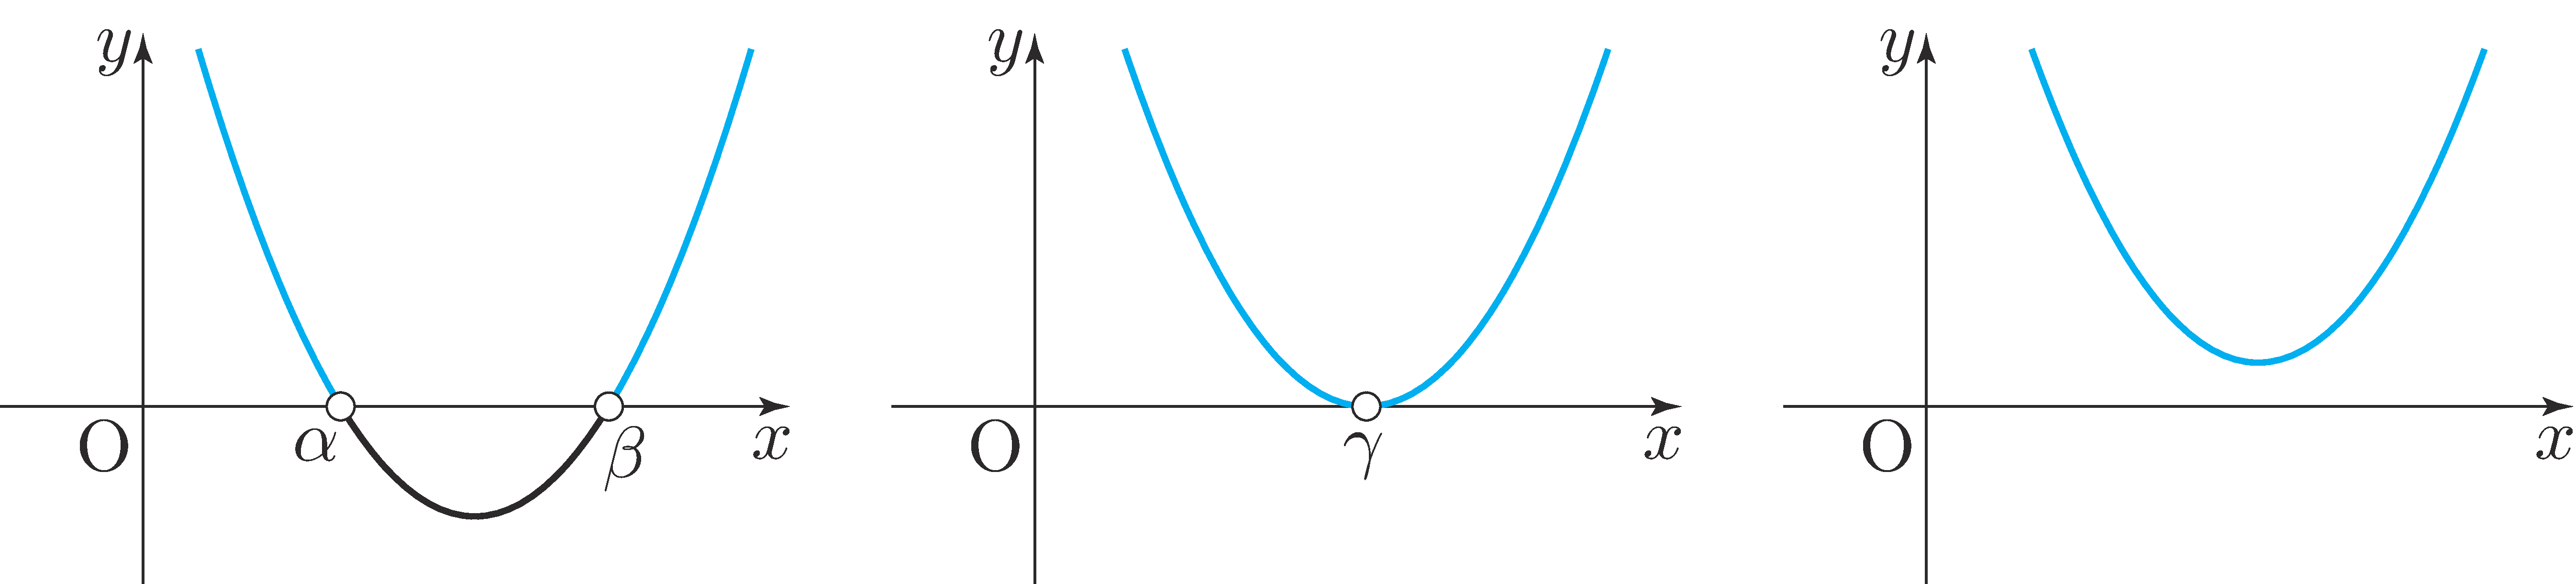
\includegraphics[scale=\pgfkeysvalueof{picsize}]{DBs/pic/zery_24.pdf}\
	\end{center}$a>0$일 때, $D>0$이면 $\OOI{-\infty}{\alpha}$, $\OOI{\beta}{\infty}$에 포함된 모든 실수가 부등식의 해입니다. $D=0$이면 $\OOI{-\infty}{\gamma}$, $\OOI{\gamma}{\infty}$에 포함된 모든 실수가 부등식의 해이므로, $\gamma$가 아닌 모든 실수가 부등식의 해입니다.  $D<0$이면 모든 실수가 부등식의 해입니다.
\begin{center} 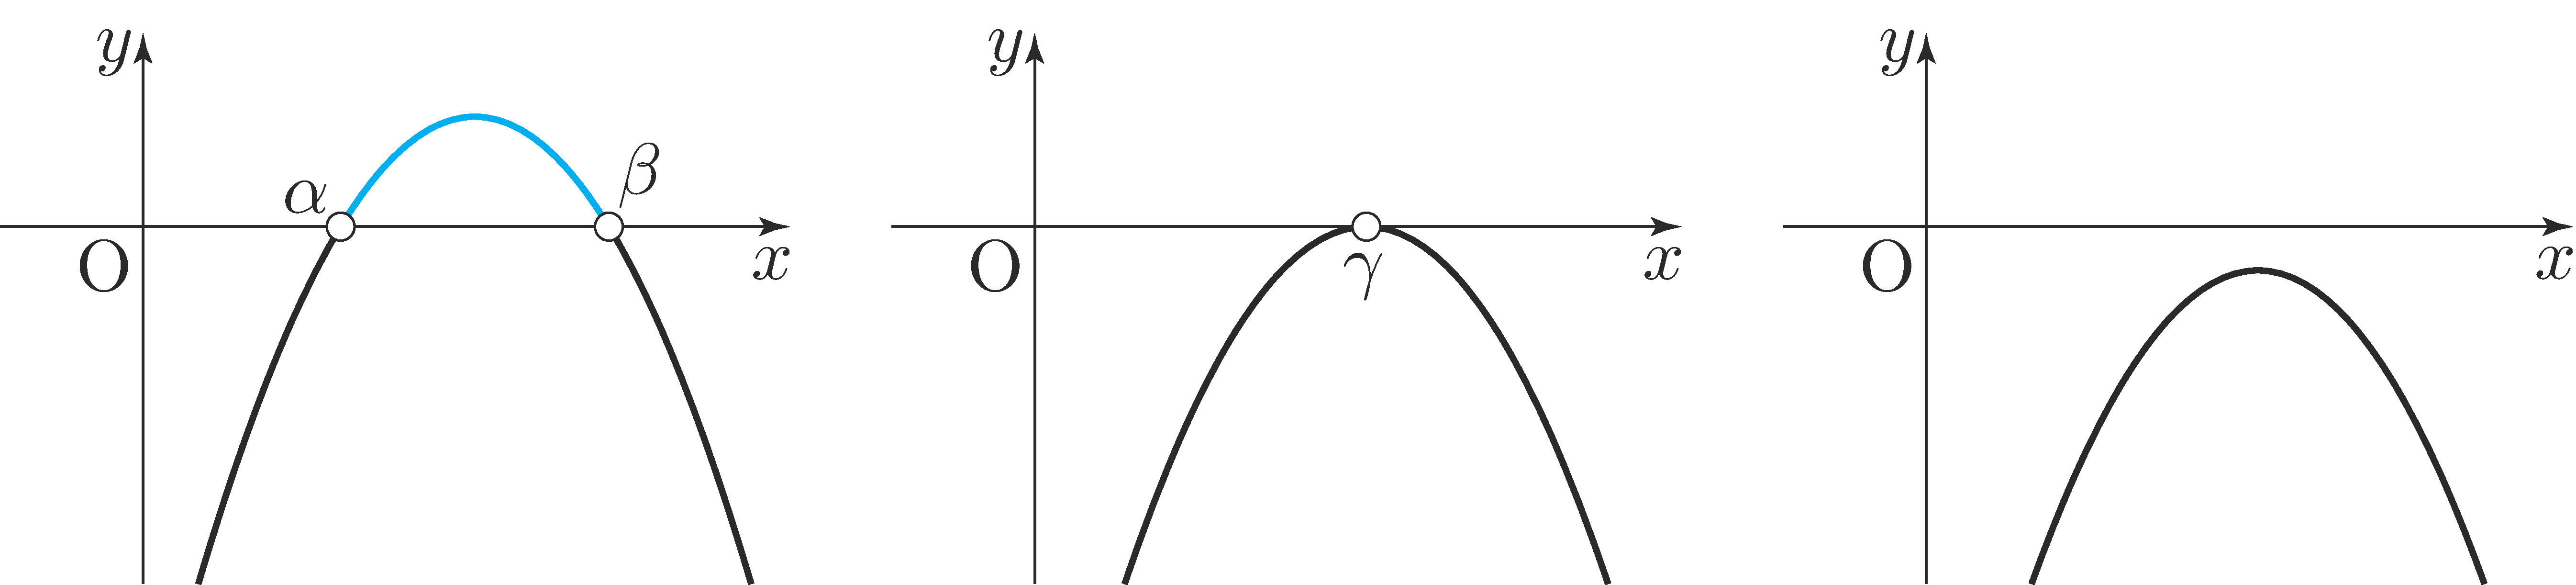
\includegraphics[scale=\pgfkeysvalueof{picsize}]{DBs/pic/zery_24_1.pdf}\
	\end{center}$a<0$일 때, $D>0$이면 $\OOI{\alpha}{\beta}$에 포함된 모든 실수가 부등식의 해입니다. $D=0$이면 부등식의 해가 없습니다. $D<0$이면 부등식의 해가 없습니다.
\subsubsection{$ax^2 + bx + c \ge 0$}
\begin{center} 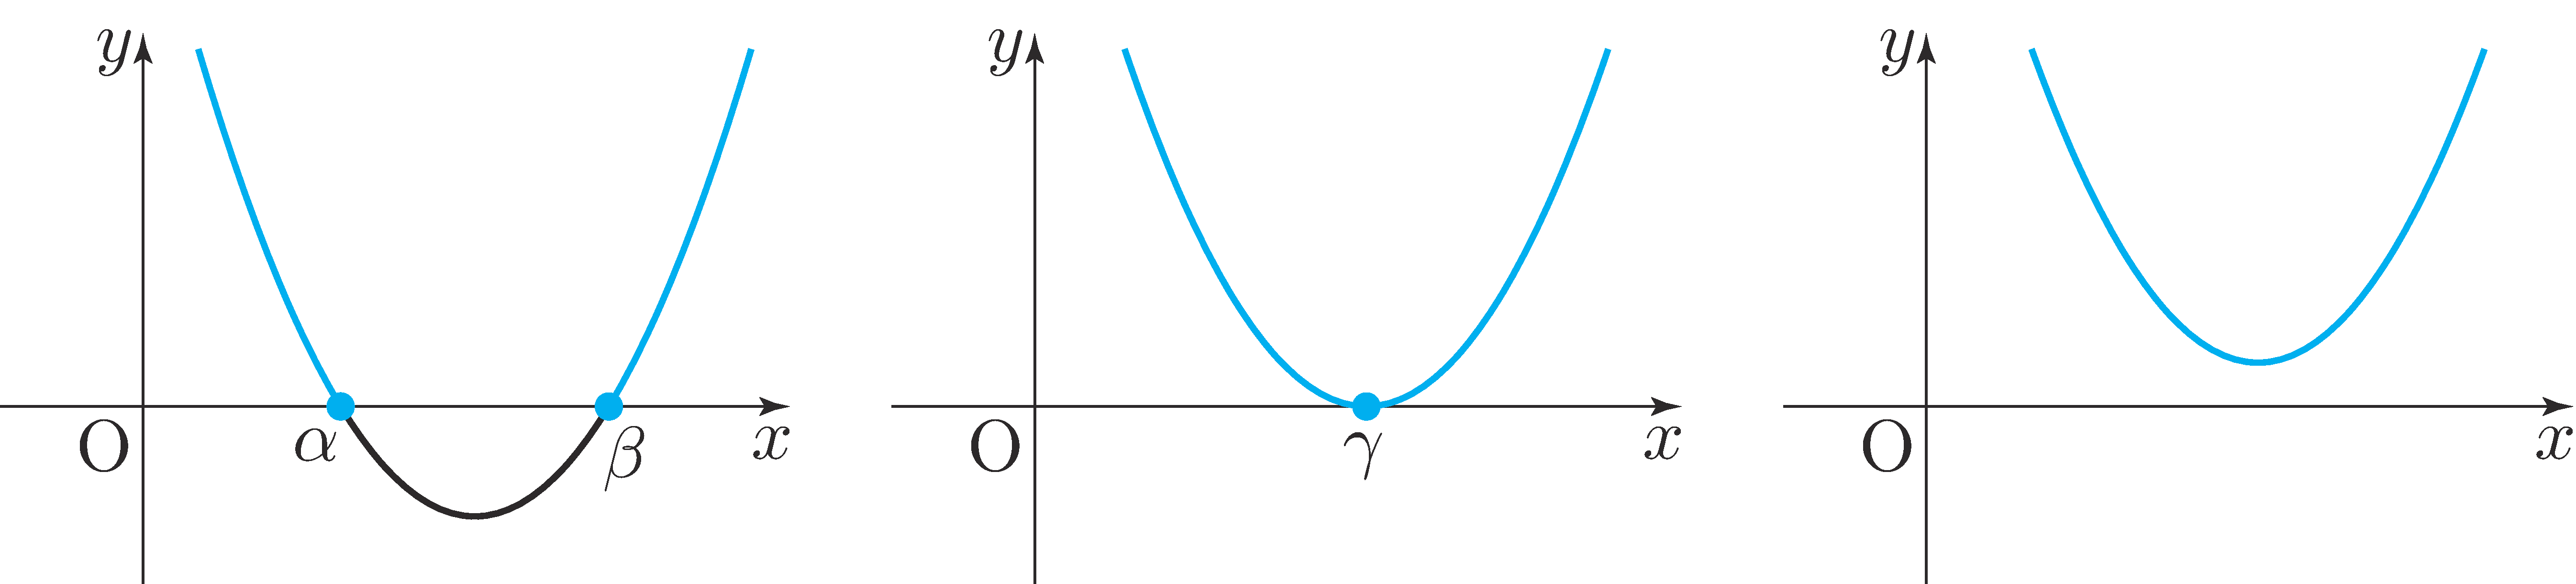
\includegraphics[scale=\pgfkeysvalueof{picsize}]{DBs/pic/zery_25.pdf}\
	\end{center}$a>0$일 때, $D>0$이면 $\OCI{-\infty}{\alpha}$, $\COI{\beta}{\infty}$에 포함된 모든 실수가 부등식의 해입니다. $D=0$이면 $\OCI{-\infty}{\gamma}$, $\OOI{\gamma}{\infty}$에 포함된 모든 실수가 부등식의 해이므로, 모든 실수가 부등식의 해입니다.  $D<0$이면 모든 실수가 부등식의 해입니다.
\begin{center} 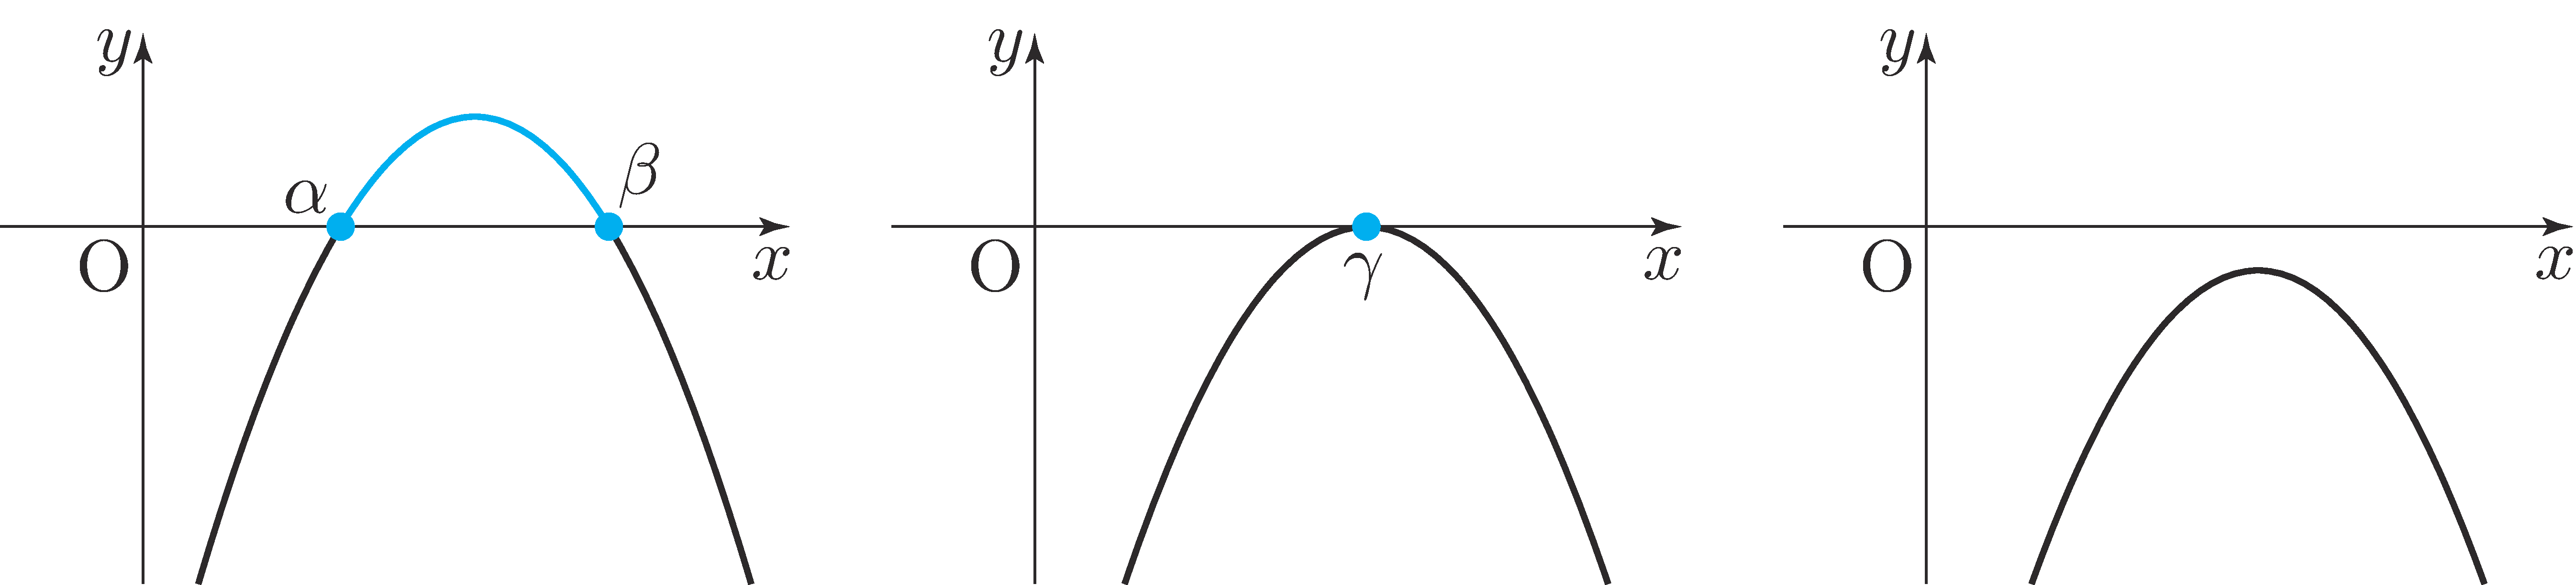
\includegraphics[scale=\pgfkeysvalueof{picsize}]{DBs/pic/zery_25_1.pdf}\
	\end{center}$a<0$일 때, $D>0$이면 $\CCI{\alpha}{\beta}$에 포함된 모든 실수가 부등식의 해입니다. $D=0$이면 $x=\gamma$가 부등식의 해입니다. $D<0$이면 부등식의 해가 없습니다.

\subsubsection{$ax^2 + bx + c < 0$}
\begin{center} 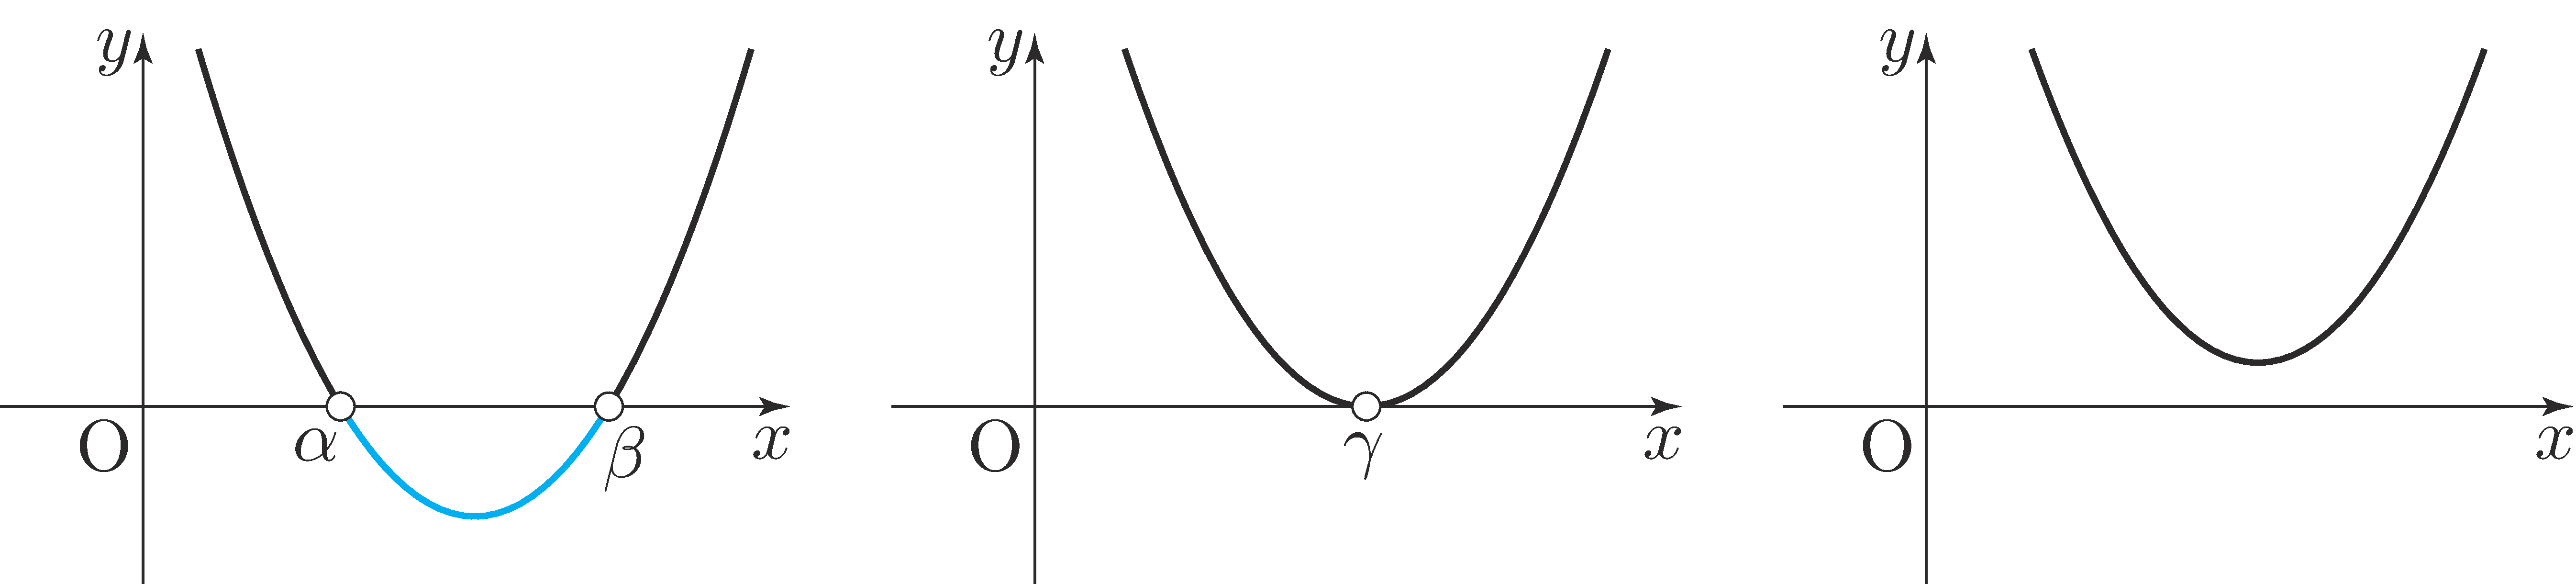
\includegraphics[scale=\pgfkeysvalueof{picsize}]{DBs/pic/zery_26.pdf}\
	\end{center}$a>0$일 때, $D>0$이면 $\OOI{\alpha}{\beta}$에 포함된 모든 실수가 부등식의 해입니다. $D=0$이면 부등식의 해가 없습니다. $D<0$이면 부등식의 해가 없습니다. 
\begin{center} 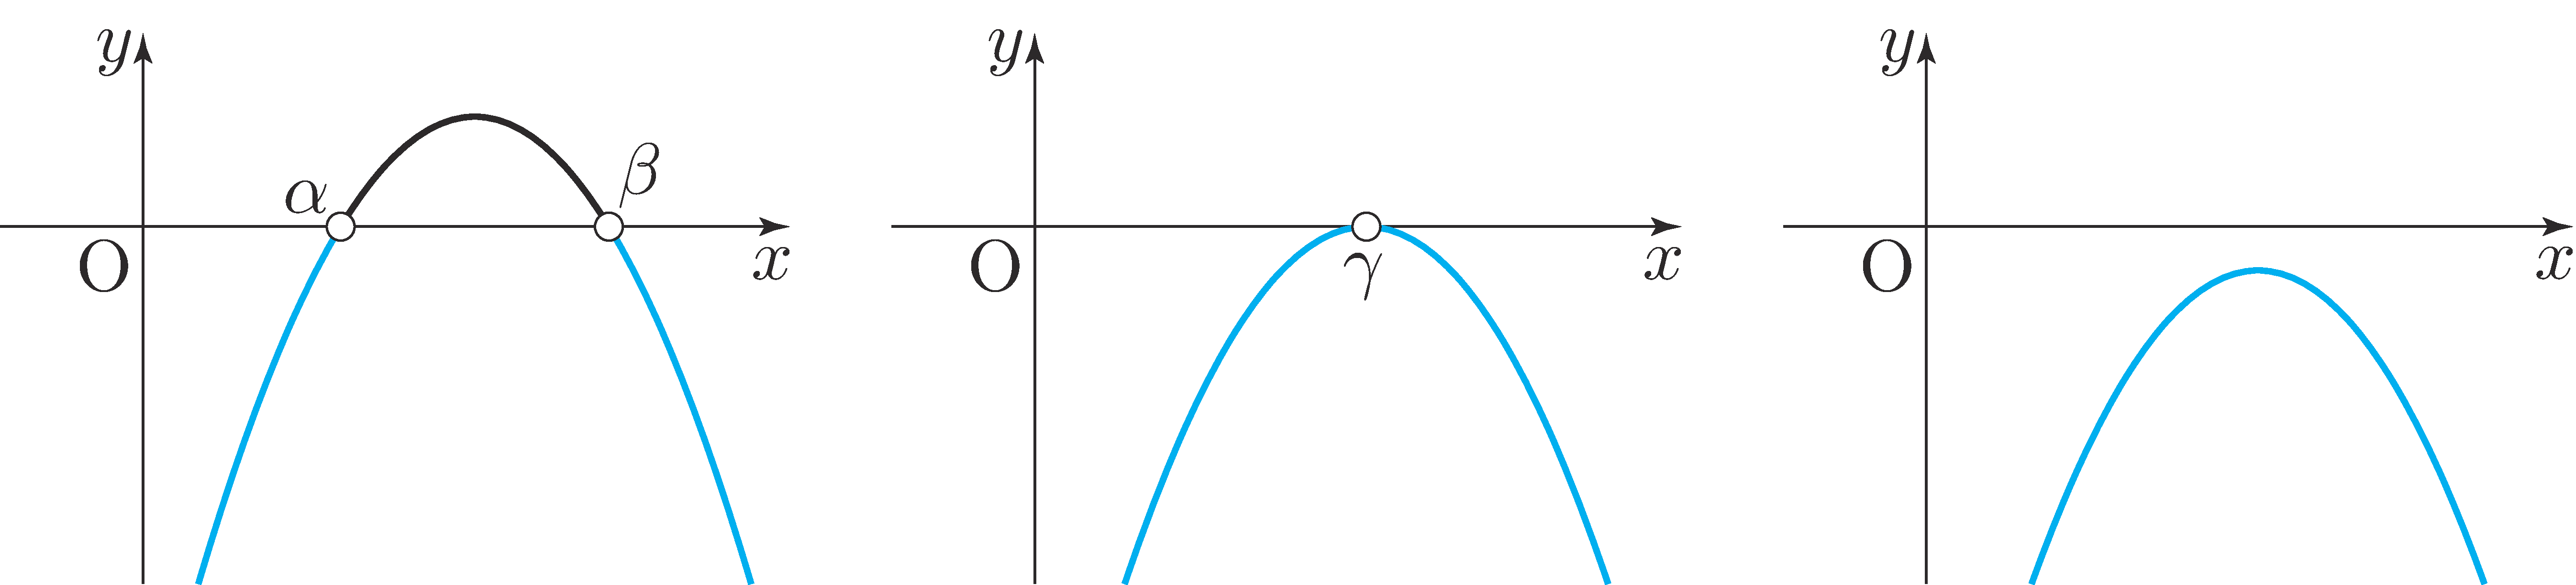
\includegraphics[scale=\pgfkeysvalueof{picsize}]{DBs/pic/zery_26_1.pdf}\
	\end{center}$a<0$일 때, $D>0$이면 $\OOI{-\infty}{\alpha}$, $\OOI{\beta}{\infty}$에 포함된 모든 실수가 부등식의 해입니다. $D=0$이면 $\OOI{-\infty}{\gamma}$, $\OOI{\gamma}{\infty}$에 포함된 모든 실수가 부등식의 해이므로, $\gamma$가 아닌 모든 실수가 부등식의 해입니다. $D<0$이면 모든 실수가 부등식의 해입니다.


\subsubsection{$ax^2 + bx + c \le 0$}
\begin{center} 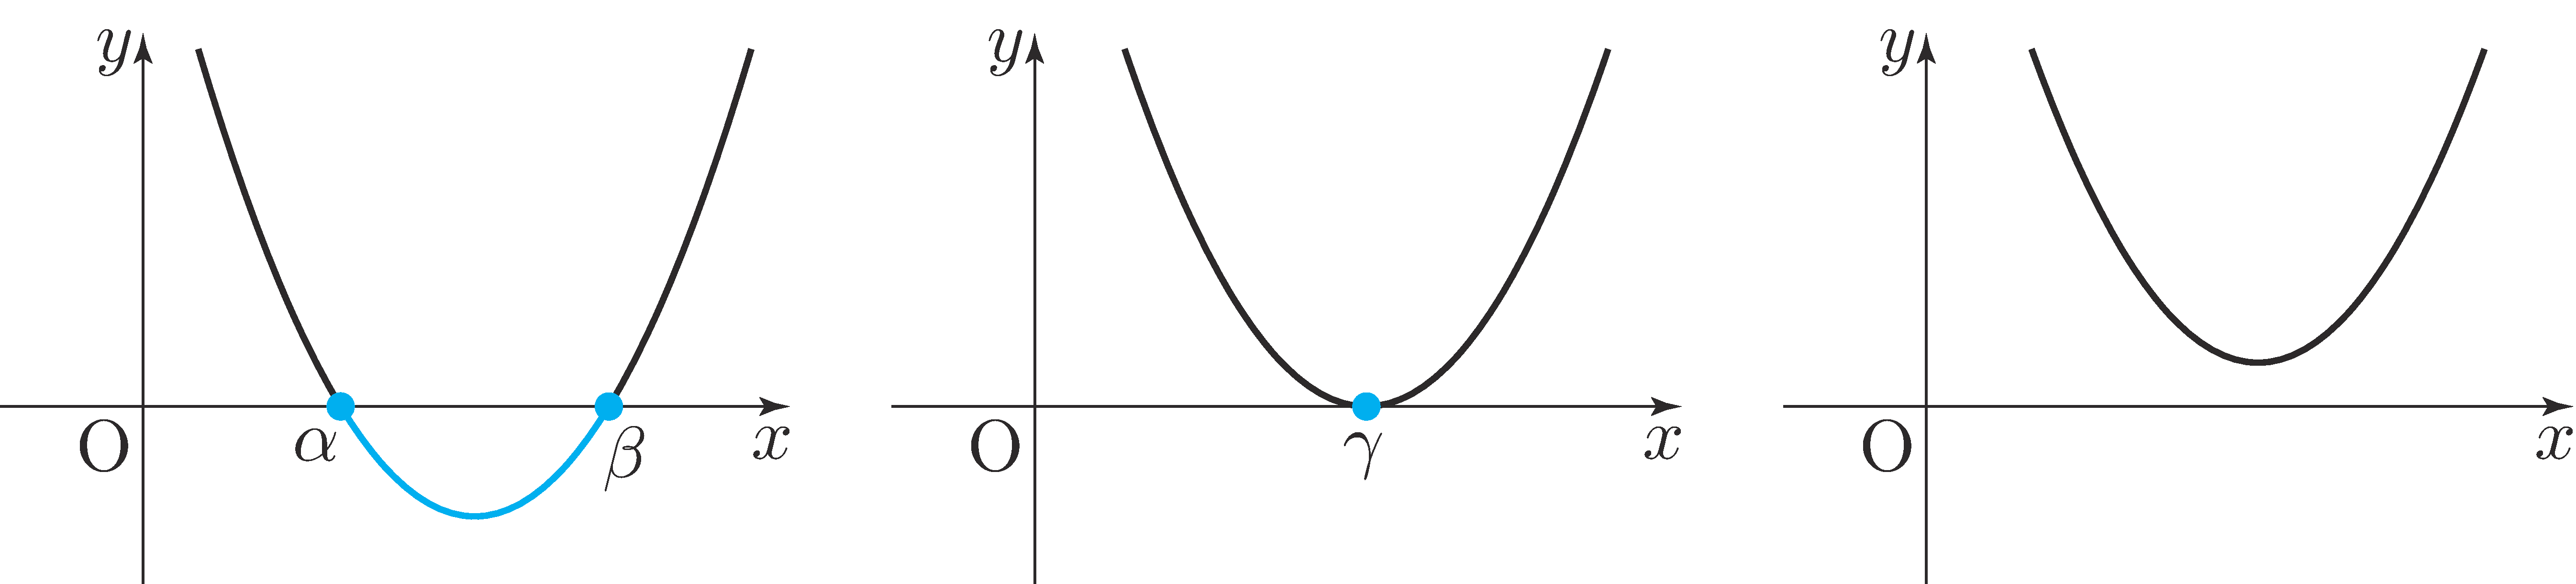
\includegraphics[scale=\pgfkeysvalueof{picsize}]{DBs/pic/zery_27.pdf}\
	\end{center}$a>0$일 때, $D>0$이면 $\CCI{\alpha}{\beta}$에 포함된 모든 실수가 부등식의 해입니다. $D=0$이면 $x=\gamma$가 부등식의 해입니다. $D<0$이면 부등식의 해가 없습니다.
\begin{center} 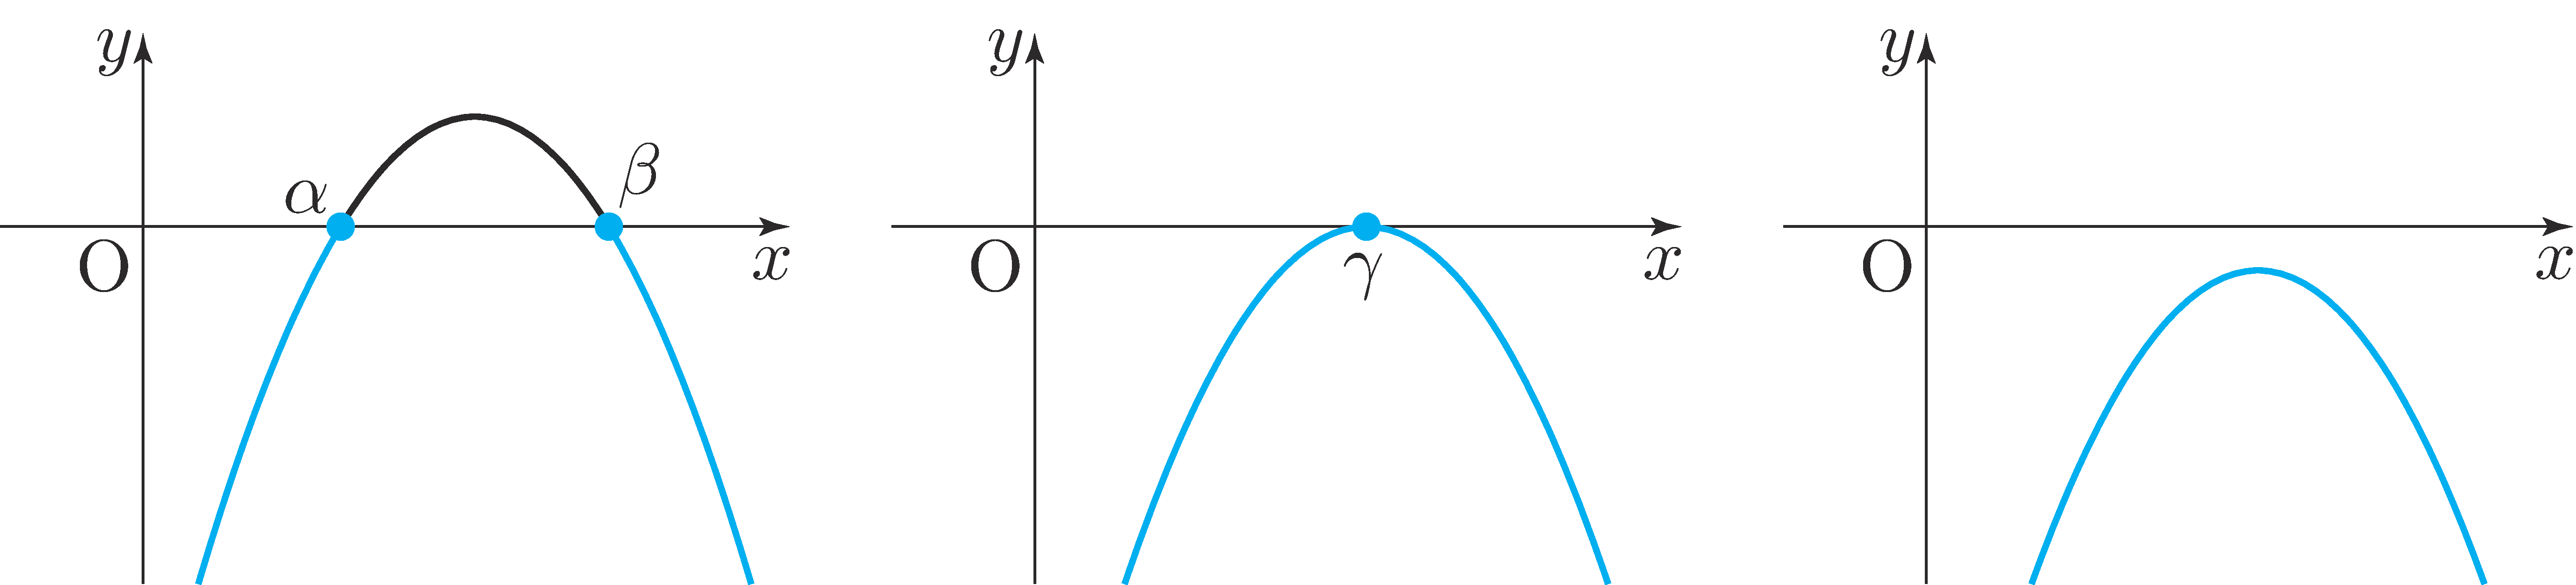
\includegraphics[scale=\pgfkeysvalueof{picsize}]{DBs/pic/zery_27_1.pdf}\
	\end{center}$a<0$일 때, $D>0$이면 $\OCI{-\infty}{\alpha}$, $\COI{\beta}{\infty}$에 포함된 모든 실수가 부등식의 해입니다. $D=0$이면 모든 실수가 부등식의 해입니다. $D<0$이면 모든 실수가 부등식의 해입니다.
\clearpage
\subsection{절대부등식과 이차부등식}
\subsubsection{절대부등식}
주어진 전체 범위에 포함된 임의의 실수에 대하여 성립하는 부등식을 \term{절대부등식}{}이라고 합니다. 절대부등식의 대표적인 예는 다음이 있습니다.\mn{절대부등식은 등호가 언제 성립하는지를 확인하는 것도 매우 중요합니다. 산술평균과 기하평균의 관계는 $a=b$일 때 등호가 성립합니다. 절댓값 부등식은 $a$와 $b$의 부호가 같을 때 또는 적어도 하나가 $0$일 때, 즉 $ab \ge 0$일 때 성립합니다.}{}
\begin{enumerate}[label={\onum*}]
	\item 산술평균과 기하평균의 관계 : 임의의 양수 $a$, $b$에 대하여 $\dfrac{a+b}{2} \ge \sqrt{ab}$
	\item 절댓값 부등식 : 임의의 실수 $a$, $b$에 대하여 $\abs{a} + \abs{b} \ge \abs{a+b} $
\end{enumerate}
\subsubsection{이차부등식이 절대부등식이 될 조건}
이차부등식이 임의의 실수 $x$에 대하여 성립한다면 이 또한 절대부등식입니다. 이차부등식이 절대부등식이 되기 위한 조건을 알아봅시다.
\begin{center} 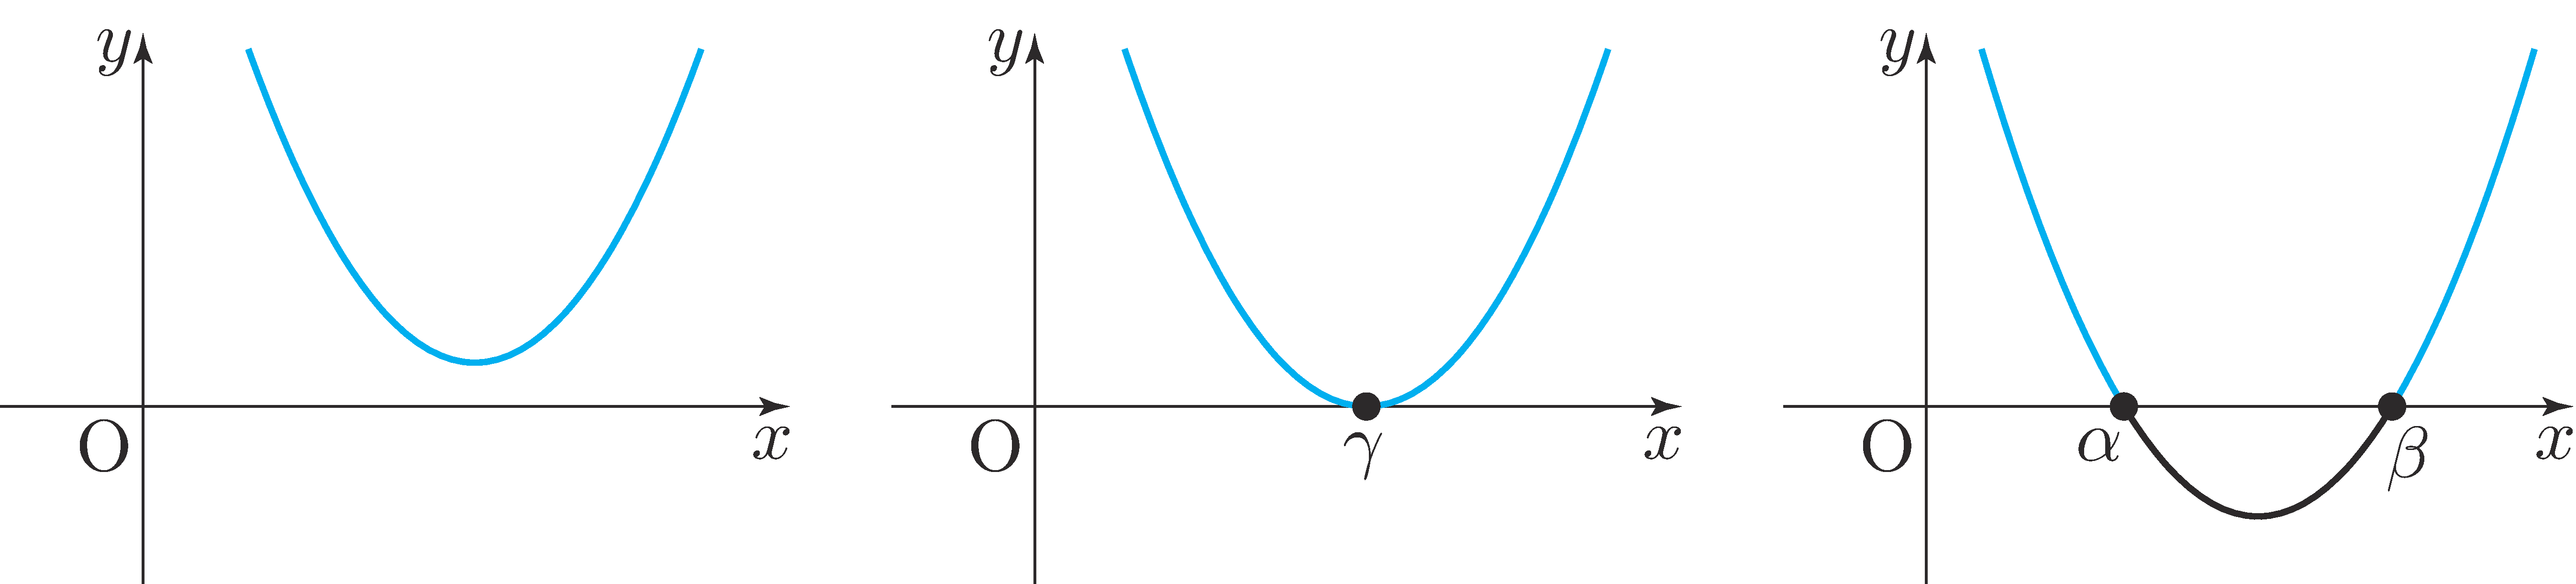
\includegraphics[scale=\pgfkeysvalueof{picsize}]{DBs/pic/zery_28.pdf}\
	\end{center}최고차항의 계수가 양수인 경우, $ax^2 + bx + c > 0$이 모든 실수 $x$에 대하여 성립하려면 $D<0$이어야 합니다. $D=0$이면 부등식이 성립하지 않도록 하는 실수 $\gamma$가 하나 존재하게 되고, $D>0$이면 $\CCI{\alpha}{\beta}$에 포함된 모든 실수 $x$가 부등식을 성립하지 않도록 하는 실수입니다.
\begin{center} 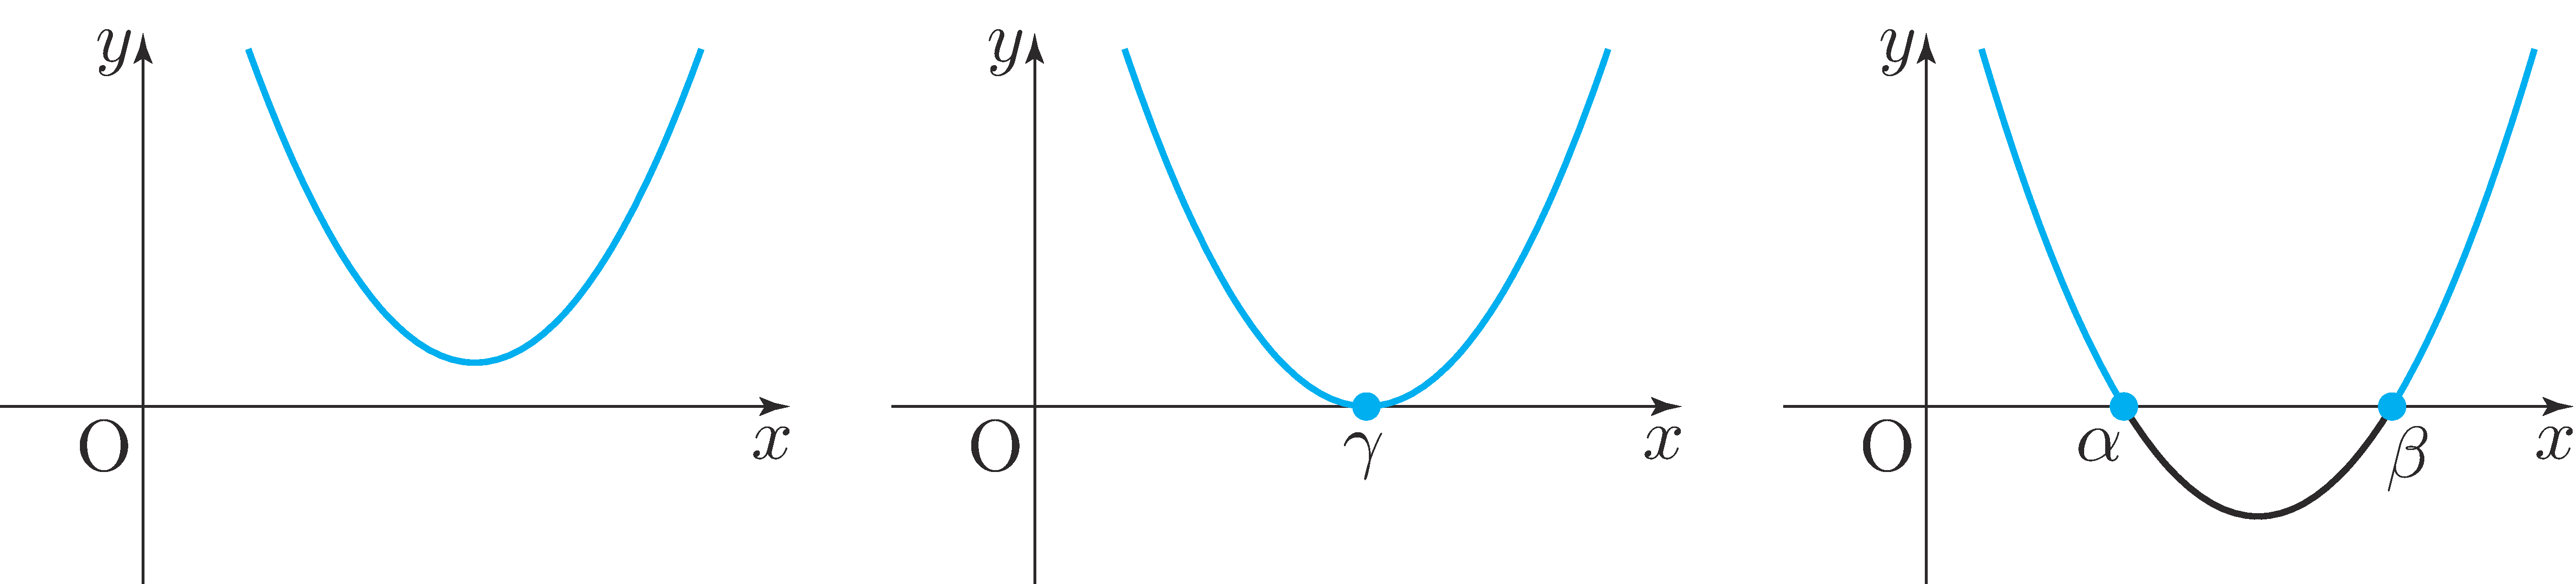
\includegraphics[scale=\pgfkeysvalueof{picsize}]{DBs/pic/zery_29.pdf}\
	\end{center}최고차항의 계수가 양수인 경우, $ax^2 + bx + c \ge 0$이 모든 실수 $x$에 대하여 성립하려면 $D \le 0$이어야 합니다. 이때 $D<0$이면 등호는 성립하지 않고, $D=0$이면 등호가 성립하도록 하는 실수가 하나 존재합니다. $D>0$이면 $\OOI{\alpha}{\beta}$에 포함된 모든 실수 $x$가 부등식을 성립하지 않도록 하는 실수입니다.
\clearpage\begin{center} 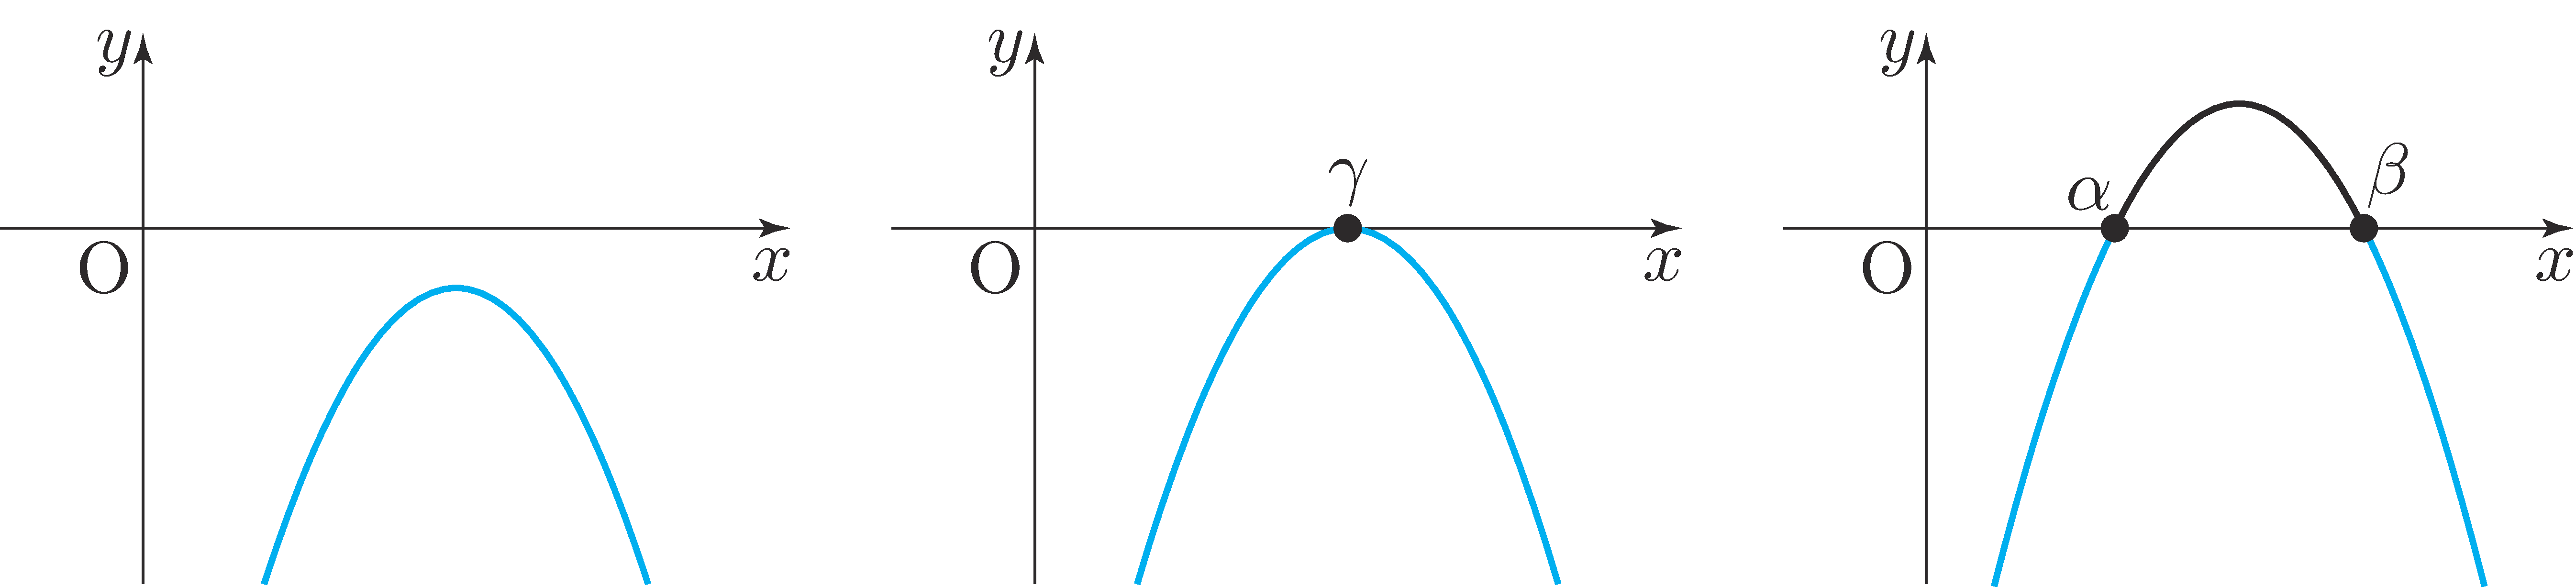
\includegraphics[scale=\pgfkeysvalueof{picsize}]{DBs/pic/zery_30.pdf}\
	\end{center}최고차항의 계수가 음수인 경우, $ax^2 + bx + c < 0$이 모든 실수 $x$에 대하여 성립하려면 $D<0$이어야 합니다. $D=0$이면 부등식이 성립하지 않도록 하는 실수 $\gamma$가 하나 존재하게 되고, $D>0$이면  $\CCI{\alpha}{\beta}$에 포함된 모든 실수 $x$가 부등식을 성립하지 않도록 하는 실수입니다.
\begin{center} 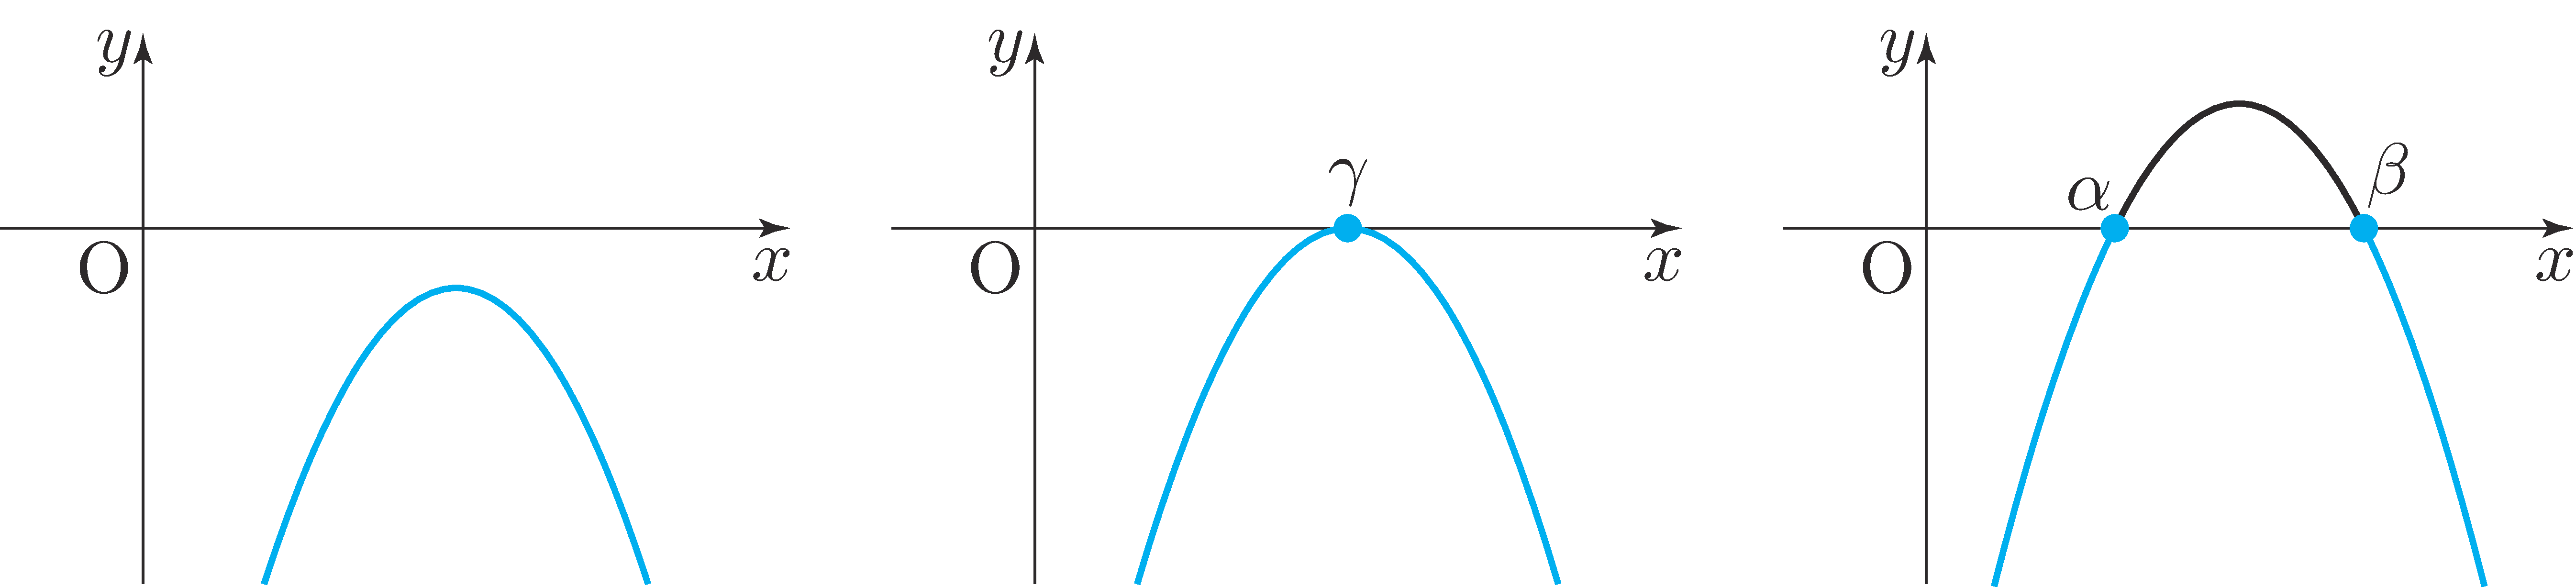
\includegraphics[scale=\pgfkeysvalueof{picsize}]{DBs/pic/zery_31.pdf}\
	\end{center}최고차항의 계수가 음수인 경우, $ax^2 + bx + c \le 0$이 모든 실수 $x$에 대하여 성립하려면 $D \le 0$이어야 합니다. 이때 $D<0$이면 등호는 성립하지 않고, $D=0$이면 등호가 성립하도록 하는 실수가 하나 존재합니다. $D>0$이면 $\OOI{\alpha}{\beta}$에 포함된 모든 실수 $x$가 부등식을 성립하지 않도록 하는 실수입니다.
